%% A minimalistic template for a PhD thesis. Complies with University of Liverpool's Code of Practice at the time of creation.
%% I would highly recommend to tinker with the template and make your thesis look the way you want it to look.
\documentclass[12pt,twoside]{report}
% \documentclass[lettersize,journal]{IEEEtran}

%% Use \includeonly to compile only some of the chapters. This will keep cross-references and page numbering intact as if all files have been compiled. For example (notice the relative paths!):
%\includeonly{./chapters/chapter1,./chapters/chapter3} 

%% Essential packages. Removing them might break the template.
% \usepackage[headheight=14pt,inner=3cm,outer=3cm]{geometry} % The minimal margins as specified by Code of Practice.
\usepackage[headheight=14pt,inner=3.8cm,outer=2.5cm]{geometry} % good for print

\usepackage{setspace}
\usepackage{datetime}
\usepackage{fancyhdr}
\usepackage{tikz}
\usepackage[caption=false, labelformat=parens, subrefformat=parens]{subfig}
\usepackage{makecell}
\usepackage{enumerate}
\usepackage{algpseudocode,amsmath}
\usepackage{booktabs}
\usepackage{setspace}
\usepackage{diagbox}
\usepackage{verbatim}
\usepackage{algorithm,algpseudocode}
\usepackage[acronym,nonumberlist,nopostdot]{glossaries}
\makenoidxglossaries
\usepackage{acronyms}
\usepackage{cite}
\usepackage{caption}
\usepackage{array, multirow}
\usepackage{tabularx} 
\usepackage[export]{adjustbox}
\usepackage[switch]{lineno}
\usepackage{longtable}
\usepackage{graphicx}
%% \BibTeX command to typeset BibTeX logo in the docs
\AtBeginDocument{%
  \providecommand\BibTeX{{%
    Bib\TeX}}}

%% Insert your packages here:
\usepackage{amssymb,amsmath,amsthm}
%\usepackage{microtype} % Makes the text look "nicer". Try with and without and choose for yourself.
\usepackage[hidelinks]{hyperref} % It is often advices to load hyperref last (there are exceptions).
%%

%% Insert your commands here:
\setcounter{tocdepth}{1}
\newcolumntype{?}{!{\vrule width 1pt}}
\captionsetup[table]{skip=5pt}
\newcommand{\multiline}[2]{%
  \begin{tabularx}{#1\textwidth}[t]{@{}X@{}}
    #2
  \end{tabularx}}
%%

\onehalfspacing % As adviced by Code of Practice. 

\graphicspath{{./figures/}{../figures/}} % Location of the figures and graphics files so that you can insert them without specifying a path to the figures folder.
\makeatletter
%% Insert your title and name.
\title{Robust Cardiac Feature Monitoring based on Millimeter-Wave Radar} \let\Title\@title
\author{Yuanyuan Zhang} \let\Author\@author
\makeatother

\begin{document}
%% The title page uses the title and author name specified above. No need to edit title.tex. Note that the current month is at the bottom of the title page. Edit it manually, if you want to have some other month there.
\pagestyle{empty}
\include{title}
\cleardoublepage

\begin{singlespace}
\pagenumbering{roman}
\onehalfspacing
\doublespacing

\addcontentsline{toc}{chapter}{Abstract} % Add the abstract to the table of contents.
\chapter*{Abstract}
% \thispagestyle{fancy}

Paraphrasing the Code of Practice: each copy of the thesis must contain an abstract indicating the aims of the investigation and  the  results  achieved.  It  should  be  no  longer  than  one  side  of  an  A4  sheet (normally  about 450  words).
\cleardoublepage

\addcontentsline{toc}{chapter}{Acknowledgements} % Add the acknowledgements to the table of contents.
\chapter*{Acknowledgements}
Travel back to 2022, I can still feel the confusion and 
\cleardoublepage

\addcontentsline{toc}{chapter}{Publications} % Add the publication list to the table of contents.
\chapter*{Publications}
\section*{Journal paper:}
% `` and ''
\begin{enumerate}
	\item \textbf{Yuanyuan Zhang}, Runwei Guan, Lingxiao Li, Rui Yang, Yutao Yue, Eng Gee Lim, `` radarODE: An ODE-Embedded Deep Learning Model for Contactless ECG Reconstruction from Millimeter-Wave Radar'', \textit{\textbf{IEEE Transactions on Mobile Computing},} Apr. 2025.
	\item \textbf{Yuanyuan Zhang}, Rui Yang, Yutao Yue, Eng Gee Lim, ``radarODE-MTL: A Multi-Task Learning Framework with Eccentric Gradient Alignment for Robust Radar-Based ECG Reconstruction'', \textit{\textbf{IEEE Transactions on Instrumentation and Measurement},} Apr. 2025.
    \item \textbf{Yuanyuan Zhang}, Rui Yang, Yutao Yue, Eng Gee Lim, Zidong Wang, ``An Overview of Algorithms for Contactless Cardiac Feature Extraction From Radar Signals: Advances and Challenges'', \textit{\textbf{IEEE Transactions on Instrumentation and Measurement}}, Jul. 2023.
    % \item Runwei Guan, KaLok Man, Liye Jia, \textbf{Yuanyuan Zhang}, Shanliang Yao, EngGee Lim, Jeremy Smith, Yutao Yue, "Traffic Accident Scene Recognition with FMCW Radar and Vision Transformer", \textit{\textbf{International Journal of Design, Analysis and Tools for Integrated Circuits and Systems}}, Nov. 2022.
\end{enumerate}

\section*{Conference paper:}
\begin{enumerate}
	\item \textbf{Yuanyuan Zhang}, Sijie Xiong, Rui Yang, Eng Gee Lim, Yutao Yue, ``Recover from Horcrux: A Spectrogram Augmentation Method for Cardiac Feature Monitoring from Radar Signal Components'', \textit{in 2025 47th Annual International Conference of the IEEE Engineering in Medicine \& Biology Society (\textbf{EMBC2025}),} IEEE, Jul. 2025. 
\end{enumerate}

\section*{Under Review:}
\begin{enumerate}
    \item \textbf{Yuanyuan Zhang}, Haocheng Zhao, Sijie Xiong, Rui Yang, Eng Gee Lim, Yutao Yue, ``From High-SNR Radar Signal to ECG: A Transfer Learning Model with Cardio-Focusing Algorithm for Scenarios with Limited Data'', \textit{\textbf{IEEE Transactions on Mobile Computing}}. (Under Review)
    \item Sijie Xiong, \textbf{Yuanyuan Zhang}, Cheng Tang, Haoling Xiong, Yiding Li, Atsushi Shimada, ``U-MA: A Unified Framework with Differential Mamba under Parallel U-Net Scheme for Time Series Forecasting'', \textit{\textbf{Engineering Applications of Artificial Intelligence}}. (Under Review)
    \item Sijie Xiong, Cheng Tang, \textbf{Yuanyuan Zhang}, Haoling Xiong, Youhao Xu, Atsushi Shimada, ``CME-Mamba with Enhancing Nonlinear Dependencies for Time Series Forecasting'', \textit{\textbf{Applied Soft Computing}}. (Under Review)
\end{enumerate}


\cleardoublepage

\tableofcontents
\addcontentsline{toc}{chapter}{Contents} % Add the the table of contents to the table of contents.
\clearpage

\listoffigures
\addcontentsline{toc}{chapter}{List of Figures} % Add the list of figures to the table of contents.
\clearpage

\listoftables
\addcontentsline{toc}{chapter}{List of Tables} % Add the list of tables to the table of contents.
\clearpage

\addcontentsline{toc}{chapter}{List of Acronyms} % Add the list of tables to the table of contents.
\glsnogroupskiptrue
\setglossarystyle{super}
\renewcommand{\glsnamefont}[1]{\textbf{#1}}
% \glsaddall
\printnoidxglossaries

\clearpage

%% You might need a similar construction to include the list of algorithms.

\end{singlespace}
\cleardoublepage

%% In the thesis, pages are numbered with arabic numerals in the top outer corners (left top corner on even numbered pages, and right top corner on odd numbered pages) and alternatively Author and Chapter: Chapter name in the other top corner.
\pagenumbering{arabic}
\pagestyle{fancy}
\fancyhead{} % clear all header fields
\fancyhead[LE,RO]{\bfseries\thepage}    % Page number (boldface) in left on even
% pages and right on odd pages
\renewcommand{\chaptermark}[1]{\markboth{\chaptername\ \thechapter.\ #1}{}}
\fancyhead[RE]{\bfseries\nouppercase{\leftmark}}      % Chapter in the right on even pages
\fancyhead[LO]{\bfseries\nouppercase{\rightmark}}     % Section in the left on odd pages

\fancyfoot{} % clear all footer fields

\chapter{Introduction} % Write in your own chapter title
\label{ch:intro} % Add a label in case you want to refer to the chapter.

\glsresetall
\chapter{Background and Literature Review} \label{ch:LR}
In this chapter, the necessary background for radar theory and radar-based vital sign monitoring is first provided for a better understanding of the proposed methods in the later chapters. In addition, representative signal processing and deep learning methods for cardiac feature extraction are also introduced to provide a comprehensive review of the development over the last decade.

\section{Background Knowledge}
\subsection{Radar Types}
Different radar systems transmit different types of waveforms as shown in Figure~\ref{fig:intro_overall}(b). For example, \gls{cw} radar uses continuous wave with a fixed frequency, FMCW radar uses continuous wave with linearly increased frequency, and \gls{uwb} radar uses pulses with wide frequency bandwidth. The phase components of the transmitted signals for CW and FMCW radar are modulated by the displacement composed by respiration, heartbeat and all kinds of noises in a non-linear manner as proved in~\cite{chen2021movi,li2013review}. Then, the phase variation hidden in the raw received signal can be revealed using phase unwrapping techniques such as arctangent demodulation and extended differentiate and cross-multiply algorithm~\cite{obadi2021survey,wang2020remote}. For IR-UWB radar, the cardiac features are embedded in the propagation time delay of the echo signal~\cite{obadi2021survey}. 

Different radar types require different architectures and are suitable for different tasks. For example, CW radar has a simple architecture and adopts the fundamental baseband signal-processing methods, but the range information cannot be extracted from the received signals due to the lack of modulation~\cite{singh2020multi}. FMCW radar outperforms CW radar by leveraging the frequency modulation techniques, improving the \gls{snr} and providing the capability of range detection to further isolate the signal reflected only from the chest region~\cite{ha2020contactless}. Different from the continuous waveform used in CW and FMCW radar, IR-UWB radar emits widely spaced pulses with very short duration (e.g., $0.1-2$ ns)~\cite{hirt2003ultra}. Therefore, IR-UWB radar is more power-efficient than FMCW radar but normally cannot ensure a high SNR and range resolution~\cite{obadi2021survey}. In literature, IR-UWB radar is normally used for through-the-wall or long-distance monitoring~\cite{shen2018respiration}, but the complex radar architecture (e.g., requiring internal delay calibration~\cite{singh2020multi}) and signal-processing algorithms (e.g., harmonic rejection~\cite{wang2020experimental}) limit the relative research\cite{li2013review}.
        
In addition to the different radar types, radar operating frequency (carrier frequency) is another crucial parameter affecting cardiac monitoring quality because the frequency is inversely related to the beamwidth for antennas with the same diameter~\cite{huang2021antennas}, enabling the radar system with high operating frequency using narrow beamwidth to enhance directivity~\cite{ramasubramanian2018moving}.  Obeid \textit{et al.}~\cite{obeid2008low} found out that high operating frequency provides a large phase difference caused by heart vibration and improves the sensitivity of cardiac monitoring. The researchers in~\cite{ramasubramanian2018moving} claimed that the radar with a high operating frequency, especially the mmWave range ($30-300$ GHz), can achieve a high range resolution, good noise-robustness and small antenna size.

According to the review of the trends in radar usage for the recent decade, CW radar was the most popular type before 2020 due to its simple architecture; FMCW radar receives a growing concern since 2015 because the recent-released commercial FMCW radar platforms reduce the knowledge required for designing or setting up a radar system~\cite{zhou2022towards}; IR-UWB radar is less popular than the other two types due to its complex radar architecture and signal-processing algorithms~\cite{singh2020multi,wang2020experimental}. For the trend in operating frequency selection, early studies all focus on the low-frequency band for the simplicity of radar architecture design and baseband signal-processing algorithms, whereas the recent researchers are steering toward using mmWave radar (especially $60$ or $77$ GHz commercial radar platform) for good performance. In summary, the FMCW with high operating frequency is becoming the mainstream for radar-based cardiac monitoring due to the balance between the performance and complexity, and the complexity for settling the radar platform is also significantly reduced due to the emergency of commercial radar.

\subsection{Theoretical Background for Vital Sign Monitoring}
\subsubsection{Cardiac Signal Extraction from CW Radar}
The vanilla signal model for radar-based cardiac monitoring (e.g., heart rate monitoring) using CW radar starts from the transmitted signal expressed as
\begin{equation}
s_t(t)=A_t\cdot\cos (2 \pi f t+\theta(t))
\end{equation}
where $A_t$ and $f$ are the amplitude and carrier frequency of the transmitted signal, and $\theta(t)$ is the phase noise from the signal generator with respect to time $t$~\cite{droitcour2004range}. In the ideal case, the radar signal is only reflected by a human at a fixed distance $d_0$ with a varying chest displacement as $x(t)$, and the received signal after propagation time $T_p(t)$ can be derived as
\begin{equation}
s_r(t)=A_r\cdot\cos (2 \pi f (t-T_p(t))+\theta(t-T_p(t)))
\end{equation}
with
\begin{equation}
\begin{aligned}
T_p(t) &= \frac{2d(t)}{c} \\
d(t) &= d_0+x(t)
 \end{aligned}
\end{equation}
where $A_r$ is the amplitude of the received signal, $c$ is the light speed and $2d(t)$ represents the round trip distance of the signal between the transmitter and receiver. Then, the received signal can be expanded as
\begin{equation}
s_r(t)=A_r\cdot\cos (2 \pi ft-\frac{4\pi d_0}{\lambda}-\frac{4\pi x(t)}{\lambda}+\theta(t-\frac{2 d_0}{c}-\frac{2 x(t)}{c}))
\end{equation}
where $\lambda$ is the wavelength that equals to $\frac{c}{f}$. According to~\cite{droitcour2004range,lin2022broadband}, it is safe to eliminate changes in amplitude and phase noise term because the chest displacement is much less than the fixed distance (i.e., $x(t)\ll d_0$). Therefore, the approximate received signal is
\begin{equation}
s_r(t)\approx \cos (2 \pi ft-\frac{4\pi d_0}{\lambda}-\frac{4\pi x(t)}{\lambda}+\theta(t-\frac{2 d_0}{c}))
\end{equation}

The received signal $s_r(t)$ will then pass a local oscillator with a low-pass filter to remove the frequency term, and the resultant baseband signal is
\begin{equation}
s_b(t)=cos(\theta_d+\frac{4\pi x(t)}{\lambda}+\Delta \theta(t))
\end{equation}
with
\begin{equation}
\begin{aligned}
 \theta_d &= \frac{4\pi d_0}{\lambda} + \theta_{0}\\
\Delta \theta (t) &= \theta(t)- \theta(t-\frac{2 d_0}{c})
 \end{aligned}
\end{equation}
where $\theta_d$, $\theta_0$ and $\Delta \theta (t)$ are phase shifts affected by different factors such as $d_0$, signal mixer and antenna, and can be set as constant~\cite{lin2022broadband}. Then, the phase signal unwrapped from the baseband signal is obtained as
\begin{equation}
\phi(t) = \theta_d+\frac{4\pi x(t)}{\lambda}+\Delta \theta(t)
\end{equation}

Finally, the vanilla signal model derived above shows that the chest displacement $x(t)$ is involved in the phase variation of the baseband signal as
\begin{equation}\label{equ:phase1}
\Delta\phi(t) = \frac{4\pi x(t)}{\lambda}
\end{equation}

The follow-up researchers have proposed various techniques to improve the accuracy of the unwrapped phase signal variation in (\ref{equ:phase1}). For example, the in-phase/quadrature modulation is proposed to solve the null point issue~\cite{droitcour2004range}; the differentiate and cross-multiply algorithm is designed to avoid discontinuity in the unwrapped phase signal~\cite{zhang2023overview}. In addition, chest displacement $x(t)$ is a mixture of cardiac activities, respiration and noises (e.g., \gls{rbm}~\cite{chen2021movi,zhang2020health}, multi-path or multi-person interference~\cite{mercuri2021enabling,islam2022contactless}). Therefore, enormous advanced algorithms are proposed to decompose cardiac information from $x(t)$, as have been reviewed in~\cite{zhang2023overview}.

\subsubsection{Cardiac Signal Extraction from FMCW Radar}
FMCW could provide advanced features that allows the extraction of the signal reflected from certain points. In the literature, FMCW radar has been widely used in nowadays \gls{mmWave} sensing to measure the range, velocity and \gls{aoa} of the objects appearing in the field of view~\cite{tang2024bsense}, with three critical concepts that configure the transmitted waveform:
\begin{itemize}
\item \textbf{Chirp } is the minimum component in the FMCW signal with microsecond-level duration and is often called fast time. The waveform of a single chirp is a sinusoidal signal with frequency that changes linearly over time, with the key characteristics designated by start frequency, bandwidth and chirp duration to get range information of the object.
\item \textbf{Frame} is a collection of multiple chirps that forms a complete observation window to get the velocity information based on the range bins extracted from chirps and is often referred to as slow time.
\item \textbf{Virtual antenna array (channel)} is a commonly used concept in \gls{mimo} radar systems and is able to realize complex modulations or beamforming~\cite{xiong2022vital}. However, this study mainly leverages the phase difference across antenna channels to estimate the AoA of the objects.
\end{itemize}
The popular commercial radar platforms have provided a convenient interface for radar configuration, signal modulation and demodulation~\cite{AWR1843}, and the reflected signal from a give point $E=(x,y,z)$ in 3D space can be expressed as:
\begin{equation}\label{equ:raw_sig}
R(E, t)=\sum_{v=1}^V \sum_{c=1}^C \sum_{n=1}^N s_{v, c, n}(t)\cdot e^{j 2 \pi \frac{2k\cdot d(E, v)}{\text{light speed}} n} \underbrace{e^{j 2 \pi \frac{2\cdot d(E, v)}{\lambda}}}_{\text{phase term}\ \phi}
\end{equation}
where $(x,y,z)$ represents the (horizontal, radial, vertical) axis, $V$ is the number of virtual antenna channels, $C$ means the number of chirps within one frame, $N$ is the total sample points within one chirp, $s_{v, c, n}(t)$ denotes the original received signal, $k$ is the slope of frequency raising, $\lambda$ means wavelength and $d(E, v)$ represents the distance between point $E$ and virtual antenna $v$~\cite{chen2022contactless}. In FMCW processing for vital sign monitoring, the time sample $t$ corresponds to one frame instead of the sample point $n$, and the signal from different chirps $c$ and antenna channels $v$ will be accumulated to improve SNR~\cite{liu2024diversity}.

The interested term in (\ref{equ:raw_sig}) is the variation of distance $d(E,v)$, because it represents the displacements caused by respiration and heartbeat (without considering any other noise). Therefore, the chest region displacement $h(E, t)$ can be unwrapped from phase variation $\Delta \phi$ as
\begin{equation}\label{equ:phase}
h(E, t) = \frac{\lambda \Delta \phi}{4\pi}
\end{equation}

At last, some common noises, such as respiration and thermal noise, can be easily removed using a band-pass filter and differentiator to make sure that the final $h(E, t)$ mostly contains cardiac-related features from point $E$. 

\subsection{Radar-Based ECG Monitoring as a Domain Transformation Problem}
Coarse cardiac monitoring only aims to detect a single heartbeat within one cardiac cycle, while fine-grained cardiac monitoring requires recovering subtle cardiac activities within one cardiac cycle. For example, Figure~\ref{fig:scg_ecg} shows the typical radar and SCG signal waveform within a single cardiac cycle that describes the cardiac mechanical activities, such as aortic valve opening/closure (AO/AC) and mitral valve opening/closure (MO/MC)~\cite{swift2021stop,orkand1964heart}. These mechanical activities are muscle contractions stimulated by cardiac electrical events, such as P-wave, QRS-complex and P-wave in the ECG signal as shown in Figure~\ref{fig:scg_ecg}. Therefore, radar-based ECG recovery is actually a domain transformation problem that translates cardiac mechanical activities into electrical activities and realizes fine-grained vital sign monitoring in a contactless manner.
 \begin{figure}[tb] 
    \centering 
    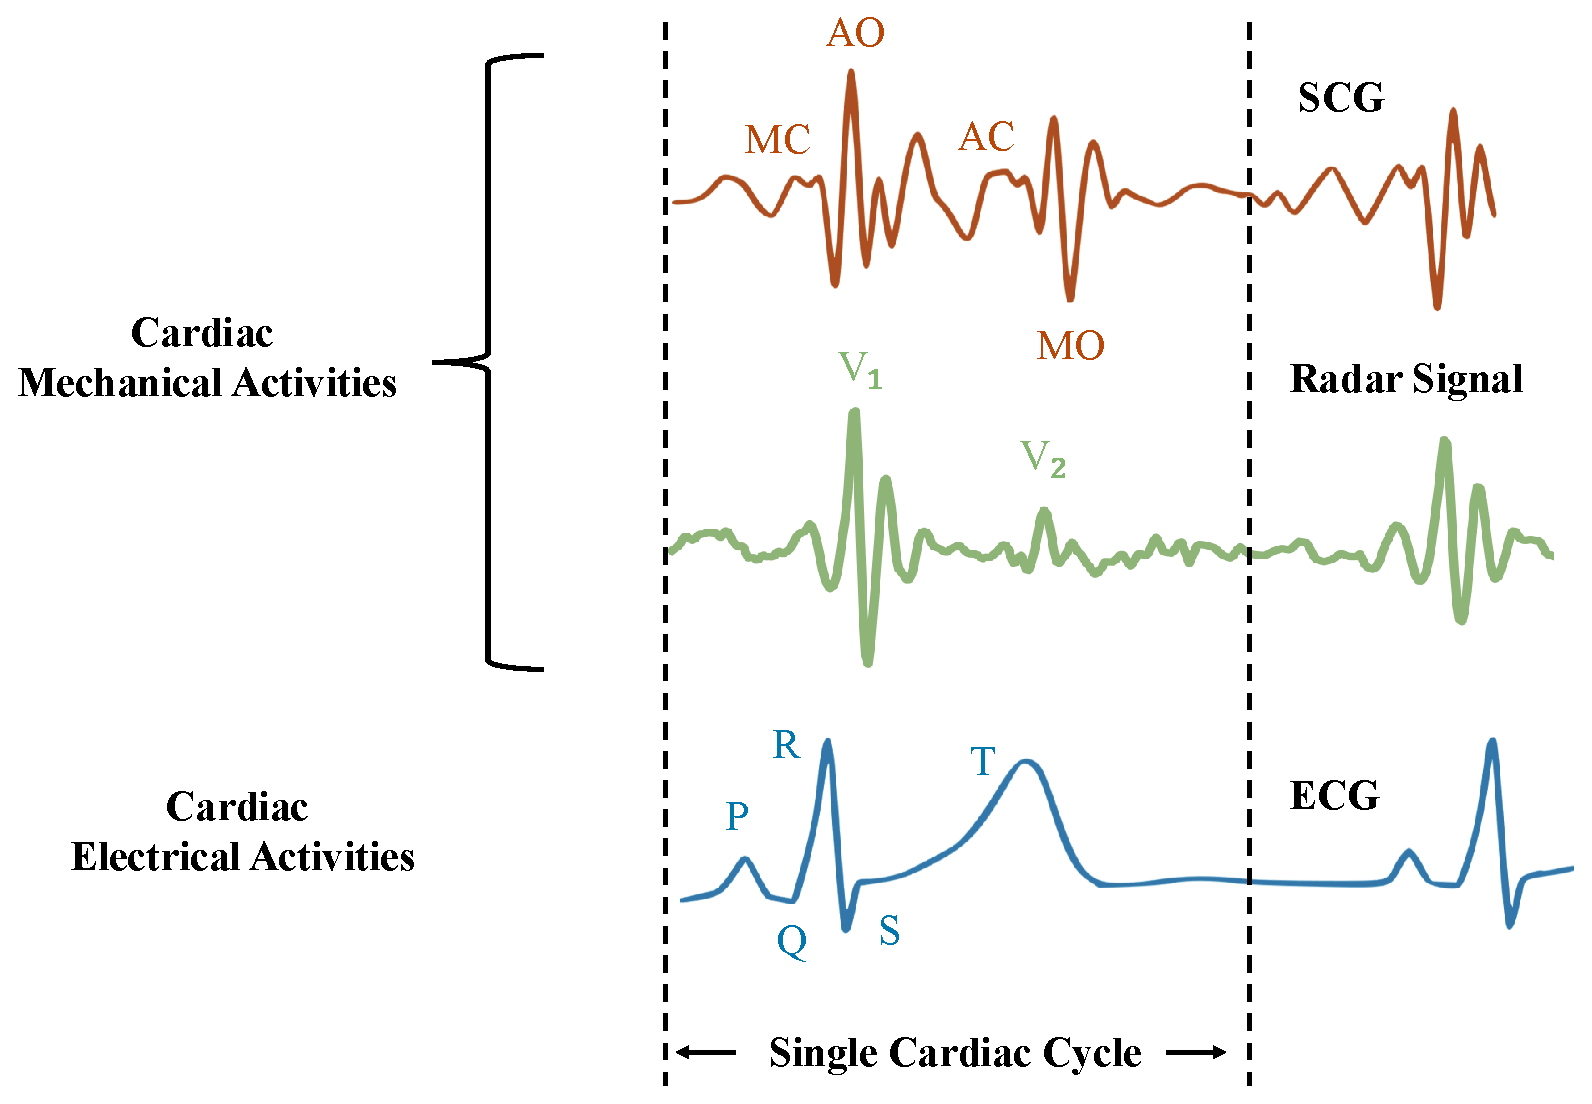
\includegraphics[width=0.8\columnwidth]{scg_ecg.eps}
    \caption{Relationships between cardiac mechanical and electrical activities within the same cardiac cycle.} 
    \label{fig:scg_ecg} 
\end{figure}
In the literature, the domain transformation is only realized by deep-learning-based methods, while a common issue of the deep learning model is not robust against large-scale noise (e.g., RBM) as reported by many previous studies~\cite{wu2023contactless,li2024radarnet,wang2023ecg,zhao2024airecg}. However, there is no existing work that investigates the noise-robustness of the deep learning model itself, and this thesis is motivated to develop a noise-robust deep learning model to realize the domain transformation in the presence of body movement noise.

\section{Literature Review for Cardiac Feature Extraction}
\subsection{Spectrum-based Methods}
Spectrum represents the transformation of signal from time-domain to frequency-domain and can reveal the main frequency components of the signal~\cite{petrovic2019high, saluja2019supervised, yang2020vital, zhu2018fundamental, le2020heartbeat, zhao2016emotion, xiong2020differential, hu2014real, xiong2017accurate, tu2015fast, park2017polyphase, shih2021quadrature, tomii2015heartbeat, li2017wavelet, mercuri2019vital, wang2020remote, liu2022vital, ling2022non}. Normally, the \gls{rr}) and HR frequency at rest are in the range of $0.1-0.5$ Hz and $1-1.6$ Hz respectively~\cite{mogi2017heartbeat}, making the spectrum-based method the most straightforward way to extract cardiac features within a certain frequency range. The spectrum-based methods usually share similar ideas: (a) a piece of unwrapped phase signal taken from the dataset only shows the periodic displacement induced by strong respiration instead of subtle cardiac activities as shown in Figure~\ref{fig:rawRadar}; (b) the raw signal is then transformed into a spectrum using time-frequency transformation methods (e.g., \gls{fft}, \gls{cwt}) as shown in Figure~\ref{fig:rawRadar_fft} with corresponding peaks labelled; (c) for the low-noise scenario, after filtering the frequency components of RR, RR harmonic and other high-frequency noise, the remaining dominant peak of the spectrum represents the HR frequency; (d) for the noisy scenario, the researchers could use several techniques, such as noise-cancellation filter or differentiator, to suppress the noise or enhance the HR frequency component on the spectrum.

\begin{figure}[tbp]
    \centering
    \subfloat[]{\label{fig:rawRadar}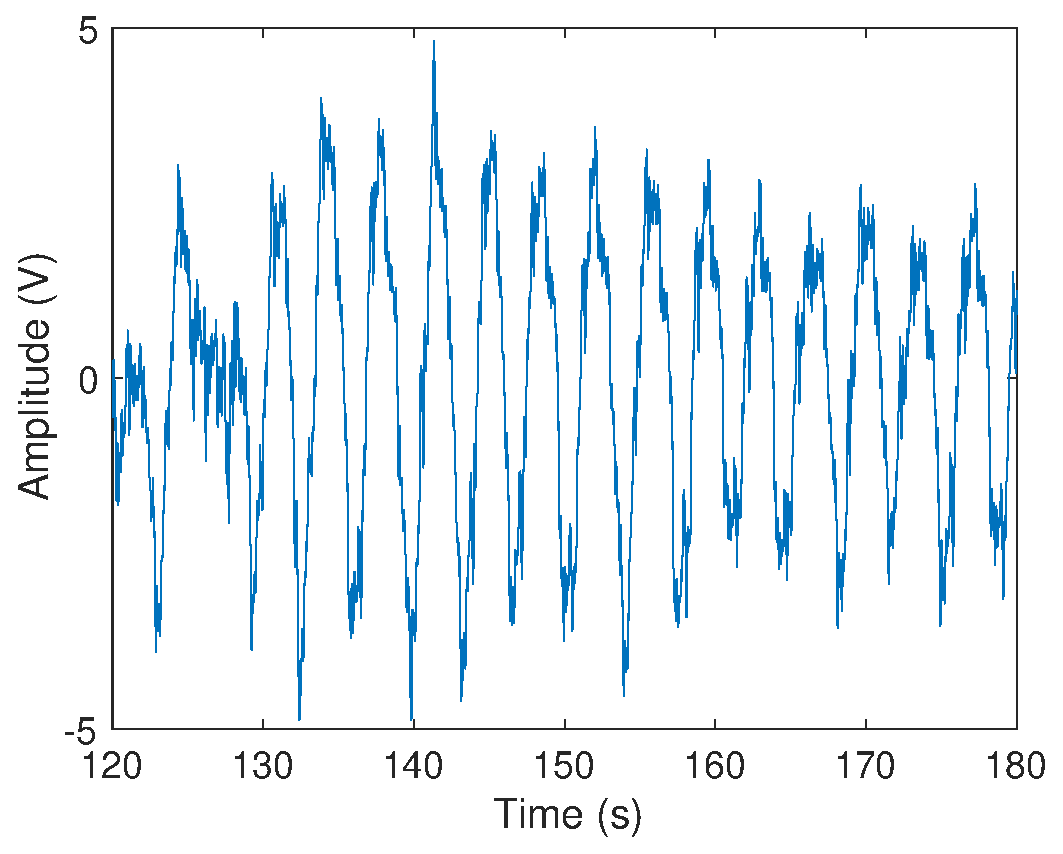
\includegraphics[width=0.25\columnwidth]{raw.eps}}
    \subfloat[]{\label{fig:rawRadar_fft}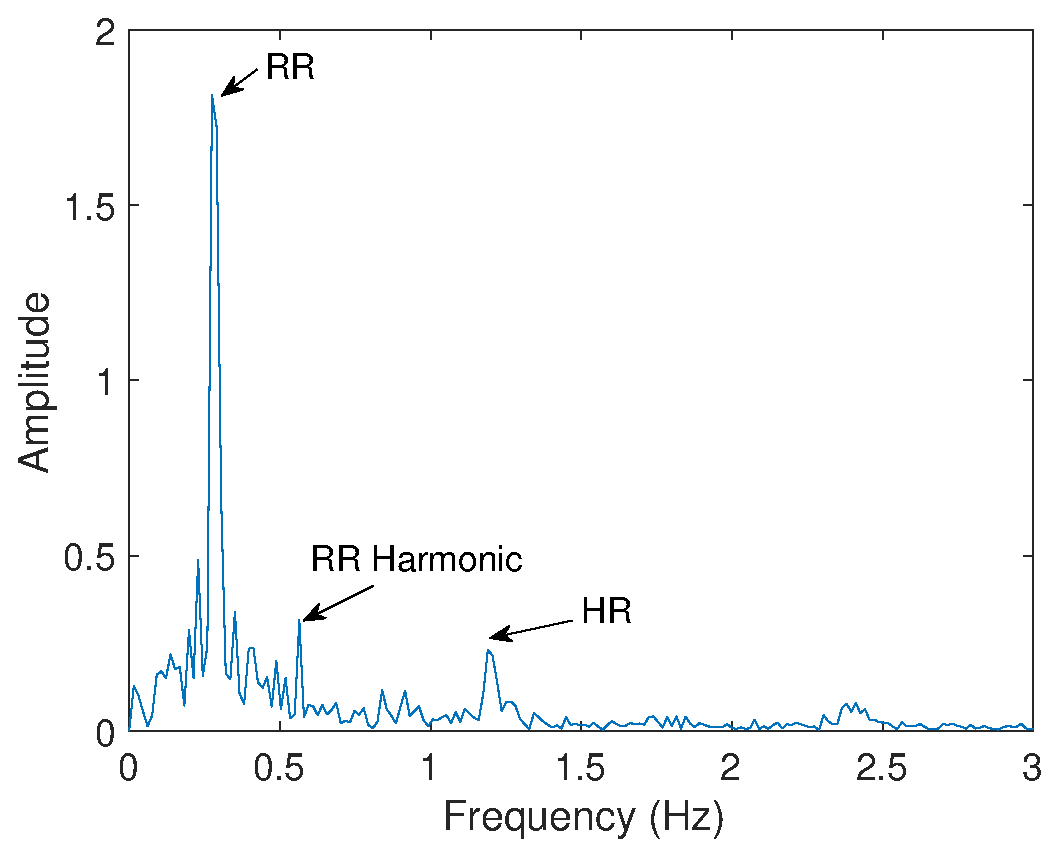
\includegraphics[width=0.25\columnwidth]{fft.eps}} 
    \subfloat[]{\label{fig:rawRadar_diff}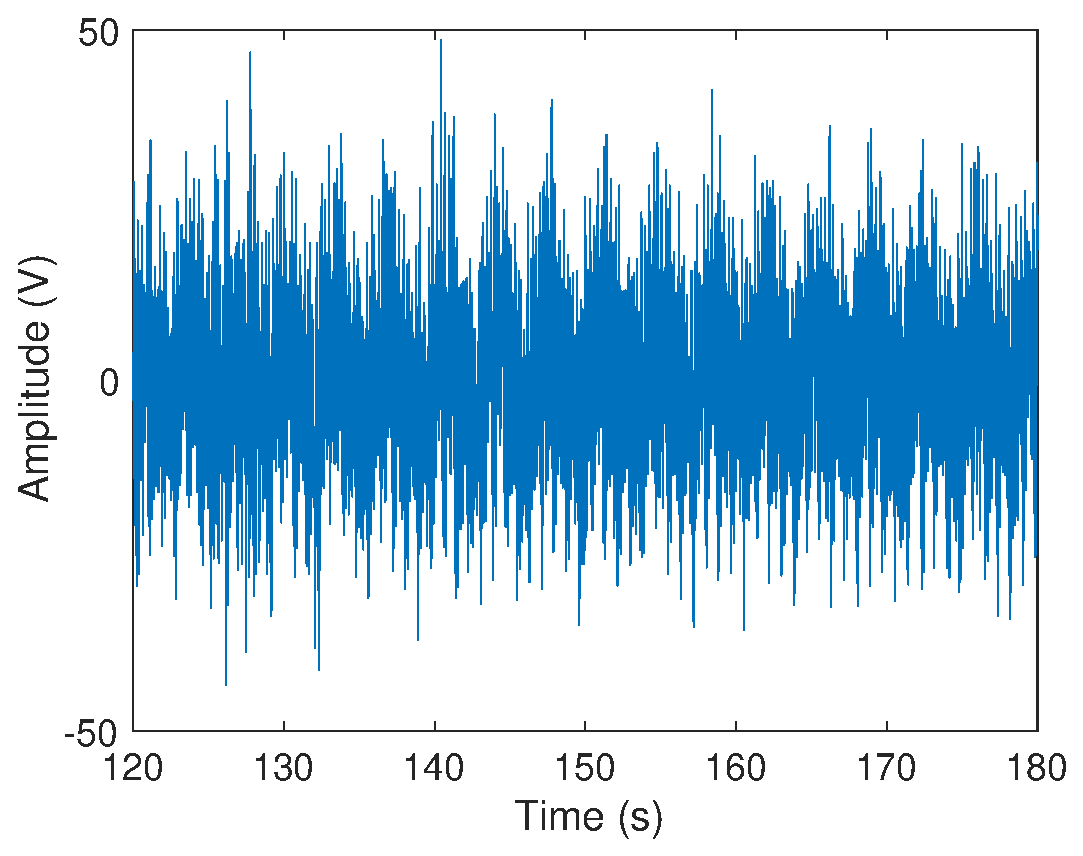
\includegraphics[width=0.25\columnwidth]{rawRadar_diff.eps}}
    \subfloat[]{\label{fig:rawRadar_diff_fft}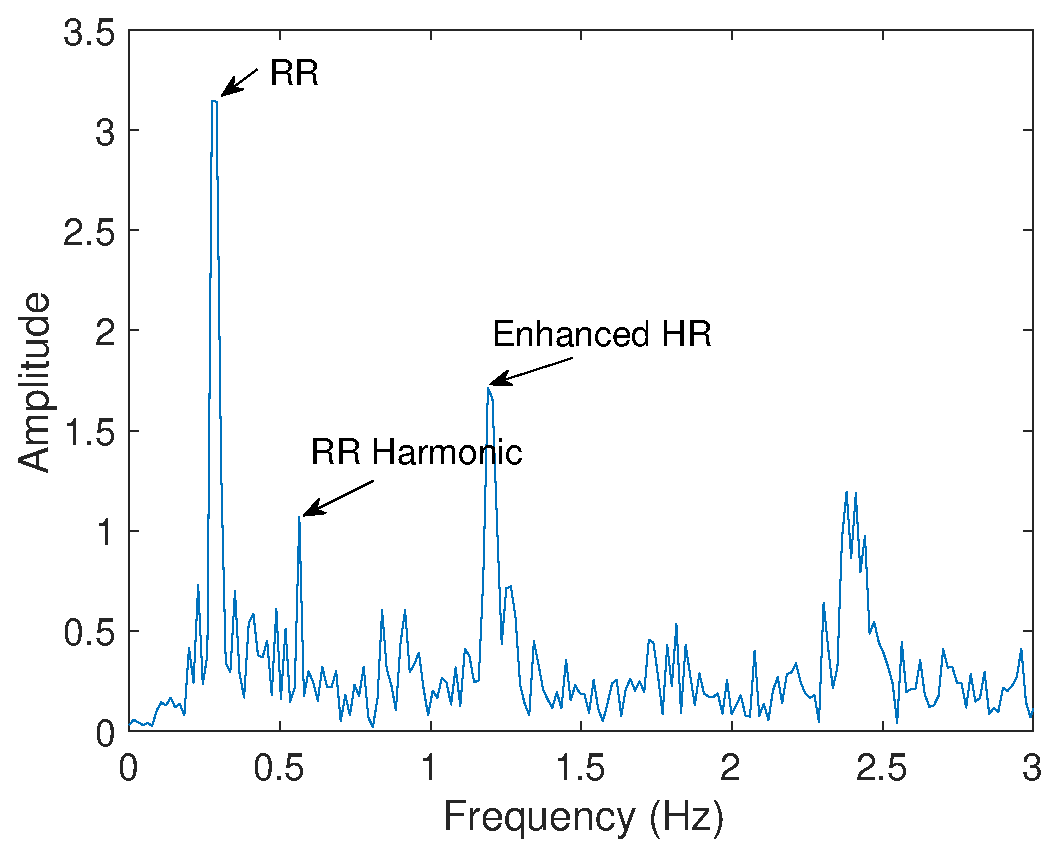
\includegraphics[width=0.25\columnwidth]{fftForHR_diff.eps}} 
    \caption{Illustration for spectrum-based methods: (a) raw radar signal; (b) spectrum obtained for raw radar signal from FFT, with RR, RR harmonic and HR peaks labelled; (c) raw radar signal after differentiation; (d) spectrum obtained for differentiated raw radar signal from FFT, with enhanced HR peak labelled.}
    \label{fig:fftForHR}
\end{figure}

\subsubsection*{Evaluations}
The spectrum-based methods are matured in the signal-processing area and can be implemented directly on the hardware with limited computational resources while achieving good real-time performance~\cite{hu2014real,park2017polyphase}. In fact, several commercial data-capture boards for raw radar signal processing have already embedded these algorithms on \gls{fpga}~\cite{obadi2021survey}. For the disadvantages, the spectrum-based methods are not sensitive to the abrupt HRV, because multiple cardiac cycles are involved in a single segment truncated by the time window, but only one HR value can be estimated from each segment~\cite{shi2021contactless}. Another problem caused by the truncation is that each segment may not contain integral multiples of the cardiac cycles, causing the shift of the estimated HR around the true HR~\cite{ye2018stochastic}. Lastly, various noises (such as RR harmonics and slight RBM~\cite{yamamoto2018spectrogram}) may have the frequency components falling into the HR frequency band and hence dominate the HR components~\cite{rong2019remote}. Although it is possible to extract the cardiac features using HR harmonics from the high-frequency spectrum (e.g., $1.5-5$ Hz) to avoid the effect of strong RR harmonic components~\cite{le2019multivariate}, the HR harmonics sometimes might be too weak and easily distorted by unexpected noises (e.g., car vibrations~\cite{da2019theoretical}).

\subsection{Periodicity-based Methods}
Periodicity-based methods are based on the natural periodicity of the cardiac features and leverage probability model (e.g., hidden Markov model)~\cite{kim2019peak, zhang2020health, mogi2017heartbeat, yamamoto2018spectrogram, xu2021accurate, ye2021spectral, will2018radar, wang2020remote, nosrati2017high, ha2021wistress, will2016instantaneous, lv2018doppler, ha2020contactless, zhao2016emotion, chen2022contactless, will2017advanced, sakamoto2015feature, xia2021radar, mei2020fast, will2018radar, shi2021contactless}, auto/cross-correlation~\cite{shi2021contactless} or template determined by cardiac morphology~\cite{will2017advanced} to identify the periodical patterns obscured by noise in radar signals~\cite{sakamoto2015feature}. This type of methods could identify a single heartbeat by either measuring the similarity between template and raw signals or predicting the next heartbeat based on a probabilistic model. In addition, periodicity-based methods further enable the fine cardiac event segmentation which is valuable for clinical diagnosis~\cite{ha2020contactless}. Lastly, periodicity-based methods are naturally immune to the noises that do not show any periodic feature.

\subsubsection*{Evaluations}
The above mentioned advantages of periodicity-based methods rely on certain prior knowledge (e.g., \gls{ppi} or ECG waveform) to design the template/model, but such template/model may be unsuitable for the monitoring of new participants and hence require certain calibration during actual monitoring~\cite{gong2021rf}. Furthermore, the optimal template/model with periodicity features learned from datasets may not fit the diverse cardiac features of other individuals~\cite{zhang2020health}. In other words, the researchers need to balance the ability to detect rare cardiac events (e.g., heart diseases) against the ability to provide accurate HR estimations for most scenarios.

\subsection{Blind Source Separation Methods}
\Gls{bss}  is a classic problem originally in the audio processing field to separate a group of signals (e.g., voices of different people) from the mixed signal received by microphone(s)~\cite{cardoso1998blind}. For radar-based cardiac monitoring, the received signal is also a nonlinear mixing of various sources such as RR, RBM, cardiac vibration and multi-path interference~\cite{lee2016tracking, bechet2013non, yamamoto2018non, mercuri2018direct,yamamoto2019music, ye2019blind,mercuri2021enabling, xu2021accurate, lv2021non, liu2020vital, diraco2017radar, zhang2020health, sun2020remote, shyu2018detection, shyu2020uwb, shen2018respiration, duan2018non, zhang2021mutual, wang2021mmhrv, wang2019noncontact, ye2018robust, ye2018stochastic}. The methods introduced in this subsection aim to decompose the mixed signal and extract the cardiac vibration signal according to different criteria:
\begin{itemize}
    \item \Gls{music}: orthogonal signal spaces for cardiac signal and noises;
    \item \Gls{ica}: statistical independence between cardiac signal and noises;
    \item \Gls{emd}: time-scale features in mixed signals;
    \item \Gls{vmd} and \gls{ssr}: natural sparsity of heartbeats.
\end{itemize}

\subsubsection*{Evaluations}
BSS methods do not require prior knowledge regarding cardiac events and can decompose the mixed signal according to specific characteristics. In addition, instead of modelling the heartbeat signal as a summation of a finite number of periodic sinusoidal signals~\cite{shen2018respiration}, most BSS methods assume that the source signals are not simple sinusoidal functions but with narrow bandwidth, enabling the non-linear decomposition of the mixed signal.

For the drawbacks, an ideal decomposition result relies on the careful selection of the parameters (e.g., $P$ for MUSIC, WGN for EMD, $K$ for VMD), whereas these parameters are obtained empirically and require a re-selection after altering the monitoring environment. The inappropriate selection of parameters can cause the mode mixing or over-decomposition issue, making it impossible to extract HR from the decomposed signals~\cite{weishaupt2018vital}. Lastly, it is still a challenge to select the proper decomposed signals for HR estimation because there are multiple decomposed signals falling into the heartbeat frequency band~\cite{shyu2018detection}.

\subsection{Deep Learning Method}
Deep learning belongs to machine learning based on artificial neural networks, but has multiple hidden layers formed by numerous neurons to achieve great performance. Each neuron receives a set of weighted inputs from other neurons and outputs the result through an activation function to introduce the non-linearity into the deep learning model~\cite{ha2020contactless, chen2021movi, chen2022contactless, wu2019person, yamamoto2020ecg, gong2021rf, shi2021contactless, li2019standalone, ye2021spectral}. Normally, the deep learning models with multiple hidden layers require complex structures and training methods, but are suitable for modelling the complex cardiac monitoring problem because the target signals are non-linearly modulated with other noises~\cite{chen2021movi}. In addition, to enable the deep learning model to learn the latent information (high-level features) buried in the signal, a massive amount of data mostly needs to be fed into the deep learning model to find the optimal weights after iterative training.
. 

In the literature, radar-based ECG waveform recovery has been achieved based on various deep-learning architectures, such as \gls{cnn})~\cite{chen2022contactless,zhang2024radarODE}, \gls{lstm} network~\cite{ji2022rbhhm}, and Transformer~\cite{chen2022contactless,wu2023contactless}. However, the noise robustness of the deep-learning framework is rarely investigated in the literature, especially for the RBM noise that is inevitable in contactless monitoring and has orders of magnitude larger than cardiac activities. The existing work either discarded the data during the RBM~\cite{wang2023ecg} or reported the heavy distortion as the future work~\cite{chen2022contactless}. Additionally, the existing deep-learning methods are also blamed for being purely data-drove as a black box and the transformation between cardiac mechanical and electrical activities lacks the theoretical explanation~\cite{zhang2024radarODE}. 

\subsubsection*{Evaluations}
Due to the powerful fitting capability of the deep learning model, deep learning methods can model complex and non-linear projections and hence produce fine-grained cardiac signals (e.g., ECG) compared with the algorithms in other categories. In addition, with a special network design (e.g., LSTM network), the deep learning model can memorize long-term dependency from the dataset, making stable long-term cardiac monitoring possible. Lastly, compared with the other three categories of methods, the deep learning methods can potentially resist different kinds of noises by introducing these noises during the dataset collection~\cite{chen2021movi}.

The outstanding performance of deep learning methods generally relies on the training with a large-scale and full-featured dataset~\cite{schellenberger2020dataset}, whereas the well-trained deep learning model may fail to infer on the data out of distribution~\cite{gong2021rf}. For example, the deep learning model trained on the dataset for normal people cannot perform accurate cardiac monitoring for patients with different cardiac features. Similarly, the deep learning model trained on the dataset collected for multi-path effect mitigation cannot resist the RBM noise. Therefore, the collected dataset should contain various real-world scenarios, increasing the complexity of establishing a full-featured dataset. Additionally, it is still a challenge to implement complex deep learning models on compact and lightweight devices with real-time monitoring ability, because effective deep learning models normally require ample computational resources and large memory.
\glsresetall % reset all the acronyms
\chapter{Efficient High-SNR Signal Acquisition}\label{ch:cft}
This chapter focuses on the first stage of radar-based ECG recovery to acquire high-SNR radar signals with ample cardiac features, because the quality of the radar inputs highly affects the fidelity of ECG recovery~\cite{chen2022contactless,zhang2024radarODE}. Previous methods either require traversing a large search space to extract high-SNR signal or applying signal accumulation to suppress constant noises and enhance cardiac features, causing massive demand on computational resources and only applicable to short-range monitoring. In this chapter, a novel algorithm called \gls{cft} is proposed to find the \gls{cf} point by iteratively evaluating the potential points in a discontinuous objective space, and the CFT algorithm is tested on the sitting subjects to provide radar measurements with better SNR compared with existing methods.

\section{Introduction}
\Gls{radar} system is originally designed for military detection of large aircraft by emitting electromagnetic waves and evaluating the reflections. The follow-up research has investigated the civilian use of radar systems for contactless sensing in various scenarios, such as autonomous driving~\cite{yao2023waterscenes} and human monitoring~\cite{zhang2023overview}. Over the past decade, radar-based sensing has been empowered by deep neural networks to process non-stationary reflected signals or high-dimensional data, enabling versatile applications to replace contact- or visual-based measurement for convenience or privacy concerns (e.g., vital sign monitoring~\cite{liu2024diversity}, gesture recognition~\cite{song2025dual}, fault diagnosis~\cite{chen2024two}).

Radar-based vital sign monitoring, as a popular branch of radar-based sensing, has been explored for decades to measure heart rate or respiration rate in a contactless manner~\cite{zhang2023overview}, and some further studies leverage the deep neural network to realize domain transformation from cardiac mechanical activities (i.e., heartbeat) to electrical activities (i.e., ECG), providing a fine-grained cardiac measurement for wellness monitoring or clinical diagnosis~\cite{zhao2024mmarrhythmia,zhang2024radarODE,zhang2024radarODE-MTL,chen2022contactless,zhang2025horcrux,li2024radarnet,wu2023contactless}. In the literature, radar-based ECG recovery is only realized by deep-learning-based methods, because the domain transformation is extremely complex to be modeled mathematically while such transformation can be learning by deep learning model due to the great nonlinear mapping ability~\cite{chen2022contactless}.

\begin{figure}[tb]
        \centering
        \subfloat[]{\label{fig:radar_good}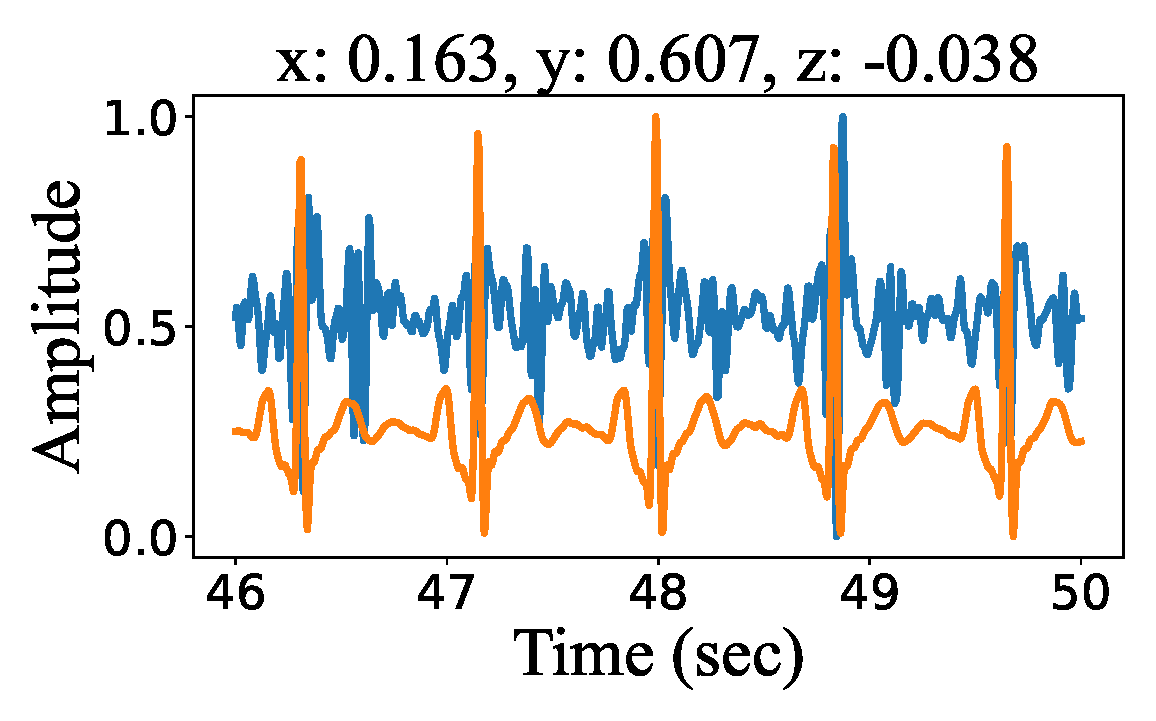
\includegraphics[width=0.35\columnwidth]{radar_good.eps}}
        \subfloat[]{\label{fig:radar_bad}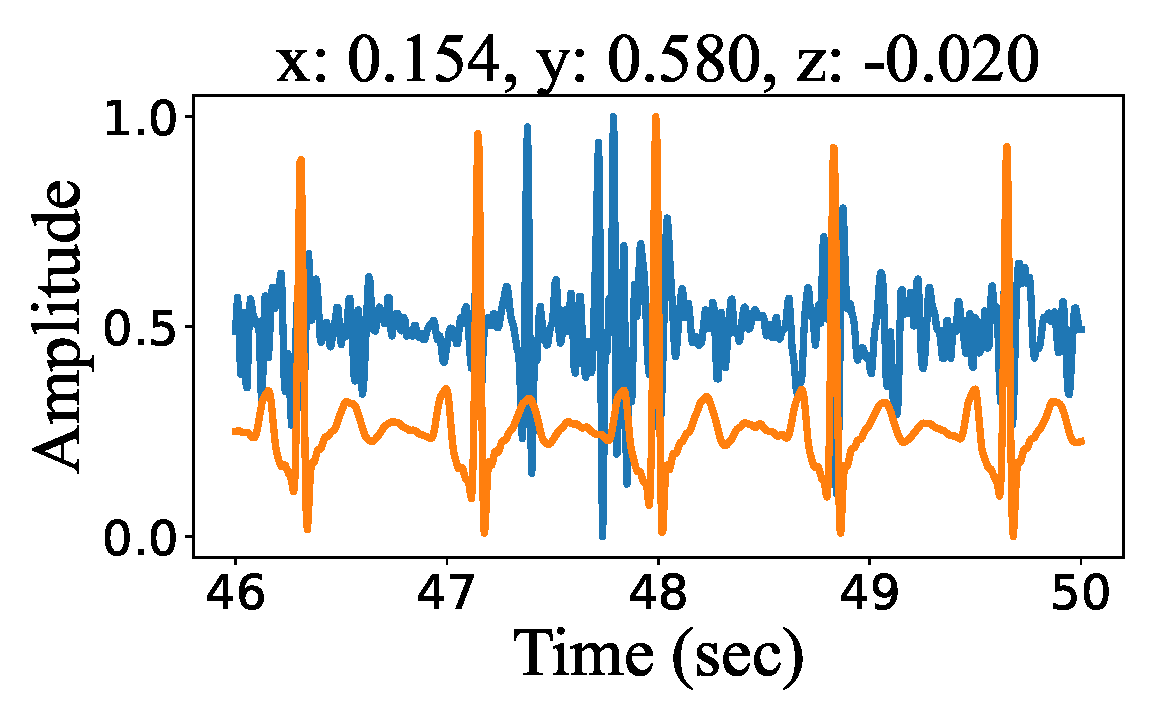
\includegraphics[width=0.35\columnwidth]{radar_bad.eps}} 
        \caption{Challenges for high-SNR signal collection: (a) and (b) Radar signals with high and low SNR for adjacent points with a distance of $0.03$m.}
        \label{fig:challenges}
\end{figure}
Based on the discussion Chapter~\ref{sec:the_first_challenge}, it is still a challenge to precisely locate and track the cardiac location during data collection to efficiently extract high-SNR radar signal. Although, it is natural to think the high-SNR radar signal can be searched in a constrained space by optimization, there is no appropriate method to assess the signal SNR in terms of cardiac features contained, and the objective space is actually highly discontinuous with adjacent points may revealing totally different SNR as shown in Figure~\subref*{fig:radar_good} and~\subref*{fig:radar_bad}, restricting the application of common gradient-based optimization algorithms. To address these issues, the contributions of this study can be listed as: 
\begin{itemize}
\item A \gls{cft} algorithm is proposed based on derivative-free optimization (DFO) to find the gls{cf} point by iteratively evaluating the potential points in a discontinuous objective space, with a universal signal template designed to adaptively assess the signal SNR as costs.
\item The proposed CFT algorithm has been validated on sitting subjects in various scenarios and could provide radar measurements with better SNR compared with existing methods.
\end{itemize}

The rest of this chapter is organized as follows. Section~\ref{sec:cftmethod} elaborates the proposed CFT algorithm, with the experimental settings and results shown in Section~\ref{sec:cftexp} and~\ref{sec:cftresult}. The final conclusion is shown in Section~\ref{sec:cftcon}.


\section{Methodology}\label{sec:cftmethod}
\subsection{Overview of CFT Algorithm for ECG Recovery}
The pipeline of using CFT algorithm is shown in Figure~\ref{fig:CFTRFcardi} with three steps:
\begin{itemize}
\item The received radar signal will be converted into a standard format in terms of chirp, frame and virtual antenna channel to obtain the general location of the subject, as shown in Figure~\ref{fig:CFTRFcardi}(a).
\item The rough location acts as the initial state for the CFT algorithm, and the points within a constrained space will be evaluated to find the red CF point with best SNR as shown in Figure~\ref{fig:CFTRFcardi}(b).
\item Signals extracted from the ten best points will be converted into spectrograms to train the deep learning model designed in~\cite{zhang2024radarODE-MTL} and generate corresponding ECG recoveries, as shown in Figure~\ref{fig:CFTRFcardi}(c).
\end{itemize}

In addition, TI-AWR 1843 radar operated at $77$~Ghz with $2$~Tx and $4$~Rx will be used for data collection, enabling $8$ virtual antenna channels for high-quality signal extraction. The detailed scenario descriptions and radar configurations will be provided in Section~\ref{sec:cftdata_coll}.

\begin{figure}[tb] 
    \centering 
    \includegraphics[width=0.99\columnwidth]{CF_Cardi_struct.pdf}
    \caption{Overview of using CFT for radar-based ECG covery: (a) Rough localization of human body; (b) Use CFT to find CF point and extract high-SNR radar signals; (c) Deep learning for ECG recovery.}
    \label{fig:CFTRFcardi} 
\end{figure}

\subsection{Rough Localization}
The received radar signal is first formatted as a standard data matrix in terms of different chirps, frames and virtual channels to provide measurement of range, velocity and AoA, respectively. For the current research level of radar-based vital sign monitoring, the subjects are all quasi-static without velocity, and only the range-angle (RA) map will be calculated using fast Fourier transform (FFT) as shown in Figure~\ref{fig:CFTRFcardi}(a), with a detailed illustration of signal waveform and processing shown in Figure~\ref{fig:rouch_loc}.

\subsubsection{Range FFT}
According to (\ref{equ:raw_sig}), the signal propagation after transmitting introduces a constant phase shift $\phi_s$ in the received signal and is expressed as 
\begin{equation}\label{equ:range}
\phi_s = \frac{4\pi d_0}{\lambda}
\end{equation}
with $d_0$ representing the distance between radar and human body. Therefore, the distance $d_0$ can be extracted from each received signal along fast time using FFT as shown in Figure~\ref{fig:rouch_loc}(a), and the updated data matrix now reveals the range information, i.e., a static object denoted as blue along slow time axis.
\begin{figure}[tb] 
    \centering 
    \includegraphics[width=0.9\columnwidth]{rough_loc.pdf}
    \caption{Procedures for obtaining RA map: (a) Range FFT for chirps along fast time; (b) Angle FFT along virtual channels.}
    \label{fig:rouch_loc} 
\end{figure}
\subsubsection{Angle FFT}
The ability of AoA detection relies on the MIMO system using time division multiplexing (TDM-MIMO), with multiple Tx alternately transmitting chirp signals and the corresponding reflections can be distinguished during receiving as shown in Figure~\ref{fig:rouch_loc}(b). Due to the physical distance varies for different Tx/Rx combinations (i.e., Tx$2$Rx$4$ creates $8$ virtual channels), an extra propagation $\Delta \phi_v$ delay will be introduced as:
\begin{equation}\label{equ:angle}
\begin{aligned}
\Delta \phi_v &= \frac{4\pi d_v}{\lambda} \\
d_v &= l\ sin(\theta)
\end{aligned}
\end{equation}
where $d_v$ represents the extra propagation distance, $l$ means the distance between adjacent antenna channels and $\theta$ is the incident angle. Similar to range FFT, the phase differences across different channels can be used to extract AoA information for each range bin by performing FFT along the channel axis, as shown in red squares in Figure~\ref{fig:rouch_loc}(b).

After combining the FFT results for all chirps and channels, the final RA map for the current time sample (frame) can be obtained as shown in Figure~\ref{fig:rouch_loc}. The same procedure can be repeated along the slow time axis to get the rough human body location for all the time samples, but this study only requires the location obtained from the very first frame as the initial point $E_0$ for CFT algorithm.

\subsection{Cardio-focusing and -tracking (CFT) Algorithm}
The radar signal for any point can be extracted following (\ref{equ:raw_sig}) and (\ref{equ:phase}), and the search progress from $E_0$ to the best point $E_{b}$ (i.e., CF point with high SNR) requires: (a) an appropriate metric to assess whether the radar signal contains wanted cardiac features; (b) an optimization method that is applicable to the discontinuous objective space based on the assessed SNR values as costs. 

\subsubsection{Template Design for Assessing SNR}
An explicit SNR can be calculated with the known “clean” signal, while the "clean" signal for vital signs normally reveals two prominent vibrations corresponding to the ventricular contraction and relaxation~\cite{zhang2024radarODE}, as shown in Figure~\subref*{fig:target_org}. However, considering the vibrations may have subtle differences due to different scenarios or radar configurations (e.g., noise figure and sampling frequency), a universal template $h_m$ is designed in this study to fit the envelope of the radar signal as: 
\begin{equation}
h_m (t) = a_1 \exp(-\frac{(t-b_1)^2}{2c_1^2}) + a_2 \exp(-\frac{(t-b_2)^2}{2c_2^2})
\end{equation}
with $a_1$, $a_2$ controlling the amplitudes of the peaks, $b_1$, $b_2$ determining the centers of the peaks and $c_1$, $c_2$ adjusting the width of the peaks. In practice, $a_1$ and $b_1$ will be fixed based on the dominant peaks detected as the red points in Figure~\subref*{fig:target_sig}, and other parameters are left to be determined as a simple curve fitting problem. Finally, the \gls{mse} between the radar signal envelope and the synthetic template is reckoned to be an assessment of signal SNR as shown in Figure~\subref*{fig:target_sig}, because fewer components could fit the designed template for low-SNR radar signal without obvious cardiac features, as shown in Figure~\subref*{fig:target_org_bad} and~\subref*{fig:target_sig_bad}.

\begin{figure}[tb]
  \centering
  \subfloat[]{\label{fig:target_org}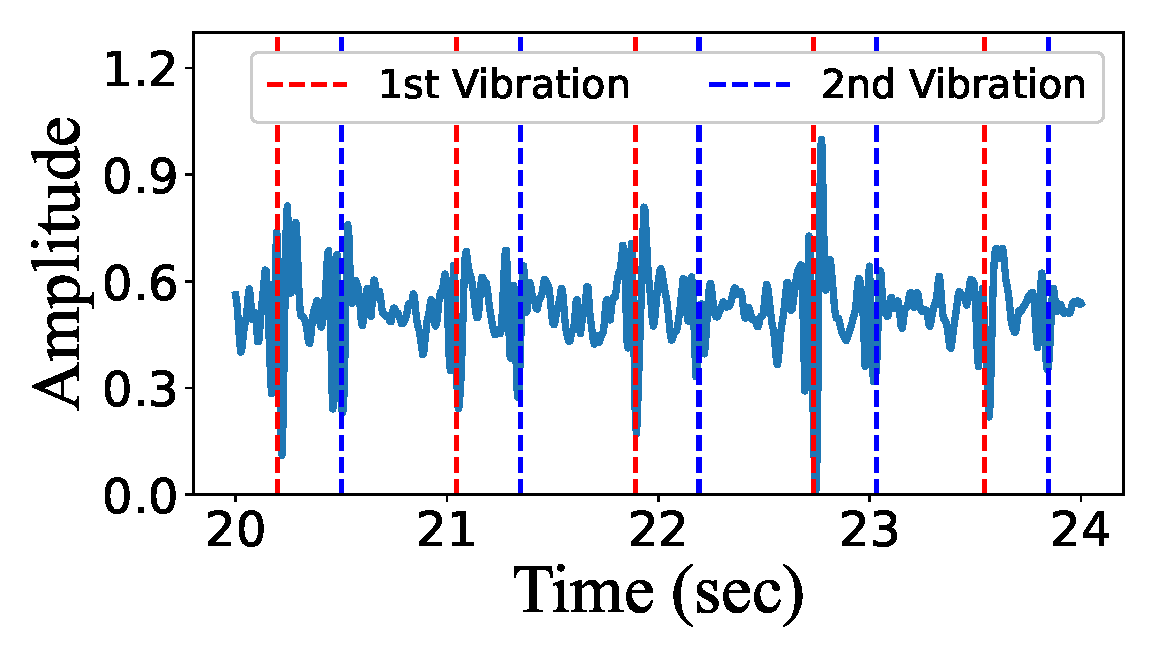
\includegraphics[width=0.4\columnwidth]{target_org.eps}}
  \subfloat[]{\label{fig:target_sig}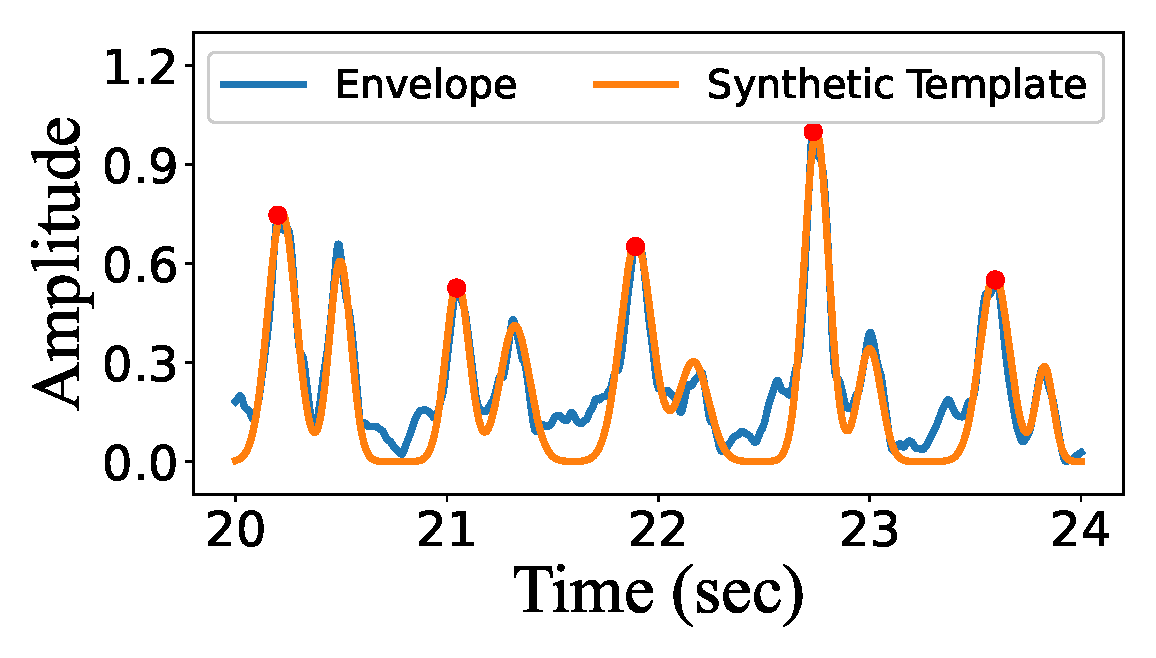
\includegraphics[width=0.4\columnwidth]{target_sig.eps}} \\
  \subfloat[]{\label{fig:target_org_bad}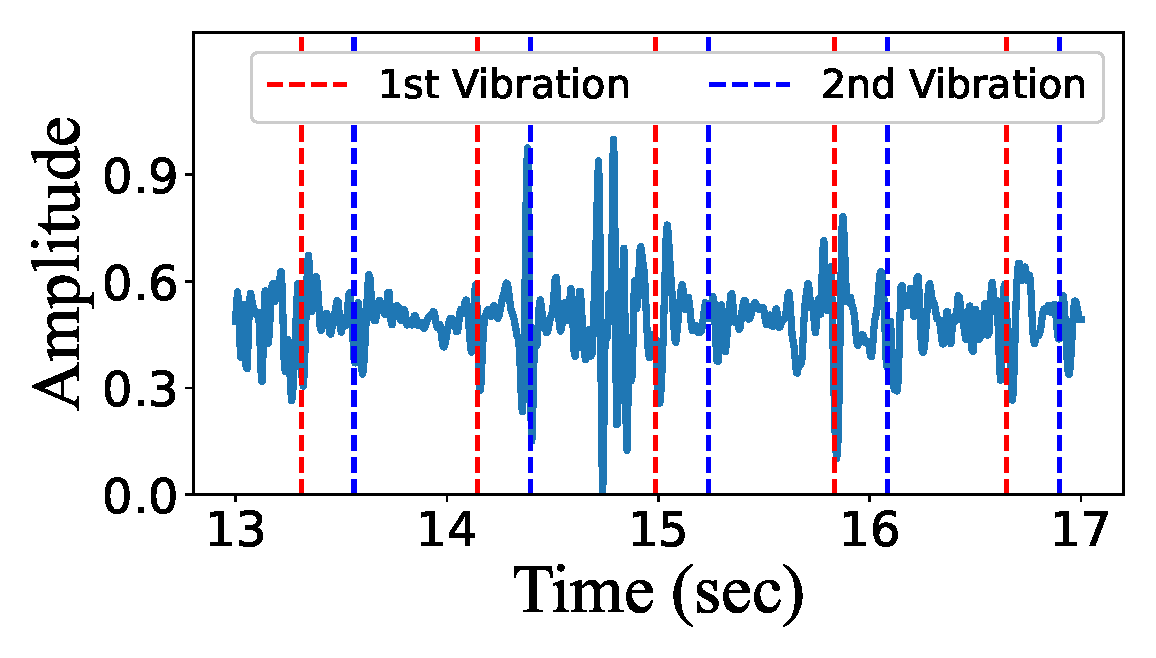
\includegraphics[width=0.4\columnwidth]{target_org_bad.eps}}
  \subfloat[]{\label{fig:target_sig_bad}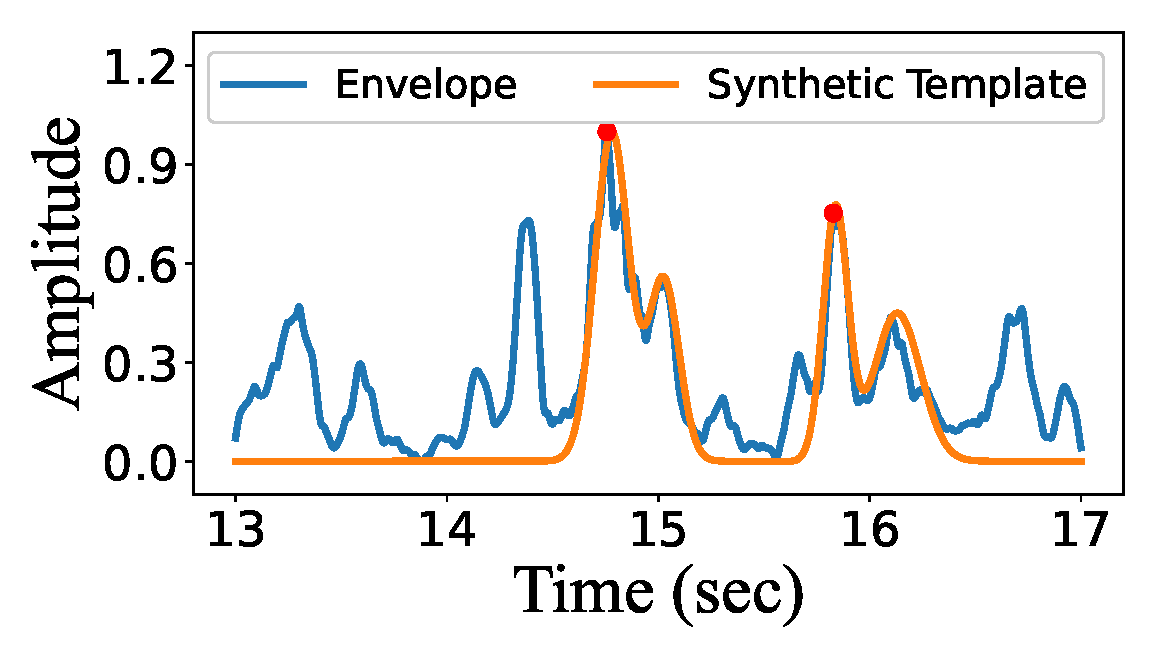
\includegraphics[width=0.4\columnwidth]{target_sig_bad.eps}}
  \caption{Template for assessing SNR: (a) High-SNR radar signal; (b) Extracted signal envelope with the synthetic template; (c) (a) Low-SNR radar signal, (d) Extracted signal envelope with the synthetic template.}
  \label{fig:template}
\end{figure}

\subsubsection{Derivative-free Optimization (DFO)}
The MSE values obtained from template matching for the radar pieces extracted from point $E$ will be used as costs $\mathcal{F}(E)$ in searching CF point, but the traditional gradient-based optimization method is not applicable because there is no explicit cost function. Therefore, the CFT algorithm is developed in a derivative-free manner based on coordinate search (CS) algorithm~\cite{larson2019derivative}, to asymptotically approach the CF point. 

The definition of the DFO problem is formulated as:
\begin{equation}
E_b = \underset{E \in \mathbb{R}^n}{\arg \min }\left\{\mathcal{F}(E) : E\in \Omega \right\}
\end{equation}
with $\Omega$ representing a user-defined constrained $n$-dimensional search space near initial point $E_0$ as shown in Figure~\ref{fig:CFTRFcardi}(b), and the cost of points out of the constraint will be set as $\mathcal{F}(E\not\in \Omega)=\infty$. During each iteration $k$, many trial points $E_k$ within the constraint will be evaluated to find the incumbent points $E_i$ as the temporary best point for the next iteration. 

To perform a derivative-free search, the traditional CS algorithm starts from the initialization of grids $G_k$:
\begin{equation}\label{equ:grid}
G_k := \{E_k + \gamma_kD\} \subset \mathbb{R}^n
\end{equation}
where $\gamma_k>0$ is the grid size parameter and $D$ contains several vectors $p$ for possible searching directions, as shown in Figure~\subref*{fig:cft_1}. The local convergence of CS is ensured by dense search directions $D$ and a refined grid size $\gamma_k$ to find better $E_i$ compared with current $E_k$~\cite{larson2019derivative}. However, the highly discontinuous objective space for radar-monitored vital signs may have numerous local minima that distract the optimization algorithm, i.e., the signal SNR of the adjacent points might be very different, as shown in Figure~\subref*{fig:radar_good} and~\subref*{fig:radar_bad}.

\begin{figure}[tb]
  \centering
  \begin{minipage}[t]{0.5\columnwidth}
  \subfloat[]{\label{fig:cft_1}\includegraphics[width=0.5\columnwidth]{cft_1.pdf}}\\
  \subfloat[]{\label{fig:cft_2}\includegraphics[width=0.5\columnwidth]{cft_2.pdf}}
  \end{minipage}%
  \hspace{-0.2\columnwidth}
  \begin{minipage}[t]{0.5\columnwidth}
  \vspace{0.08\columnwidth}
  \subfloat[]{\label{fig:cft_3}\includegraphics[width=1\columnwidth]{cft_3.pdf}}
  \end{minipage}%
  \caption{Illustration of the CFT algorithm with bold line wrapping the search region $S_k$: (a) Equality between $\gamma$ and $\Gamma$ (same as in CS algorithm); (b) Large $\Gamma_k$ with refined $\gamma_k$, providing more potential points to be evaluated; (c) Jump out of the local minimum by adjusting $\Gamma_k$ and $\gamma_k$.}
  \label{fig:cft_plot}
\end{figure}

To jump out of the potential local minimum, CFT algorithm is proposed by introducing search region $S_k$ to restrict the possible search directions $p$, alleviating the difficulty of searching in numerous dense grid points and allowing the adjustment of search region and grid size iteratively to break the local minimum. The detailed procedures of CFT are shown in Algorithm~\ref{alg:CFT}, with an illustration of $\mathbb{R}^2$ space shown in Figure~\ref{fig:cft_plot}. 

In CFT, the grids $G_k$ is still expressed as in (\ref{equ:grid}) and the newly introduced search region $S_k$ is expressed as:
\begin{equation}
S_k := \{E\in G_k : \| E-E_k \|_{\infty} \leq \Gamma_k a \}
\end{equation}
with $a=\max \left\{\left\|a^{\prime}\right\|_{\infty}: a^{\prime} \in D\right\}$ and $\Gamma_k$ as the size parameter for the search region. An intuitive interpretation of $S_k$ is the point set that contains grid points inside and on the boundary of the bold line controlled by $\Gamma_k$, as shown in Figure~\subref*{fig:cft_2}.

Based on the well-constructed grids $G_k$ and search region $S_k$, the remaining CFT algorithm is performed with searching and resizing stages:

\textbf{Searching: } The searching stage simply asks for the evaluation of $\mathcal{F}(E)$ on a subset of grids $G_k$ based on any sampling algorithm (e.g., Latin hypercube sampling~\cite{larson2019derivative}), as indicated in line~\ref{line:s1} in Algorithm~\ref{alg:CFT}.

\textbf{Resizing: } The resizing stage depends on the result of searching stage: 
\begin{itemize}
  \item If a new incumbent point $E_i$ is found with better SNR, the search region will be doubled as $\Gamma_{k+1}=2\Gamma_k$ (line~\ref{line:r1}), and the grid size will be empirically set as $\gamma_{k+1}=\min(\Gamma_k, {\Gamma_k}^2)$ (line~\ref{line:r4}), enabling to search in broader space in the next iteration.
  \item If there is no better point than the current $E_k$ on the current grids $G_k$, another searching stage will be performed only within the search region $S_k$ (line~\ref{line:s2}). Then, If a better point $E_i$ is found, $\Gamma_{k+1}$ and $\gamma_{k+1}$ is obtained as above (line~\ref{line:r2}), otherwise, the search region will be halved as $\Gamma_{k+1}=\Gamma_k/2$ (line~\ref{line:r3}) for a finer search with $\gamma_{k+1}=\min(\Gamma_k, {\Gamma_k}^2)$ (line~\ref{line:r4}).
\end{itemize}

The searching step enables the finding of better points $E_i$ in a broad space, and the resizing step either refines the grid if the current $\gamma_{k}$ is not enough or enlarges the search space when stalling at the local minimum, as shown in Figure~\subref*{fig:cft_3}. Finally, the CFT algorithm will be terminated after achieving a desired SNR$_d$ or iteration limit $k_{max}$.

\begin{algorithm}[tb]
\caption{CFT Algorithm}\label{alg:CFT}
\begin{algorithmic}[1]
    \State \textbf{Input:} $E_0$, SNR$_d$, $k_{max}$
    \State \textbf{Output:} $E_b$, SNR$_b$
    \Statex \textsc{Objective}:
    \State $E_b = \underset{E \in \mathbb{R}^n}{\arg \min }\left\{\mathcal{F}(E) : E\in \Omega \right\}$
    \State Initialize $k=0$, $\Gamma_k = \gamma_k = 1$, $SNR_b=\mathcal{F}(E_k)$
    \While {$SNR_b>SNR_d$ and $k<k_{max}$}
% \Statex \textsc{Searching}:
    \If{$\mathcal{F}(E)<SNR_b$ for some $E\in G_k$} \label{line:s1}
      \State $E_{k+1}\leftarrow E$, $SNR_b \leftarrow \mathcal{F}(E)$ 
      \State $\Gamma_{k+1}\leftarrow 2\Gamma_k$ \label{line:r1}
% \Statex \textsc{Resizing}:
% \Statex \textsc{Searching}:
    \ElsIf{$\mathcal{F}(E)<SNR_b$ for some $E\in S_k$} \label{line:s2}
% \Statex \textsc{Resizing}:
      \State $E_{k+1}\leftarrow E$, $SNR_b \leftarrow \mathcal{F}(E)$
      \State $\Gamma_{k+1}\leftarrow 2\Gamma_k$ \label{line:r2}
    \Else
      \State $E_{k+1} \leftarrow E_{k}$
      \State $\Gamma_{k+1}\leftarrow \Gamma_k/2$ \label{line:r3}
    \EndIf
    \State $\gamma_{k+1}\leftarrow \min(\Gamma_k, {\Gamma_k}^2)$ \label{line:r4}
    \State $k \leftarrow k+1$, $E_b \leftarrow E_{k+1}$
    \EndWhile
\end{algorithmic} 
\end{algorithm} 

The visualization of the CFT algorithm in Figure~\ref{fig:CFTRFcardi}(b) shows that initial iterations search in a large space, and the algorithm could jump out of the green local minima to find the red CF point within the fine blue grid points. In addition, the tracking of the CF points along time can be naturally realized by repeating Algorithm~\ref{alg:CFT} with previous $E_b$ as the new $E_0$, and the SNR evaluated on the previous point might have already achieved SNR$_d$ due to the quasi-static human body, saving a huge amount of time for calculating useless channel information for filtering or clustering~\cite{li2024radarnet,chen2022contactless,liu2024diversity}. 

\section{Details of Experiment and Dataset}\label{sec:cftexp}
\subsection{Dataset Collection and Preparation}\label{sec:cftdata_coll}
% \subsubsection{Dataset Collection and Preparation}
The dataset contains a total of $80$-minute synchronous radar-ECG pairs collected for $5$ healthy subjects ($3$ men, $2$ women) in $2$ indoor scenarios as shown in Figure~\ref{fig:data_col}. The subjects are asked to sit causally and are allowed to change postures during data collection, and each data trial lasts for $1$ minute. The distance between radar and human body varies from $0.5-1.2$m, and a longer distance causes the decrease of signal SNR with a smaller portion of the space points containing useful cardiac features. 

TI-AWR 1843 radar with $2$ Tx and $4$ Rx is used for data collection with $8$ virtual antenna channels created~\cite{AWR1843}, and the radar configurations are listed in Table~\ref{tab:data_param} with the name provided in TI mmWave-Studio interface. The signal will be sampled as $200$Hz, and only a band-pass filter from $0.5$ to $50$Hz and a differentiator are used for removing respiration noise because the radar signal extracted from CF points already has high SNR. Lastly, the ECG ground truth is collected using TI ADS1292, and the related ECG processing (e.g., smoothing and peak finding) is realized by NeuroKit2 python package~\cite{makowski2021neurokit2}.

\begin{figure}[tb]
  \centering
  \includegraphics[width=0.8\columnwidth]{scen_1.pdf}
  \caption{Indoor scenarios for data collection.}
  \label{fig:data_col}
\end{figure}

\begin{table}[tb]
\centering
\caption{Parameters for data collection interface}
    \begin{tabular}{lc?lc}
    \toprule
    \textbf{Parameter} & \textbf{Value} & \textbf{Parameter} & \textbf{Value} \\
    \toprule
    Start Frequency & $77$GHz & Frequency Slope & $65$MHz/$\mu$s \\ 
    Idle Time & $10\mu$s    & Tx Start Time & $1\mu$s \\
    ADC Start Time & $6\mu$s  & ADC Samples & $256$ \\ 
    Sample Rate & $5000$kbps  & Ramp End Time & $60\mu$s \\ 
    % Rx Gain & $30$ dB  & Rx Gain Target & $30$ dB  \\ 
    Start/End Chirp Tx & $0/2$  & No. of Chirp Loops & $2$  \\ 
    No. of Frames & $12000$  & Frame Periodicity & $5$ms  \\ 
    \bottomrule
    \end{tabular}
\label{tab:data_param}
\end{table}%

\subsection{Implementation Details}
\subsubsection{Parameters for CFT Algorithm}
The constraint $\Omega$ for the CF point search is centered at the initial state $E_0$ with a range of $0.4\times 0.2 \times 0.4$m as illustrated in Figure~\ref{fig:CFTRFcardi}(b). In addition, the initial grid and search region size should be adjusted to fit the real-life physical unit as $\Gamma_k= \gamma_k = 0.1$m, and the size will be limited as $\Gamma_k\geq\gamma_k\geq 0.001$m to prevent an exhaustive search within a meaningless small space. At last, SNR$_d$ is set to $0.01$ for the desired MSE between normalized synthetic template and signal envelope, and $k_{max}$ is set to $100$.

\subsubsection{Deep Learning Model Training}
The deep learning model adopts the same backbone, ECG decoder and hyperparameters as in our previous open-sourced work~\cite{zhang2024radarODE-MTL} coded in PyTorch and trained on NVIDIA RTX 4090 (24GB). The total training epoch is set to $100$ with batch size $8$, and a $5$-fold cross-validation training strategy is adopted to split the dataset to make the most of the limited dataset while excluding the testing data from the training phase.


\subsection{Methods for Comparison}
The comparison is performed with the representative methods based on accumulation and clustering to extract high-SNR radar signal:
\begin{itemize}
  \item De-ViMo~\cite{liu2024diversity} is proposed for heart rate monitoring and is based on the accumulation of signals from various dimensions (e.g., chirps, antennas, spatial points) to enhance cardiac features while mitigating noise. In addition, De-ViMo also improves the rough localization by identifying the peaks in micro-motion frequency bands instead of the entire FMCW bands.
  \item MMECG~\cite{chen2022contactless} requires the calculation of numerous points in 3D space and applies clustering algorithm to improve SNR. Then, a pattern-matching process is performed to learn the common pattern from the clustered result and select the best radar signal(s).
\end{itemize}

\begin{figure*}[tbp]
  \centering
  \begin{minipage}{0.1\linewidth}\centering\scriptsize
\rotatebox[origin=center]{0}{\textbf{Rough Loc.}}
\rotatebox[origin=center]{0}{$\approx$}\\
\rotatebox[origin=center]{0}{\textbf{CF Point}}
\end{minipage}\begin{minipage}{0.9\linewidth}\centering
  \subfloat[]{\label{fig:bf_good}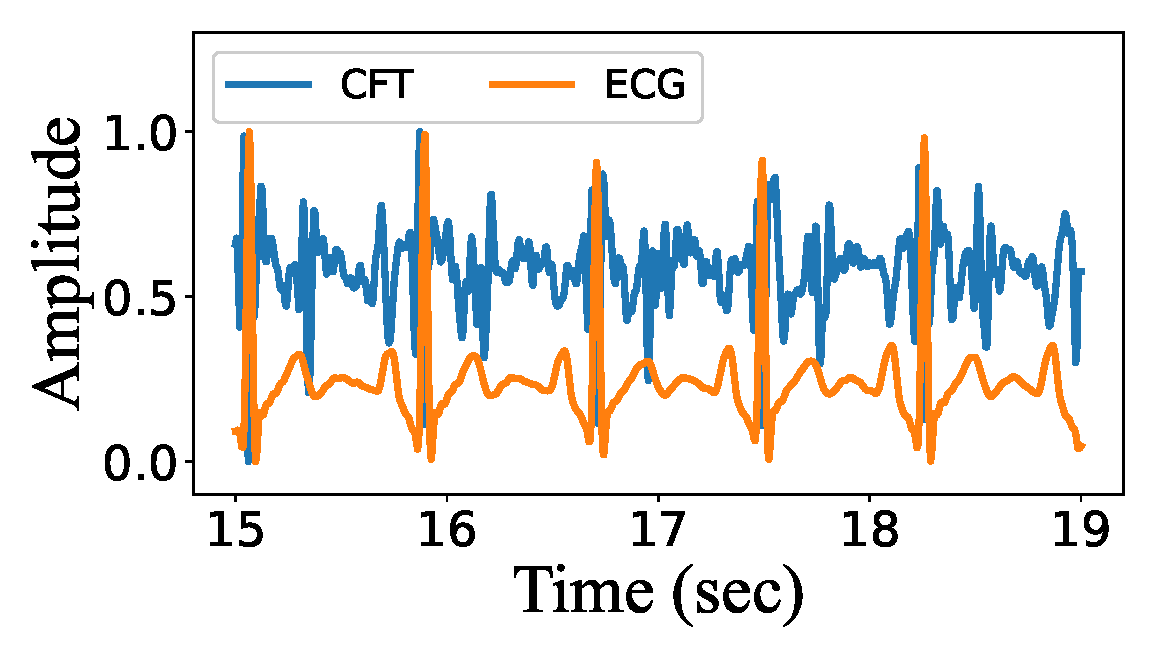
\includegraphics[width=0.3\columnwidth]{bf_good.eps}}
  \subfloat[]{\label{fig:MMECG_good}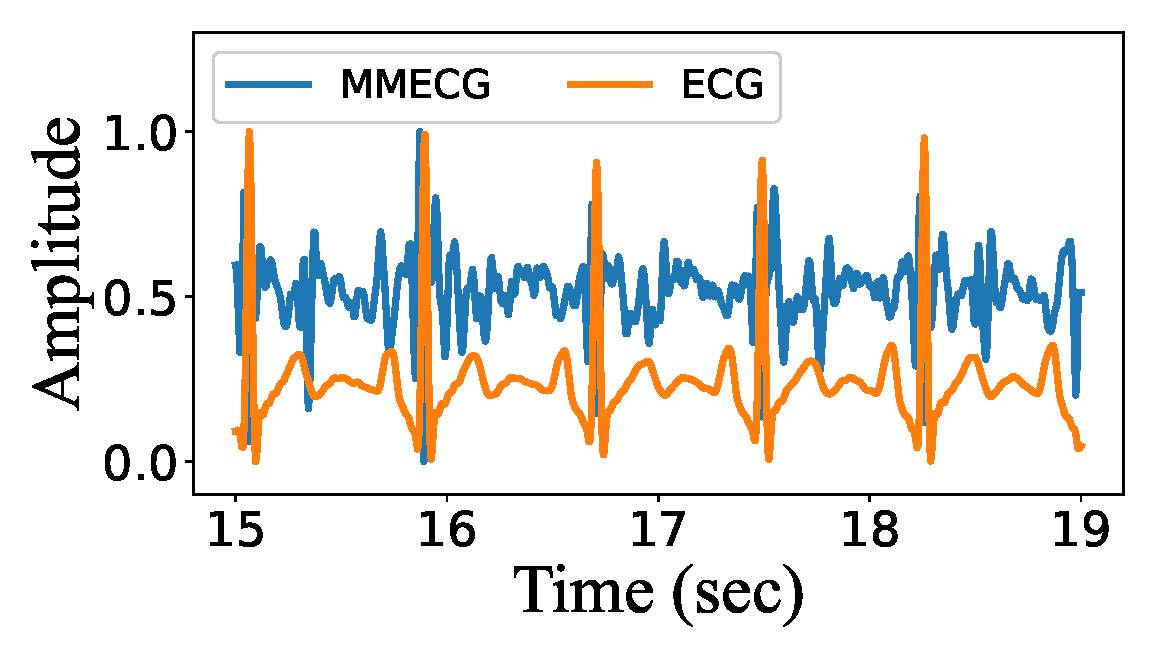
\includegraphics[width=0.3\columnwidth]{mmecg_good.eps}}
  \subfloat[]{\label{fig:vimo_good}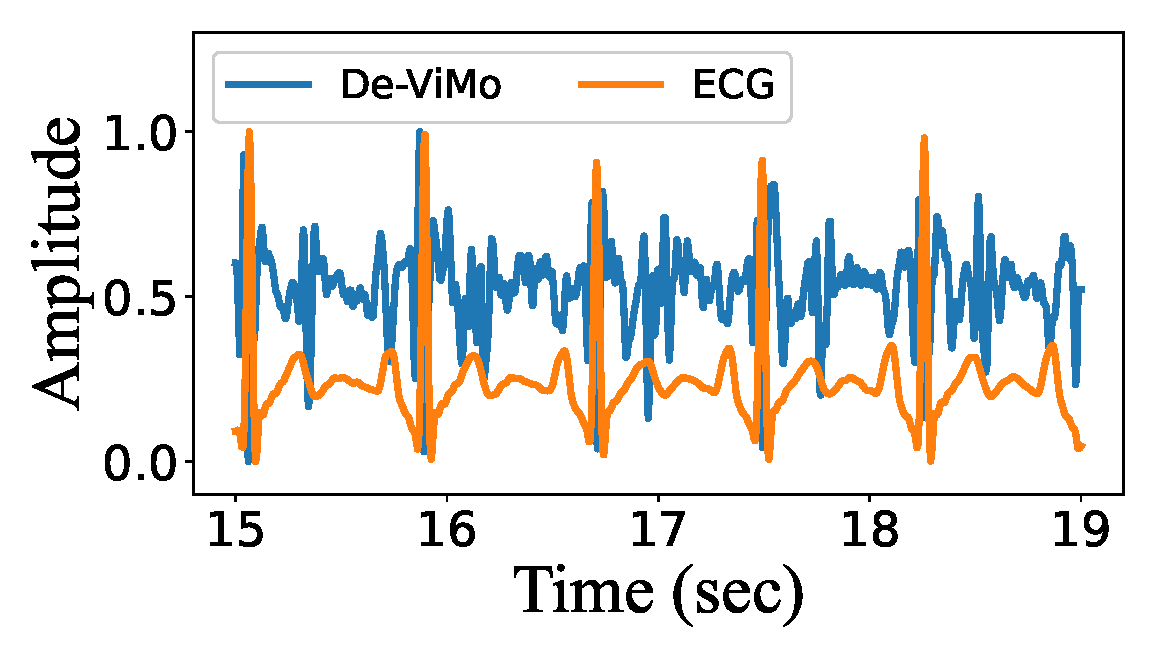
\includegraphics[width=0.3\columnwidth]{devimo_good.eps}}\\
\end{minipage}
\begin{minipage}{0.1\linewidth}\centering\scriptsize
\rotatebox[origin=center]{0}{\textbf{Rough Loc.}}
\rotatebox[origin=center]{0}{$\neq$}\\
\rotatebox[origin=center]{0}{\textbf{CF Point}}
\end{minipage}\begin{minipage}{0.9\linewidth}\centering
  \subfloat[]{\label{fig:bf_bad}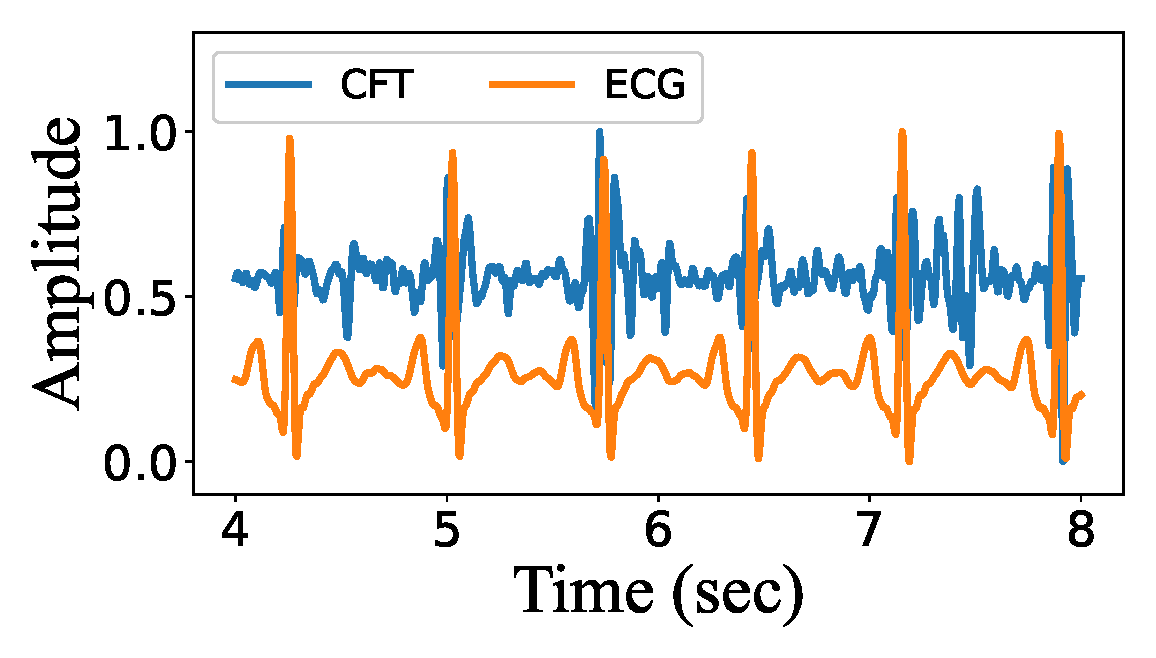
\includegraphics[width=0.3\columnwidth]{bf_bad.eps}}
  \subfloat[]{\label{fig:MMECG_bad}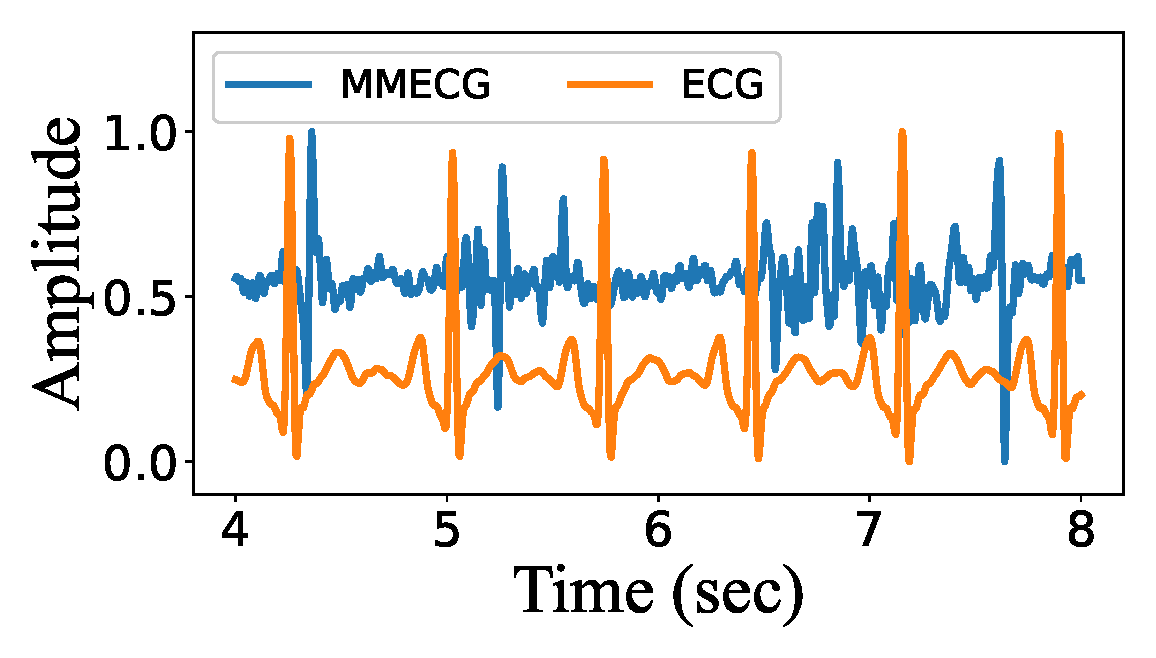
\includegraphics[width=0.3\columnwidth]{mmecg_bad.eps}}
  \subfloat[]{\label{fig:vimo_bad}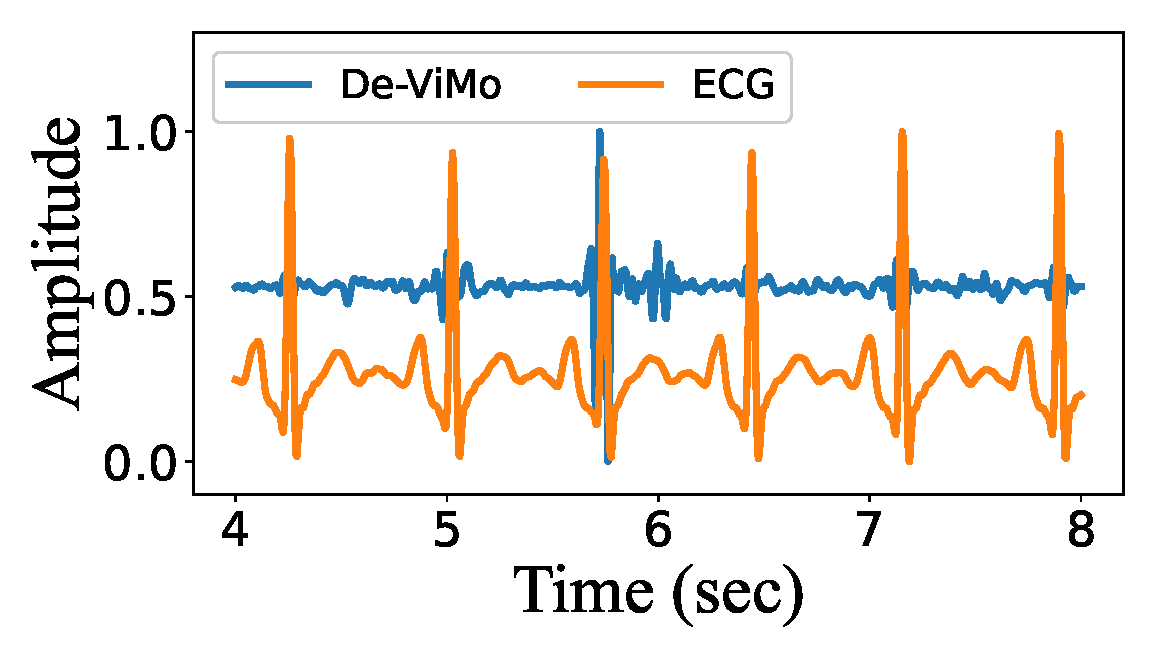
\includegraphics[width=0.3\columnwidth]{devimo_bad.eps}}
\end{minipage}
  \caption{Visualization of the extracted radar signal for all methods: (a) - (c) If CF point is around rough body location; (d) - (f) If CF point is far from rough body location.}
  \label{fig:compare_overall}
\end{figure*}

\section{Experimental Results and Evaluations}\label{sec:cftresult}
\subsection{Effectiveness of CFT Algorithm}
The examples of the extracted radar signal for different methods are shown in Figure~\ref{fig:compare_overall}, illustrating that precise cardiac localization has a huge effect on the signal quality. For example, if the rough body location is around CF point, all three methods can obtain high-SNR signals with clear first and second vibrations using either space search (CFT, Figure~\subref*{fig:bf_good}), clustering (MMECG, Figure~\subref*{fig:MMECG_good}) or accumulation (De-ViMo, Figure~\subref*{fig:vimo_good}). 

In contrast, only a few range bins will contain useful cardiac features if the rough body location is far from CF points, especially when increasing the monitoring range. Therefore, the signal accumulation may enhance the noises as shown in Figure~\subref*{fig:vimo_bad} while the signal clustering may also encounter a failure due to the lack of homogeneous cardiac signals as shown in Figure~\subref*{fig:MMECG_bad}. However, The proposed CFT could precisely locate the CF point with good SNR subject to the designed signal template and DFO searching strategy, and the extracted radar signal still shows clear peaks as shown in Figure~\subref*{fig:bf_bad}.

During the data collection of this study, the subjects are allowed to change postures to alleviate discomfort, with a resultant CF point deviation of several decimeters, while the rough location provided by FMCW signal processing is still unchanged. Therefore, the proposed CFT algorithm is essential because the posture change is inevitable, and a thorough evaluation in terms of different monitoring ranges will be performed in the next part.
\begin{figure}[tb]
  \centering
  \subfloat[]{\label{fig:pk_err_point}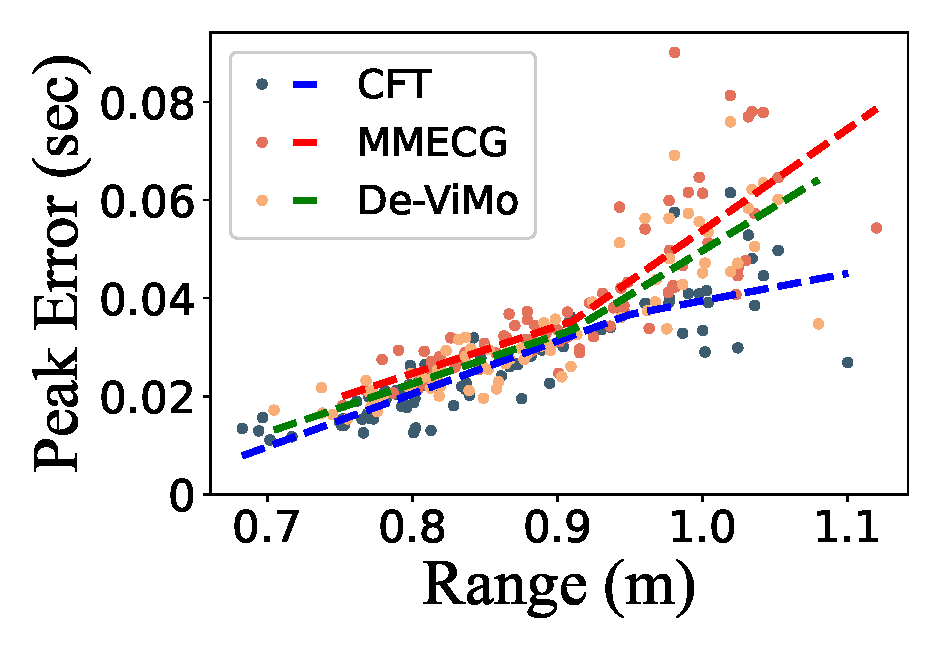
\includegraphics[width=0.35\columnwidth]{pk_err_point.eps}}
  \subfloat[]{\label{fig:pk_mdr_point}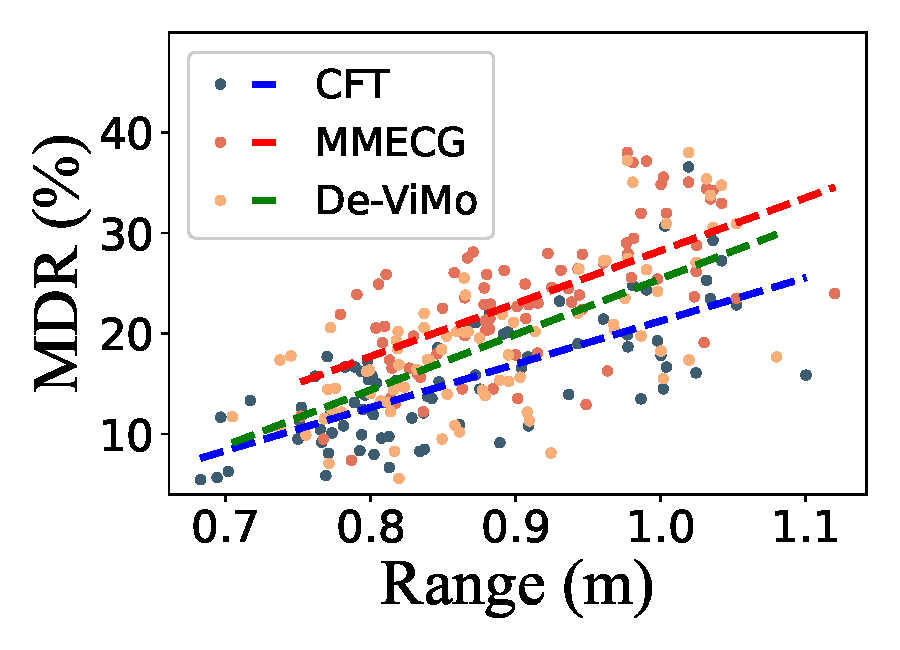
\includegraphics[width=0.34\columnwidth]{pk_mdr_point.eps}} \\
  \subfloat[]{\label{fig:pk_err_cdf}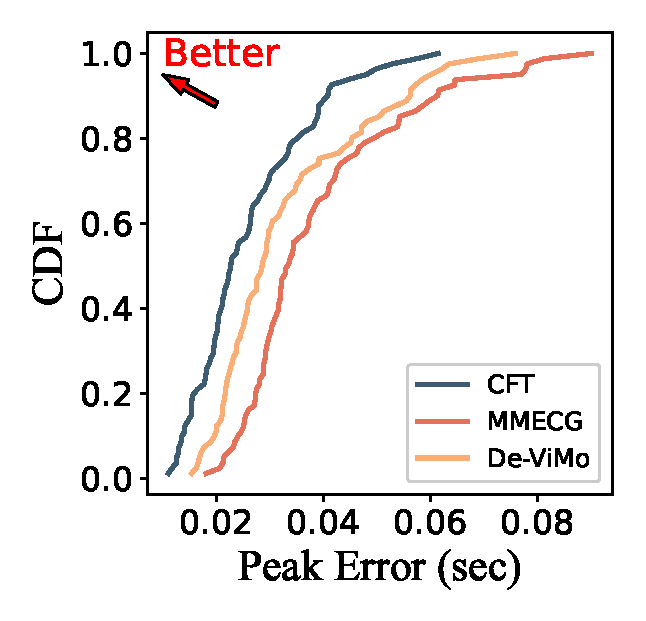
\includegraphics[width=0.35\columnwidth]{pk_err_cdf.eps}}
  \subfloat[]{\label{fig:pk_mdr_cdf}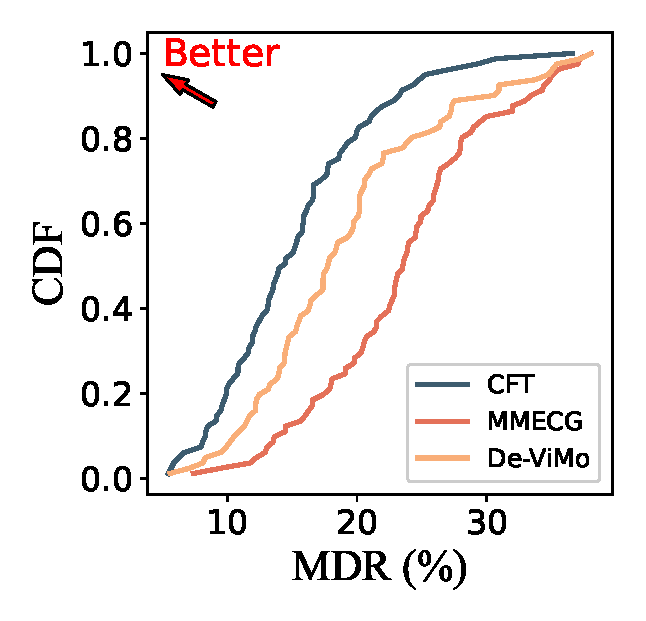
\includegraphics[width=0.35\columnwidth]{pk_mdr_cdf.eps}} 
  \caption{Illustration of performance in terms of peak error and MDR: (a) - (b) Scattered points with fitting curves along range axis; (c) - (d) CDF plots for all trails.}
  \label{fig:range_impact}
\end{figure}
\subsection{Impact of Monitoring Range}
To evaluate the performance of different methods when increasing the monitoring range, the quality of extracted radar signals for all trials is evaluated in terms of:
\begin{itemize}
\item Absolute Peak error between ECG R peaks and the dominant peaks for the first vibrations in radar signal.
\item \Gls{mdr} to count the cardiac cycles with no peak detected or with the absolute peak error larger than $150$ms~\cite{chen2022contactless}.
\end{itemize}

Figure~\subref*{fig:pk_err_point} and~\subref*{fig:pk_mdr_point} illustrate the peak error and MDR for all $80$ trials with corresponding fitting curves indicating the mean peak error or MDR. All the methods show similar performance in the short range and experience certain degradation with respect to the increasing range. In particular, MMECG shows larger degradation and variance for longer-range cases because the rough localization based on FMCW signal processing cannot provide accurate cardiac location, and the resultant evaluated points may not capture useful information for clustering. In contrast, De-ViMo could provide a better cardiac location, and the accumulated results show better accuracy than MMECG, while the long-range monitoring still affects the quality because the accumulation is not robust to non-gaussian noise. At last, the proposed CFT could precisely focus on the CF point and keep tracking the high-SNR points during data collection, providing the best results with small variance for both peak error and MDR. 

In addition, the \gls{cdf} plots for all trials are shown in Figure~\subref*{fig:pk_err_cdf} and~\subref*{fig:pk_mdr_cdf}. The proposed CFT algorithm achieves the best peak error with a median value of $0.022$~sec, while DE-ViMo and MMECG have worse performances with larger median values of $0.028$~sec and $0.033$~sec, respectively. Similarly, the precise localization and tracking of CF point also reduces the MDR for CFT results with a median value of $14\%$, while DE-ViMo and MMECG may affected by the accumulated noise or inaccurate cardiac localization with the median MDR of $17\%$ and $23\%$, respectively.


\subsection{Impact of Signal Quality on ECG Recovery}
The signals extracted using different methods are used for supervised training to verify the impact of different input qualities on the ECG recovery task. The quality of the recovered ECG signal is assessed in terms of:
\begin{itemize}
\item The morphological accuracy is measured using MSE and \Gls{pcc}, with MSE sensitive to the peak deviation and PCC focusing on the similarity between the ECG patterns.
\item The accurate recovery of ECG R peaks is crucial to coarse cardiac features calculation (e.g., heart rate variability) and is measured by absolute R peak error and MDR.
\end{itemize}
Table~\ref{tab:ecg_supervise} shows the performance of the deep learning model trained with datasets yielded by different methods. The training based on CFT dataset achieves the best results on both morphological accuracy (MSE$=0.0082$ and PCC$=85.47\%$) and R peak recovery (Peak Error$=7.61$ms and MDR$=6.85\%$), because the high-SNR inputs provide accurate peak locations with minor noise that affects the ECG pattern generation, as shown in Figure~\subref*{fig:radar_clean} and~\subref*{fig:ecg_pred_clean}. 

\begin{table}[tb]
\centering
\caption{Performance of supervised ECG recovery}
    \begin{tabular}{c |cccc}
    \toprule
    Methods  & \makecell[c]{MSE ($\times 10^{-2}$)} $\downarrow$ & PCC $\uparrow$ & \makecell[c]{Peak Error (ms)} $\downarrow$ & MDR $\downarrow$ \\
    \toprule
    MMECG~\cite{chen2022contactless} & $0.93$  & $80.36\%$ & $9.74$ & $7.96\%$ \\
    De-ViMo~\cite{liu2024diversity} & $0.88$ & $83.83\%$ & $8.93$ & $7.32\%$\\
    \midrule
    CFT  &  $\mathbf{0.82}$ & $\mathbf{85.47\%}$ & $\mathbf{7.61}$ & $\mathbf{6.85\%}$\\
    \bottomrule
    \end{tabular}%
\label{tab:ecg_supervise}
\end{table}%

In contrast, MMECG and De-ViMo cannot preserve the signal quality especially for long-distance cases, and the noisy inputs will prevent the deep learning mode from identifying the accurate position of ECG pieces, causing large peak error and MDR, as shown in Figure~\subref*{fig:radar_noise} and~\subref*{fig:ecg_pred_noise}. It is worth noticing that poor signal SNR causes more degradation in peak error than morphological accuracy, because the ECG patterns share a similar shape and can be learned from other cardiac cycles, while the peak recovery (detection) fully relies on the current radar input and can be ruined by noises.

\begin{figure}[tb]
  \centering
  \subfloat[]{\label{fig:radar_clean}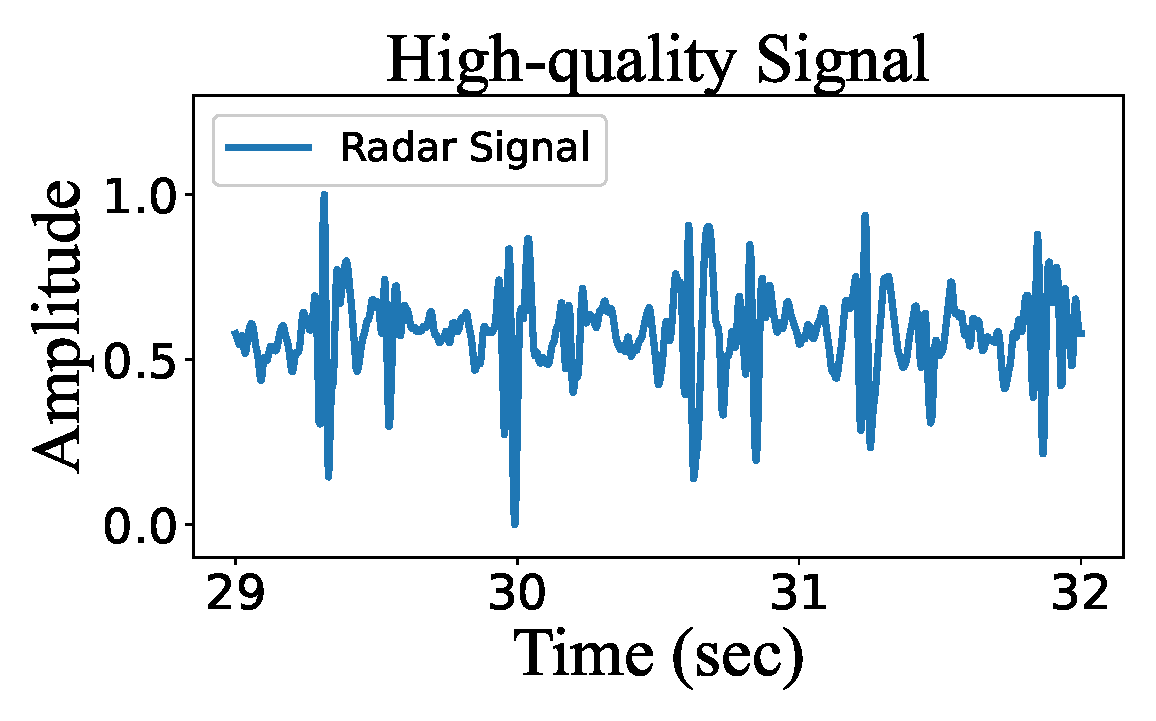
\includegraphics[width=0.4\columnwidth]{radar_clean.eps}}
  \subfloat[]{\label{fig:ecg_pred_clean}\includegraphics[width=0.4\columnwidth]{ecg_pred_clean.eps}} \\
  \subfloat[]{\label{fig:radar_noise}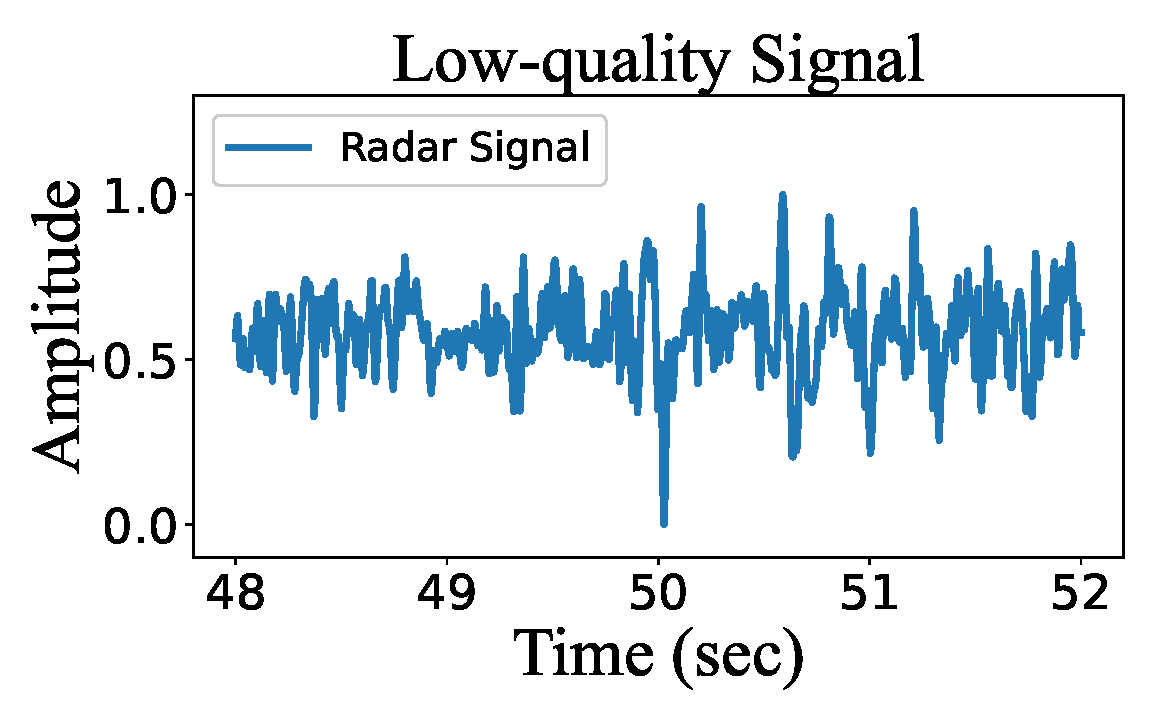
\includegraphics[width=0.4\columnwidth]{radar_noise.eps}}
  \subfloat[]{\label{fig:ecg_pred_noise}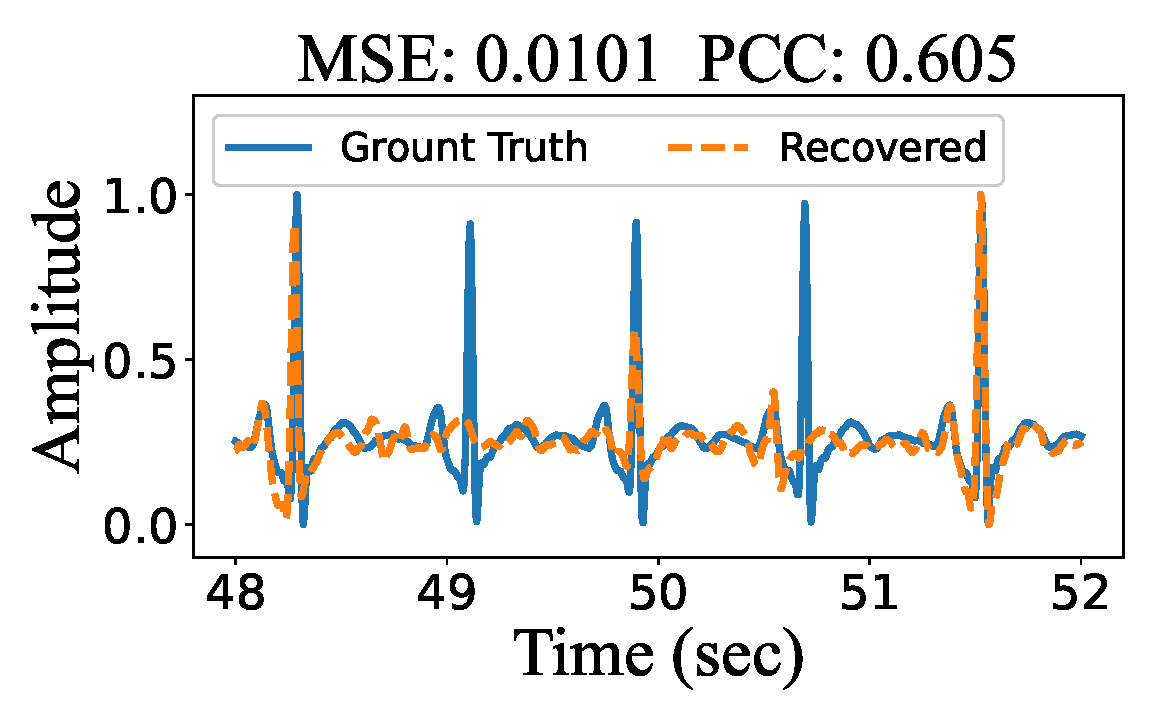
\includegraphics[width=0.4\columnwidth]{ecg_pred_noise.eps}} 
  \caption{Impact of radar input quality on the final ECG recovery: (a) - (b) High-quality radar input and ECG recovery; (c) - (d) Low-quality radar input and ECG recovery.}
  \label{fig:ecg_recovery}
\end{figure}

\section{Conclusions}\label{sec:cftcon}
This chapter investigates the efficient collection of high-SNR radar signals with ample cardiac features for deep-learning-based ECG recovery. Previous methods adopted signal accumulation or clustering to suppress the noises, while the rough localization based on FMCW radar cannot accurately reveal the chest region, requiring a time-consuming traverse among a 3D space for compensation. In this chapter, a novel CFT algorithm is proposed to dynamically articulate the points with the best SNR and could track the cardiac location over time if the subjects change posture. The experiments performed in different scenarios prove the feasibility of the CFT algorithm in radar signal collection for ECG recovery, enabling a convenient deployment in new scenarios for future contactless wellness monitoring.

\glsresetall
\chapter{Robust Single-Cycle ECG Generation}\label{ch:radarODE}
This chapter is based on the high-SNR radar measurements that contain ample cardiac features and aim to realize the robust ECG recovery to resist inevitable noises (e.g., \gls{rbm} noise). Previous studies leverage the powerful fitting capability of the \gls{dnn} to model complex and non-linear projections from radar to ECG signal, but the inference results can be easily distorted under abrupt noises~\cite{chen2022contactless,zhao2024airecg,zhao2024mmarrhythmia}. In this chapter, the traditional DNN is integrated with \gls{ode} with prior morphological features that constrain the ECG recovery, and a signal model is also designed to explain the critical features in the transformation from radar to ECG signals. The proposed ODE-embedded deep learning model is validated on the dataset with RBM noise, and the recovered ECG pieces still show high fidelity even when the subtle cardiac features are ruined by the noises with large amplitude.

\section{Introduction}
In the recent research about cardiac monitoring, the emergence of commercial radar platforms with high operating frequency encourages researchers to extract fine-grained cardiac features (e.g., ECG and SCG) from the radar signal~\cite{zhang2023overview}. SCG signal is measured by the accelerometer mounted on the human chest to measure the mechanical vibrations produced by heartbeats, describing the fine-grained cardiac mechanical activities such as aortic/mitral valve opening/closing and isovolumetric contraction~\cite{cocconcelli2020high}. Although these vibrations are subtle, it is still reasonable to directly map the displacements detected by radar to each fine-grained cardiac mechanical activity using high-resolution radar as proved in~\cite{ha2020contactless}. However, radar-based SCG recovery is not widely investigated compared with ECG, because ECG provides more comprehensive information (e.g., atrial/ventricular depolarization~\cite{khairy2007clinical}) for clinical diagnosis.

To reconstruct ECG from radar signal, the most straightforward approach is to directly sense the variation in the scattered electromagnetic field through frequency shift of mm-wave response, and the ECG signal can then be decoupled from the scattered electromagnetic field based on the dynamic model in the form of partial differential equations deduced from cardiac electrophysiology (i.e., ionic concentration in cardiac cells)~\cite{xu2021cardiacwave}. However, the solutions of the entire model are extremely hard to obtain either numerically or analytically, and the constructed models will be changed with respect to different environments and noises due to the Green's function~\cite{li2019intelligent}, causing difficulty in adapting the model in various real-life scenarios. 

The second approach, which is also the most adopted approach, only uses radar to sense the chest region displacement through the reflected radar signal as in coarse cardiac monitoring, but then the researchers must deal with domain decoupling to transform the measured signal from the mechanical domain to the electrical domain to generate ECG measurement. Intuitively, it is reasonable that mechanical conduction and electrical conduction are highly correlated in describing cardiac activities because the electrical changes in cells trigger heart muscle contraction, whereas such a relationship is called excitation-contraction coupling in electrophysiology and is extremely hard to interpret or model by researchers without biological knowledge~\cite{swift2021stop,orkand1964heart}.

In the literature, the existing studies all leverage deep learning methods to extract latent information from enormous radar/ECG pairs and try to learn domain transformation relying on the extraordinary non-linear mapping ability of the deep neural network~\cite{chen2022contactless,wu2023contactless,li2024radarnet,wang2023ecg,zhao2024airecg}. Although these studies could successfully reconstruct the ECG signal from radar, three drawbacks still need to be improved:
\begin{itemize}
    \item There is no existing signal model with a compact form to describe the domain transformation for radar-based ECG reconstruction.
    \item The purely data-driven method could learn the domain transformation as a black box, but researchers can hardly intervene in the learning process to enhance the characteristic peaks of ECG or explain the intrinsic correspondence in domain transformation.
    \item The well-trained deep learning model is not robust to abrupt noises such as body movement~\cite{chen2022contactless,wang2023vital}, because these noises normally have orders of magnitude higher than cardiac-related vibrations, drowning out subtle features and ruining forward propagation of the deep neural network~\cite{wang2023slprof}.
\end{itemize}

Inspired by the above discussions, this chapter aims to design a framework for radar-based ECG reconstruction with ordinary differential equations (ODEs) embedded to provide prior knowledge on domain transformation and resist abrupt noises. The contributions of this research can be concluded as:
\begin{itemize}
    \item This study proposes an ODE-embedded framework called radarODE to produce robust long-term ECG recovery against abrupt noises with the aid of morphological ECG features as the reference.
    \item A signal model is designed to describe the fine-grained cardiac feature sensed by radar, enabling further domain transformation between cardiac mechanical and electrical activities, instead of using purely data-driven approaches without any explanation as in the literature.
    \item Based on the proposed signal model, an ODE-embedded module called \gls{sceg} is designed to realize the domain transformation by parameterizing the radar signal into sparse representations and hence generate the morphological ECG features as references to resist noise.
\end{itemize}

The rest of the chapter is organized as follows. Section~\ref{sec:odemethod} explains the proposed model for radar signal and the structure of radarODE framework. Section~\ref{sec:odeexp} and~\ref{sec:odedataset} introduce the public dataset used for validation in this research and then present the results obtained with corresponding comparisons and evaluations. Finally, Section~\ref{sec:odeconclusions} concludes this chapter. 

\section{Methodology}\label{sec:odemethod}
\subsection{Overview}
\begin{figure*}[tb] 
    \centering 
    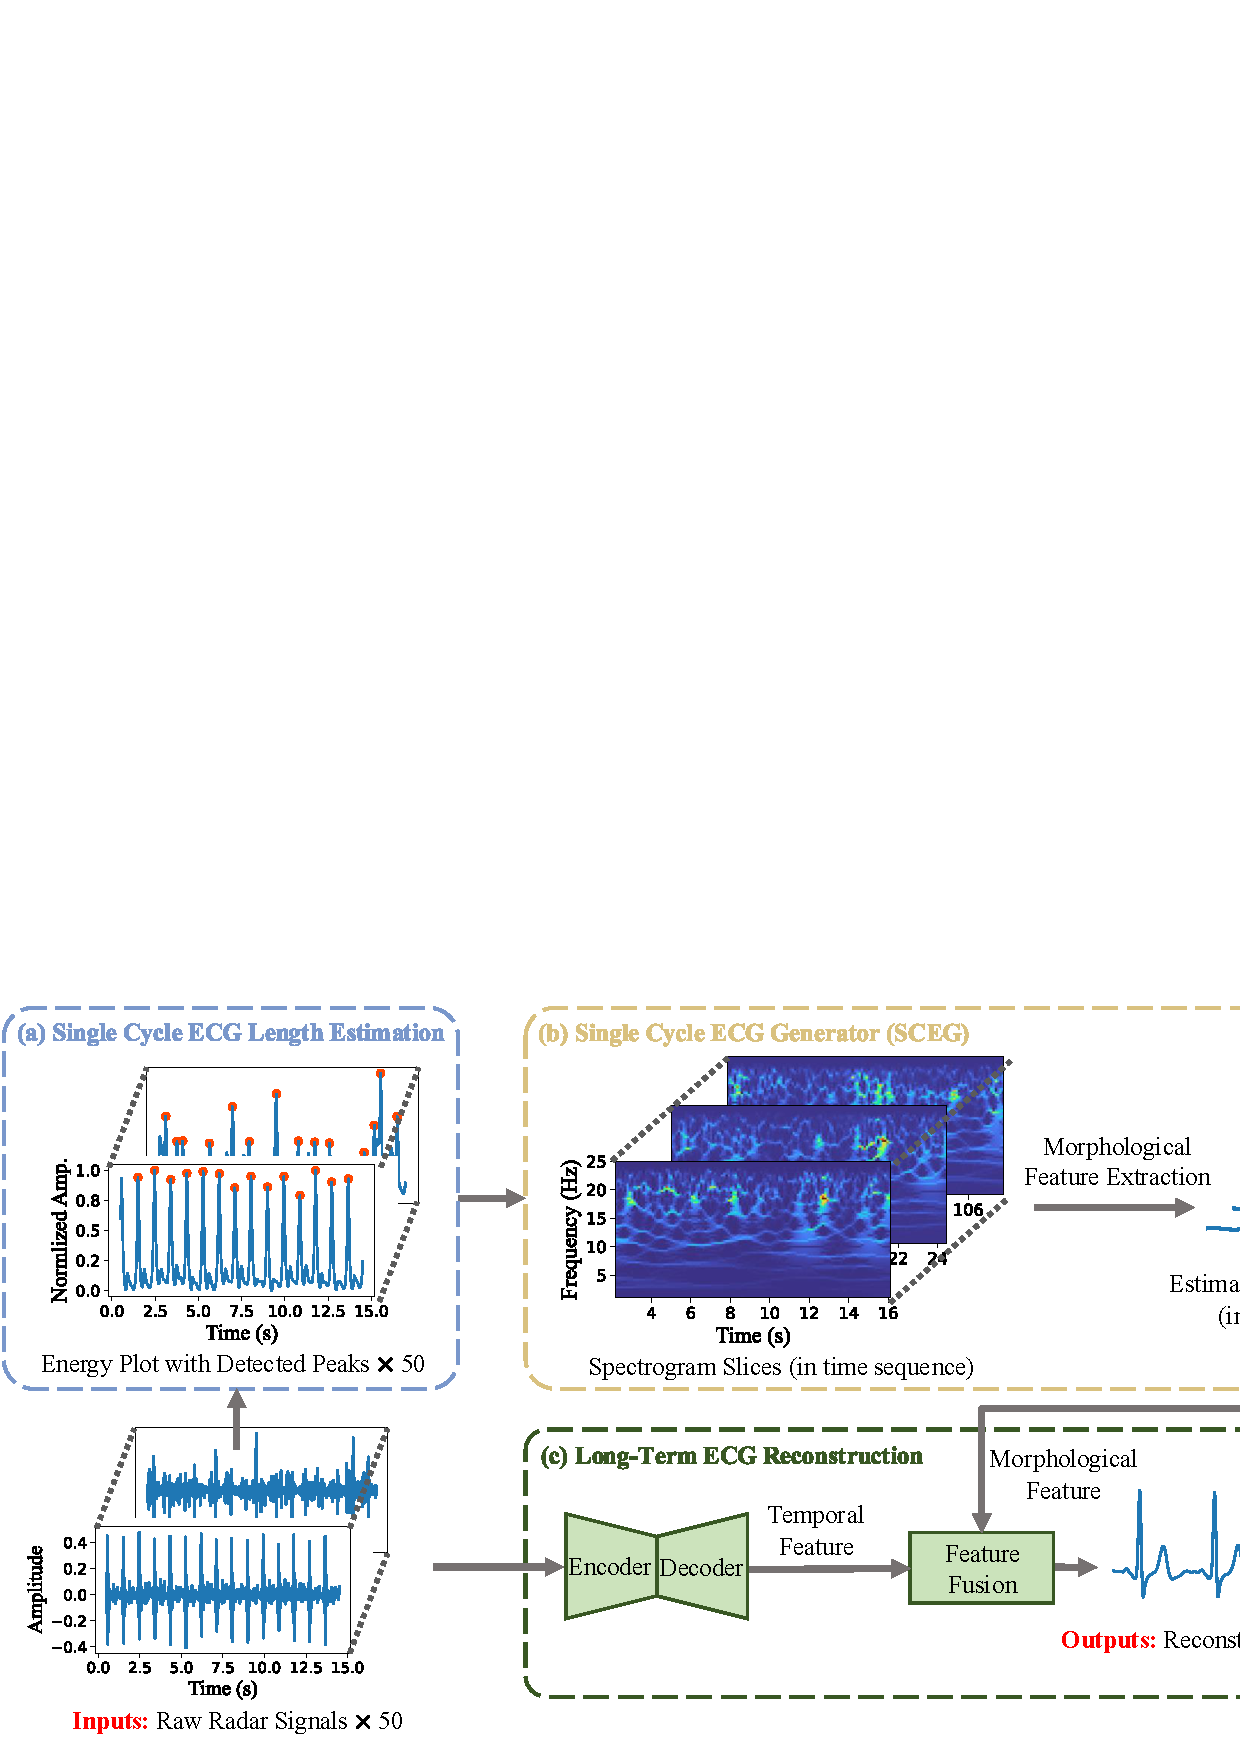
\includegraphics[width=0.99\columnwidth]{main_process.pdf}
    \caption{Overview of the radarODE framework for domain transformation: (a) Single-cycle ECG length (PPI) estimation; (b) Single-cycle ECG generator; (c) Long-term ECG reconstruction.}
    \label{fig:radarODE} 
\end{figure*}
In order to realize a robust radar-to-ECG reconstruction, the proposed radarODE framework is designed based on the domain transformation within a single cardiac cycle to generate faithful ECG reference that aids the domain transformation in long-term ECG recovery. The inputs of radarODE are $50$ synchronous radar signals that represent the measurements from $50$ spatial points within the chest region~\cite{chen2022contactless}, as shown in Figure~\ref{fig:radarODE}, and the entire domain transformation is realized by three modules:

\begin{itemize}
    \item The first module estimates the \gls{ppi} for consecutive heartbeats based on the proposed peak detection algorithm and provides information for single cardiac cycle segmentation, as shown in Figure~\ref{fig:radarODE}(a).
    \item The second module first transforms the time-domain radar signal within a single cardiac cycle into a spectrogram using \gls{sst}. Then, the temporal and ODE decoder within SCEG will generate the faithful ECG pieces as morphological references while resisting noise disruption, as shown in Figure~\ref{fig:radarODE}(b).
    \item The third module is used to fuse the extracted morphological and temporal features hidden in the original radar signal to generate the final ECG recovery, as shown in Figure~\ref{fig:radarODE}(c).
\end{itemize}
  
\subsection{Model for Radar Signal and Pre-Processing}
\subsubsection{Fine-Grained Model for Radar Signal}
According to the literature in Chapter~\ref{ch:LR}, the chest displacement $x(t)$ can be further decomposed as
\begin{equation}
x(t) = x_c(t) + x_r(t) + x_n(t)
\end{equation}
where $x_c(t)$ means cardiac mechanical activities, $x_r(t)$ is respiration induced displacement and $x_n(t)$ is noise term. After the pre-processing, the respiration term has been filtered out, and the actual radar signal $\tilde{x}(t)$ provided in the dataset~\cite{chen2022contactless} can be expressed as 
\begin{equation}
\tilde{x}(t) = x_c(t) + x_n(t)
\end{equation}

Furthermore, the pre-processed radar signal $\tilde{x}(t)$ has two prominent vibrations $v_1$ and $v_2$ as shown in Figure~\ref{fig:scg_ecg}, corresponding to the fine-grained cardiac mechanical activities shown in SCG. According to the previous work on SCG modeling, the heart muscle contraction has a pulsatile nature, and the bones/tissues in chest area introduce the extra damping into the pulse~\cite{nosrati2018accurate}. Inspired by the natural characteristics, the radar signal with two prominent vibrations measured in a single cardiac cycle is innovatively modeled as the Gaussian pulses with certain central frequencies as
\begin{equation}\label{equ:vib}
\tilde{x}(t) = v_1(t) + v_2(t) + x_n(t)
\end{equation}
with
\begin{equation}
\begin{aligned}
 v_1 &= \mathrm{a}_1 \mathrm{cos}(2\pi f_1 t)\exp \left(-\frac{(t-T_1)^2}{{b_1}^2}\right)\\
v_2 &= \mathrm{a}_2 \mathrm{cos}(2\pi f_2 t) \exp \left(-\frac{(t-T_2)^2}{{b_1}^2}\right)
 \end{aligned}
\end{equation}
where $a_1$, $b_1$ and $a_2$, $b_2$ jointly contribute to the amplitudes and length of the first and second prominent vibrations, $f_1$, $f_2$ are the corresponding central frequencies, $T_1$, $T_2$ determine when the vibrations happen, and $x_{n}(t)$ represents all the noises. 

The aim of proposing the model in (\ref{equ:vib}) is not to perform the curve fitting but to provide the explanation for the later radarODE design, because the positions of the prominent vibrations ($T_1$, $T_2$) are crucial to the precise reconstruction of ECG peaks using deep neural network.

\subsubsection{Signal Pre-Processing with Synchrosqueezed Wavelet Transform (SST)}
Based on the proposed radar signal model in (\ref{equ:vib}), the next step is to enhance the prominent vibrations (i.e., $T_1$, $T_2$). Figure~\ref{fig:scg_ecg} shows that the high SNR radar signal could reveal prominent peaks of $v_1$ and $v_2$ in the time domain, but in most cases, these two peaks (especially $v_2$) could be ruined by noise. Therefore, this research decides to extract the time-frequency domain information from the spectrogram obtained by synchrosqueezed wavelet transform (SST)~\cite{daubechies2011synchrosqueezed}, and the two vibrations can then be localized by the SCEG module proposed later in Section~\ref{sec:sceg}. 

SST evolves from \gls{cwt} but with concentrated energy distribution along the frequency axis, providing a sparser time-frequency representation with enhanced prominent vibrations compared with other tools such as \gls{stft} and CWT.

The first step of SST is to calculate the CWT of radar signal $\tilde{x}(t)$ as
\begin{equation}
W_{\tilde{x}}(a, b)=\int \tilde{x}(t) a^{-1 / 2} \psi^*\left(\frac{t-b}{a}\right) d t
\end{equation}
where $\psi^*$ is the complex conjugate of the chosen mother wavelet, and $a$, $b$ are the adjustable scaling and translation factors for the wavelet $\psi$ to extract frequency- and time-domain information, respectively. In this research, the Morlet wavelet is selected as mother wavelet because it is widely used for vibration signal processing, especially for time-frequency localization~\cite{xue2023novel}.

The second step is to calculate the candidate instantaneous frequency for $W_{\tilde{x}}(a, b)\neq 0$ as
\begin{equation}
f_{\tilde{x}}(a, b)=-2\pi i\left(W_{\tilde{x}}(a, b)\right)^{-1} \frac{\partial W_{\tilde{x}}(a, b)}{\partial b}
\end{equation}

The final step is to concentrate the energy along the candidate instantaneous frequency as
\begin{equation}
T_{\tilde{x}}(2\pi f, b)=\int_{A(b)} W_{\tilde{x}}(a, b) a^{-3 / 2} \delta\left(2\pi f_{\tilde{x}}(a, b)-2\pi f\right) d f
\end{equation}
where $A(b)=\left\{a ; W_{\tilde{x}}(a, b) \neq 0\right\}$, and $\delta$ represents the Dirac-delta function in a distribution version to smoothly squeeze the spread-out energy into a narrow band around the instantaneous frequency~\cite{daubechies2011synchrosqueezed}.

The quality of the resultant spectrograms can be evaluated using \gls{pse}~\cite{wang2023vital}, with a small value indicating that the energy is concentrated around a certain frequency. The calculated PSE for the spectrogram produced by STFT, CWT and SST is $0.94$, $0.90$ and $0.76$ respectively, with the visualized results shown in Figure~\subref*{fig:compare_stft},~\subref*{fig:compare_cwt} and~\subref*{fig:compare_sst}. It is clear that the spectrogram obtained by STFT only shows the rough positions of each $v_1$, while CWT gives a sharp position for both vibrations, but the energy is still spread out. By further concentrating the energy distribution, SST produces the spectrogram with a relatively clean background and sharp peaks for the vibrations, reducing the burden of the deep-learning-based SCEG module in extracting latent features (i.e., $T_1$, $T_2$).

\begin{figure}[tb]
        \centering
        \subfloat[]{\label{fig:compare_radar}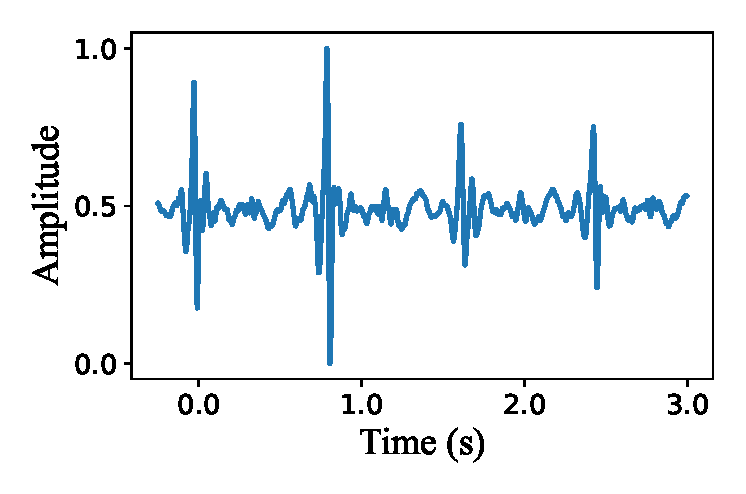
\includegraphics[width=0.4\columnwidth]{compare_radar.eps}}
        \subfloat[]{\label{fig:compare_stft}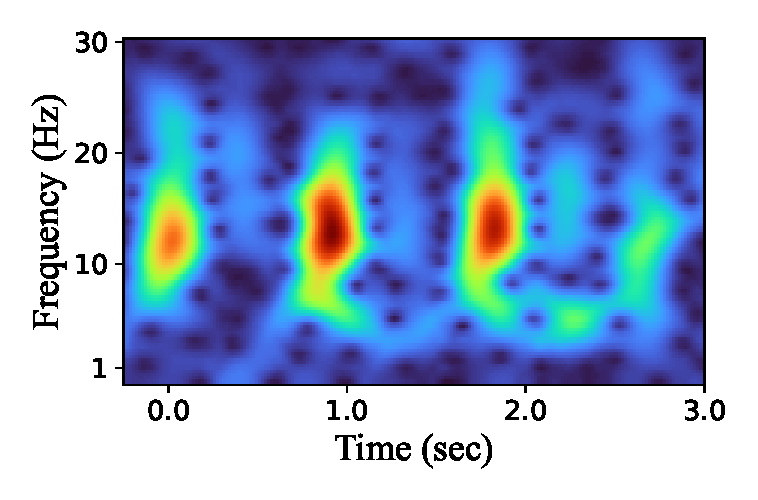
\includegraphics[width=0.4\columnwidth]{compare_stft.eps}} \\ \vspace{-0.01\columnwidth}
        \subfloat[]{\label{fig:compare_cwt}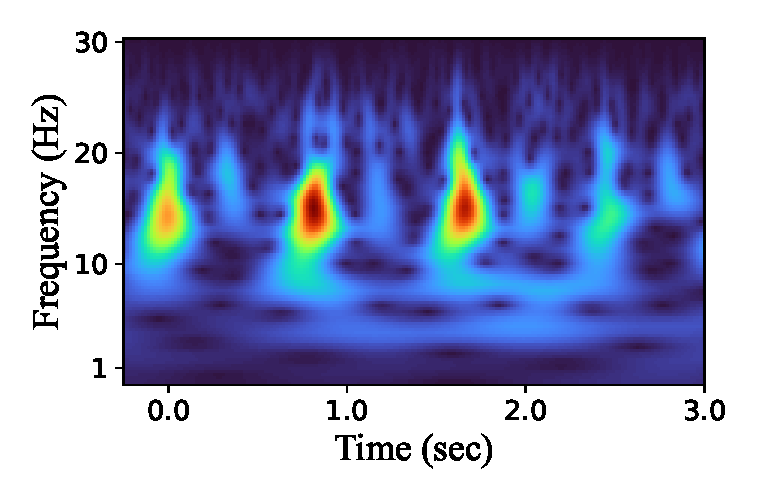
\includegraphics[width=0.4\columnwidth]{compare_cwt.eps}}
        \subfloat[]{\label{fig:compare_sst}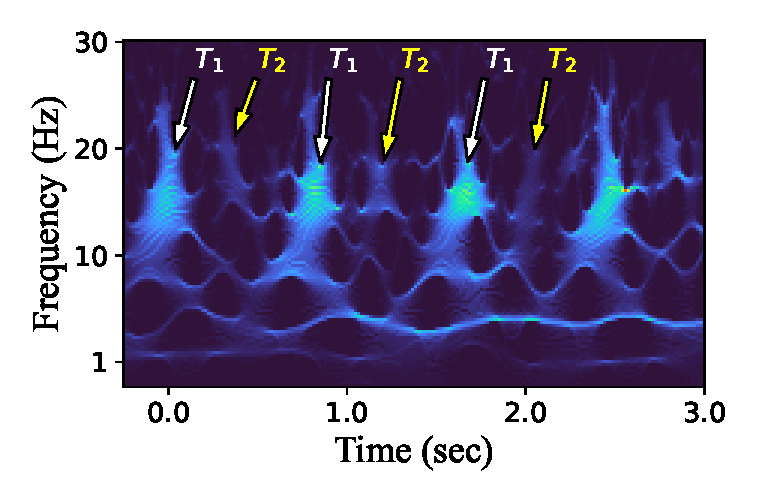
\includegraphics[width=0.4\columnwidth]{compare_sst.eps}} 
        \caption{Spectrograms obtained from the same radar signal: (a) Radar signal $\tilde{x}(t)$; (b) STFT result; (c) CWT result; (d) SST result with $T_1$, $T_2$ labeled, revealing concentrated energy around vibrations and clean background.}
        \label{fig:spec_compare}
\end{figure}

\subsection{radarODE Framework Design}
\subsubsection{Single-cycle ECG Length Estimation}
The first module of radarODE aims to estimate the length of each single-cycle ECG piece by calculating the interval between two consecutive heartbeats (i.e., PPI) from the energy plots $\hat{x}$ of the radar signal $\tilde{x}$ (omit $(t)$ for simplicity) as shown in Figure~\subref*{fig:correct_detection}. The energy plot is obtained by simply adding the spectrogram along frequency axis, but the peak detection results may not be promising due to low SNR signals as shown in Figure~\subref*{fig:wrong_detection}. Therefore, a new algorithm is proposed as in Algorithm~\ref{alg:ppi} to eliminate the wrong detection obtained from $50$ radar energy plots ${X}_{\mathcal{L}}$, with the length of each $\hat{x}_{i}\in {X}_{\mathcal{L}}$ equal to $l$.

The design of Algorithm~\ref{alg:ppi} is based on the fact that the PPI for healthy people tends to be unchanged in adjacent cardiac cycles. In this case, the long-term radar energy plots are firstly sliced into short segments as shown in the \textsc{Initialization} stage in Algorithm~\ref{alg:ppi}, and then the biopeaks algorithm implemented in NeuroKit2~\cite{makowski2021neurokit2} is used for detecting all the potential peaks $P$ from each energy plot segment $\hat{x}^j_i$ as:
\begin{equation}\label{equ:biopeak}
P = biopeaks(\hat{x}^j_i)
\end{equation}
Secondly, the resultant $PPI_\mathcal{C}$ obtained from Line~\ref{line:biopeaks}-\ref{line:update} in Algorithm~\ref{alg:ppi} contains potential estimated PPI from $50$ radar energy plots, with the correct estimations as the majority. Therefore, the \gls{kde}~\cite{terrell1992variable} is applied on the candidate set $PPI_\mathcal{C}$ to calculate the probability density of different PPI values as:
\begin{equation}\label{equ:kde}
KDE:\ \hat{f}(p)=\frac{1}{n h} \sum_{c=1}^n K\left(\frac{p-PPI_{c\in \mathcal{C}}}{h}\right)
\end{equation}
where $\hat{f}(p)$ means the estimated probability density function at point $p$, $n$ is the number of all the estimated PPI in $PPI_\mathcal{C}$, $K$ is the Gaussian kernel function and $h=n^{-1 /5}$ is the bandwidth of the kernel. Lastly, the final PPI for the current segment is selected as the argument $p$ when $\hat{f}(p)$ achieves the maximum as in Line~\ref{line:final} in Algorithm~\ref{alg:ppi}, and the long-term PPI estimation can be obtained step by step as Algorithm~\ref{alg:ppi} terminated.
\begin{figure}[tb]
        \centering
        \subfloat[]{\label{fig:correct_detection}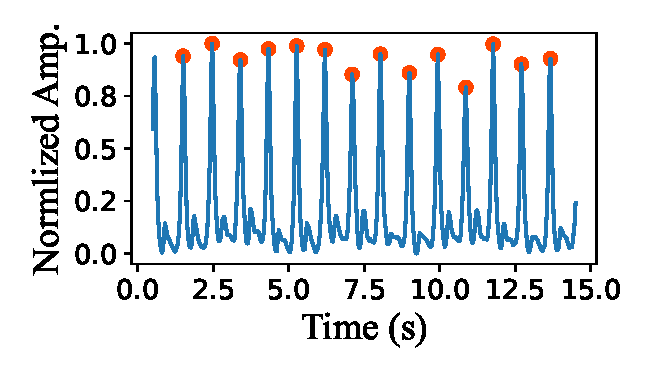
\includegraphics[width=0.4\columnwidth]{correct_detection.eps}}
        \subfloat[]{\label{fig:wrong_detection}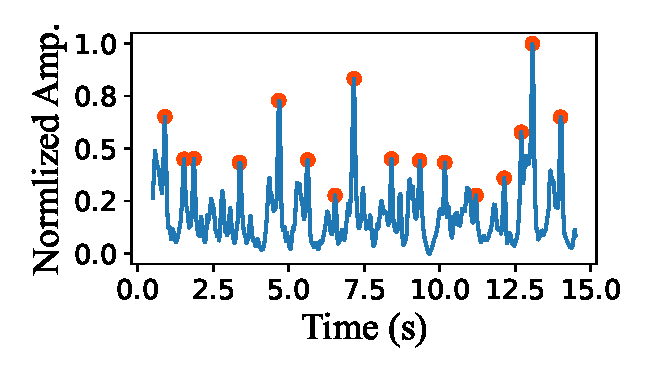
\includegraphics[width=0.4\columnwidth]{wrong_detection.eps}}
        \caption{Energy plot of the synchronous radar signals with different detected peaks: (a) Energy plot with high SNR and correct detection; (b) Energy plot with low SNR and wrong detection.}
        \label{fig:detection_compare}
\end{figure}

\begin{algorithm}[tb]
\caption{PPI Estimation}\label{alg:ppi}
\begin{algorithmic}[1]
    \State \textbf{Input:} \multiline{0.9}{Radar Energy Plots ${X}_{\mathcal{L}} = \{\hat{x}_{1},\hat{x}_{2},\ldots,\hat{x}_{50}\}$, Segments Length $l_{seg}$ and \\ Step Length $l_{step}$}
    \State \textbf{Output:} Estimated $PPI$
    \Statex \textsc{Initialization}:
    \State\quad - \multiline{0.9}{Let ${X}_{\mathcal{S}}=\{{X}^1_{\mathcal{L}}, {X}^2_{\mathcal{L}},\ldots, {X}^{J}_{\mathcal{L}}\}$ be an ordered list of the segment lists sliced from ${X}_{\mathcal{L}}$ with length $l_{seg}$ and step $l_{step}$, where $J = \frac{l-l_{seg}}{l_{step}}$.}
    \State\quad - Let $PPI \leftarrow \emptyset$.
    \Statex \textsc{Main iteration}:
    \For{each segment list ${X}^j_{\mathcal{L}}\in {X}_{\mathcal{S}}$}
        \State - \multiline{0.9}{Let $PPI_{\mathcal{C}} \leftarrow \emptyset$ to save the candidate PPI obtained from each segment.}
        \For{each segment $\hat{x}^{j}_{i} \in {X}^j_{\mathcal{L}}$}
            \State 1) \multiline{0.9}{ Apply biopeaks~\cite{makowski2021neurokit2} on $\hat{x}^{j}_{i}$ to get all the detected peaks $P$ as in (\ref{equ:biopeak}).} \label{line:biopeaks}
            \State 2) \multiline{0.9}{Get PPI for the current radar signal segment using differentiation as \\ $PPI_c \leftarrow diff(P$).}
            \State 3)  Update $PPI_{\mathcal{C}} \leftarrow PPI_{\mathcal{C}} \cup PPI_c$. \label{line:update}
        \EndFor
    \State - \multiline{0.9}{Calculate the probability density function $\hat{f}(p)$ for $PPI_{\mathcal{C}}$ using KDE as in (\ref{equ:kde}).}
    \State - \multiline{0.9}{Determine the final PPI for the current segment list and update the set as $PPI \leftarrow PPI \cup\arg \max_{p} \hat{f}(p)$.} \label{line:final}
    \EndFor
\end{algorithmic} 
\end{algorithm} 

\subsubsection{Single-cycle ECG Generator (SCEG)}\label{sec:sceg}
Based on the yielded $PPI$, the SST spectrogram can be sliced into segments corresponding to a single cardiac cycle, and the aim of the SCEG module is to reconstruct the ECG for each single cardiac cycle, hence realizing the transformation from mechanical to electrical domain. In general, the input of the SCEG is $N$ segments of the SST plot within $[1,25]$~Hz with the size of $F\times T$ on frequency and time axis, and the output is the corresponding $N$ ECG pieces with the same length $T$, as shown in Figure~\ref{fig:sceg}. In practice, the deep neural network only accepts the inputs/outputs of the same size. Therefore, the actual SST segment is centered at the current cardiac cycle and expands to $4$ seconds, and the corresponding ECG ground truth is resampled to a fixed length of $200$ for loss calculation.

For architecture design, the SCEG module adopts the popular backbone-encoder-decoder structure as verified by enormous image-related tasks~\cite{li2023euclidean,chu2024vessel}, with detailed parameters shown in Table~\ref{tab:param}. In addition, a feature fusion block is added after the decoder to fuse the temporal and morphological features and generate the final ECG reconstructions. The detailed implementation of each part in Table~\ref{tab:param} with explanations can be elaborated as:

\begin{figure*}[tb] 
    \centering 
    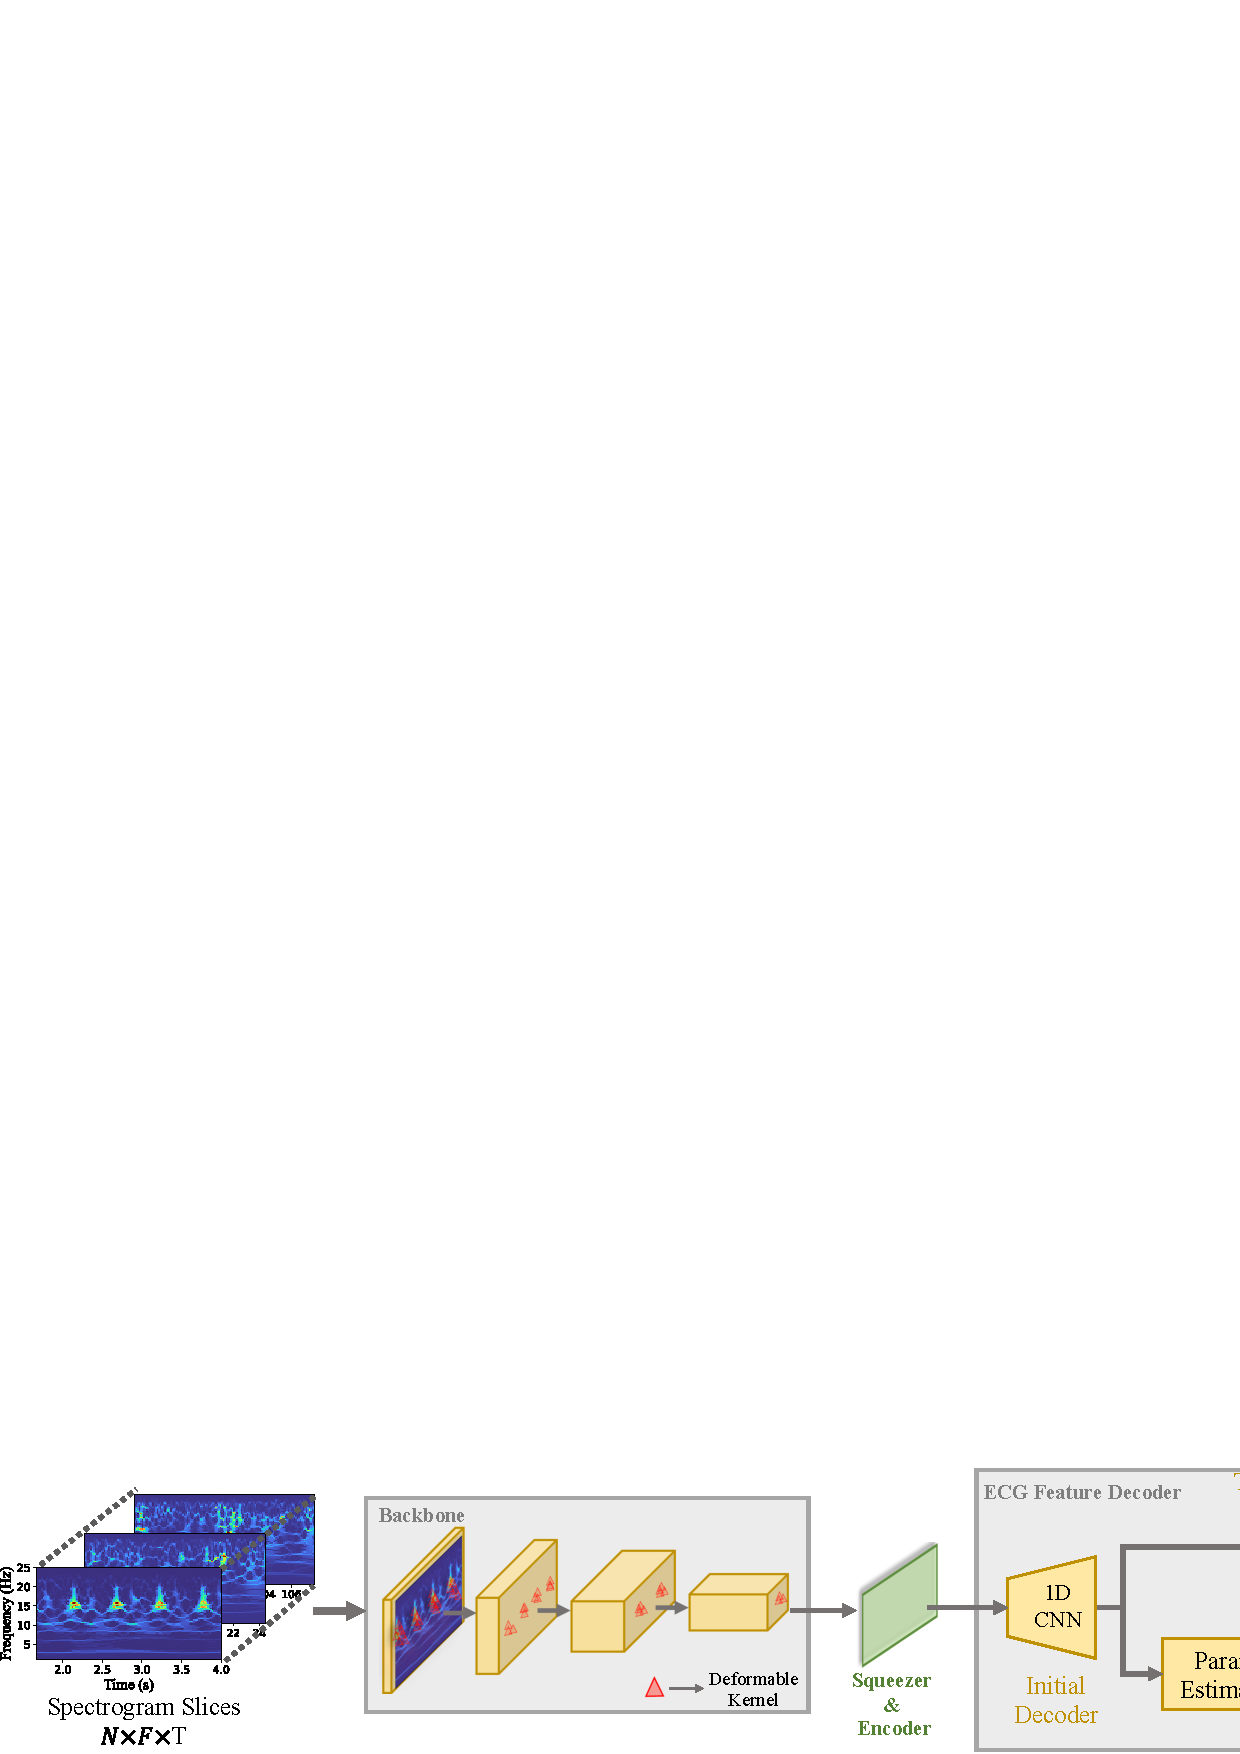
\includegraphics[width=0.8\columnwidth]{SCEG.pdf}
    \caption{Architecture of SCEG with SST segments as input and single-cycle ECG pieces as output.} 
    \label{fig:sceg} 
\end{figure*}

\begin{longtable}{l l l}
\caption{Structure and parameters for SCEG} \label{tab:param} \\

\toprule
\textbf{Layers} & \textbf{Parameters}  & \textbf{Output Shape} \\
& ($C_{in}$, $C_{out}$, $K$, $S$)$^1$ & $N$: Batch Size \\
\toprule
\endfirsthead

\multicolumn{3}{c}%
{{\bfseries \tablename\ \thetable{} -- continued from previous page}} \\
\toprule
\textbf{Layers} & \textbf{Parameters}  & \textbf{Output Shape} \\
& ($C_{in}$, $C_{out}$, $K$, $S$)$^1$ & $N$: Batch Size \\
\toprule
\endhead

\midrule \multicolumn{3}{r}{{Continued on next page}} \\
\endfoot

\bottomrule
\multicolumn{3}{l}{1. $C_{in}$: Input channel,  $C_{out}$: Output channel, $K$: Kernel size, $S$: Stride}\\
\endlastfoot

Input SST &  & $(N, 50, 71, 118)$ \\
\toprule
\textbf{a. Backbone} & & \\
\ \ Residual Block   & $(50,128,(2,1),(1,1))$  & $(N, 128, 72, 118)$\\
\ \ Downsample Block & $(128,128,(3,2),(2,2))$ &  $(N, 128, 36, 60)$\\
\ \ Residual Block   & $(128,256,(2,1),(1,1))$ & $(N, 256, 37, 60)$\\
\ \ Downsample Block & $(256,256,(3,2),(2,2))$ &  $(N, 256, 19, 31)$\\
\ \ Residual Block   & $(256,512,(2,1),(1,1))$ & $(N, 512, 20, 31)$\\
\ \ Downsample Block & $(512,512,(3,3),(2,1))$ &  $(N, 512, 10, 31)$\\
\ \ Residual Block   & $(512,1024,(2,1),(1,1))$ & $(N, 1024, 11, 31)$\\
\ \ Downsample Block & $(1024,1024,(3,3),(2,1))$ &  $(N, 1024, 6, 31)$\\
\toprule
\textbf{b. Squeezer\&Encoder} & & \\
\ \ Conv2d & $(1024,1024,(6,1),(1,1))$  & $(N, 1024, 31)$\\
\ \ Transconv1d Block & $(1024,512,5,3)$ & $(N, 512,95)$ \\
\ \ Transconv1d Block & $(512,256,5,3)$ & $(N, 256,287)$ \\
\ \ Transconv1d Block & $(512,128,5,3)$ & $(N, 128, 863)$ \\
\toprule
\multicolumn{3}{l}{\textbf{c. ECG Feature Decoder}} \\
\multicolumn{3}{l}{\ \ \textbf{Initial Decoder}} \\
\ \ Conv1d Block  & $(128,64,7,2)$ & $(N,64,430)$ \\
\ \ Conv1d Block  & $(64,32,7,2)$ & $(N,32,213)$ \\
\ \ Conv1d Block  & $(32,16,7,1)$ & $(N,16,209)$ \\
\ \ Conv1d Block  & $(16,8,5,1)$ & $(N,8,207)$ \\
\multicolumn{3}{l}{\ \ \textbf{Temporal Feature Decoder}} \\
\ \ Conv1d  & $(8,4,7,1)$ & $(N,4,203)$ \\
\ \ Conv1d  & $(4,2,5,1)$ & $(N,2,201)$ \\
\ \ Conv1d  & $(2,1,2,1)$ & $(N,1,200)$ \\
\ \ \textbf{ODE Decoder} & \\
\ \ Linear Block & $(8*207, 512,-,-)$ & $(N, 512)$  \\
\ \ Linear Block & $(512, 128,-,-)$ & $(N, 128)$  \\
\ \ Linear Block & $(128, 32,-,-)$ & $(N, 32)$ \\
\ \ Linear Block & $(32, 16,-,-)$ & $(N, 16)$  \\
\ \ ODE Solver   & $-$ & $(N,1,200)$ \\
\toprule
\textbf{d. Feature Fusion} & &  \\
\ \ Feature Multiply  &  $-$ & $(N,1,200)$ \\
\ \ Stack  &  $-$ & $(N,1,4,200)$ \\
\ \ Conv2d Block  & $(1,16,(5,5),(1,2))$ & $(N,16,2,98)$ \\
\ \ Conv2d Block  & $(16,32,(3,3),(1,2))$ & $(N,32,2,48)$ \\
\ \ Conv2d Block  & $(32,64,(3,3),(2,2))$ & $(N,64,1,23)$ \\
\ \ Transconv1d Block  & $(64,32,5,2)$ & $(N,32,52)$ \\
\ \ Transconv1d Block  & $(32,16,5,2)$ & $(N,16,106)$ \\
\ \ Transconv1d Block  & $(16,8,3,2)$ & $(N,8,10,211)$ \\
\ \ Transconv1d  & $(8,4,6,1)$ & $(N,4,206)$ \\
\ \ Transconv1d  & $(4,2,5,1)$ & $(N,2,202)$ \\
\ \ Transconv1d  & $(2,1,3,1)$ & $(N,1,200)$ \\
\bottomrule
\multicolumn{2}{l}{Output single-cycle ECG piece} &  $(N, 1, 200)$ \\
\end{longtable}
\begin{enumerate}[a.]
\item \textbf{Backbone: } Backbone is typically used as the first block to extract both low-level (e.g., color, edge) and high-level features (e.g., presence of specific pattern) from the input images. In the context of this research, the backbone is expected to localize the vibrations $v_1$, $v_2$ revealed as periodically appeared bright triangles within the range of $[1,25]~Hz$ on SST plots, providing latent information of $T_1$, $T_2$ for the further ECG reconstruction. 

\quad According to the literature, ResNet with residual blocks is widely used as the backbone for feature extraction in many fields~\cite{chen2024tfpred}, and this research will use a similar structure with $4$ layers of residual blocks and downsample blocks as shown in Figure~\ref{fig:backbone}, with the key parameters listed in Table~\ref{tab:param}. In addition, the traditional 2D convolution is all replaced by deformable 2D convolution~\cite{dai2017deformable} with deformable kernels (instead of square kernels) to fit the irregular shape of the target patterns, as shown in red triangles in Figure~\ref{fig:sceg}.
\begin{figure}[tb] 
    \centering 
    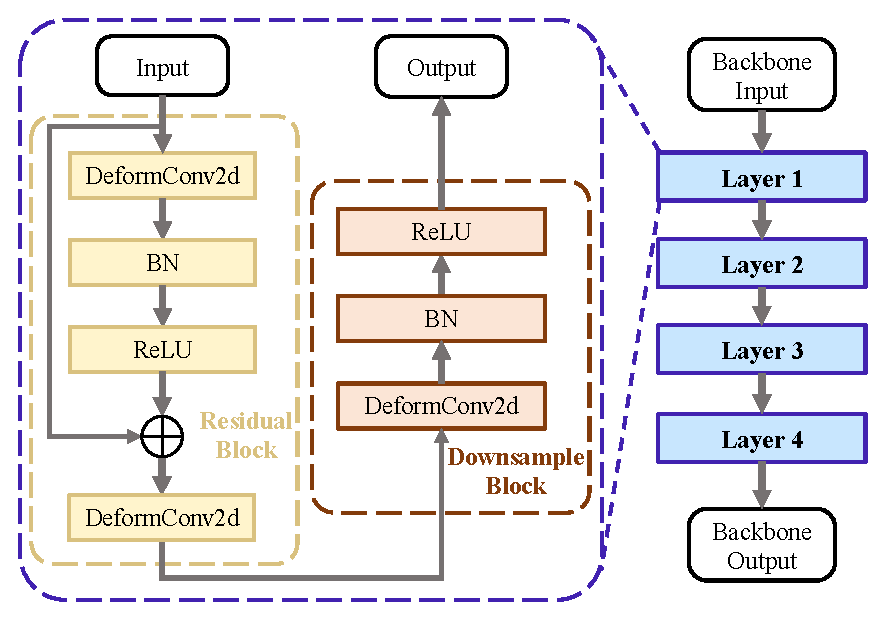
\includegraphics[width=0.7\columnwidth]{backbone.eps}
    \caption{Structure of backbone composed of residual block and downsample block: DeformConv2d means deformable 2D convolution, BN is batch normalization, and ReLU is the rectified linear unit activation function.} 
    \label{fig:backbone} 
\end{figure}

\item \textbf{Squeezer and Encoder: } The output feature map from the backbone should involve both frequency- and time-domain features, and the squeezer is simply used to squeeze the frequency-domain feature using 2D convolution (Conv2d) and output the feature map with the temporal feature only. Then, the encoder assembled by three 1D transposed convolution (Transconv1d) blocks is used to further extract the temporal feature, with each block comprising Transconv1d, BN and ReLU. Finally, the output feature map from the encoder should contain latent information about $v_1$, $v_2$ (i.e., ($T_1$, $T_2$)).

\item \textbf{ECG Feature Decoder: }The decoder is an essential part of SCEG to extract the temporal and morphological features separately from the latent information in the SST feature map, as shown in two branches in Figure~\ref{fig:sceg}. At first, an initial decoder is shared by the latter two decoders and comprises four 1D convolution (Conv1d) blocks with Conv1d, BN, and ReLU inside. Similarly, the temporal feature decoder is assembled by three Conv1d, and the output feature should contain prominent peaks at the position of $T_1$, $T_2$. However, these two peaks may still have deviations from the peaks in ECG ground truth, because obviously the mechanical vibrations $v_1$, $v_2$ lag behind QRS-complex and T-peaks, as shown in Figure~\ref{fig:scg_ecg}. Another problem with the temporal feature decoder is that the ECG pieces have an entirely different shape with radar measurements, and the decoder needs to `memorize' the unique pattern of ECG. Although the previous work shows the deep neural network could learn the patterns after training, the whole process of ECG reconstruction lacks supervision and is vulnerable to noise in radar signals~\cite{chen2022contactless,yang2022pipeline}.

\begin{table}[tb]
\centering
\caption{Default values for $\eta$}
    \begin{tabular}{cccccc}
    \toprule
    \diagbox{$\mathbf{\eta}$}{$\mathbf{\mathcal{F}}$} & $\mathbf{e_P}$ &  $\mathbf{e_Q}$& $\mathbf{e_R}$ & $\mathbf{e_S}$ & $\mathbf{e_T}$\\
    \toprule
    $a_{e_f}$ & $5$ & $-100$ & $480$ & $-120$ & $8$ \\
    $b_{e_f}$ & $0.25$ & $0.1$ & $0.1$ & $0.1$ & $0.4$ \\
    $\theta_{e_f}$ & $\frac{-15\pi}{180}$ & $\frac{25\pi}{180}$ & $\frac{40\pi}{180}$ & $\frac{60\pi}{180}$ & $\frac{135\pi}{180}$ \\
    \bottomrule
    \end{tabular}%
\label{tab:ode_value}%
\end{table}%

In this case, the ODE decoder is designed as a branch to assist the transformation between cardiac mechanical and electrical activities. The main obstacles in modeling such domain transformation are the lack of (a) A compact model for ECG signal and (b) A corresponding explanation between parameters in describing radar signal and ECG signal, e.g., what is the relationship between R peak and $v_1$ in Figure~\ref{fig:scg_ecg}. In this work, the aforementioned two obstacles can be solved from the following perspectives:
\begin{itemize}
    \item The shape of the ECG piece can be modeled morphologically using ODEs in a compact form without any biological/chemical knowledge~\cite{mcsharry2003dynamical}.
    \item The measurements of mechanical activities generally lag behind those of electrical activities with a short time delay $\tau$~\cite{swift2021stop,orkand1964heart}.
\end{itemize}

\quad Inspired by the above facts, the ODE decoder is designed as a parameter estimation part and an ODE solver as shown in Figure~\ref{fig:sceg}, and the solution of the ODEs will be shifted to the left with time $\tau$. In this manner, the latent information in describing radar signals is first transformed to the parameters for the ECG signal, and then the ODE solver will generate morphological-prior to accelerate the convergence of the model training process and provide extra robustness against noises.

\quad To be specific, the parameters estimation part contains four linear blocks (Linear Layer, BN, Tanh) to project the latent space yielded by the initial decoder into parameters $\eta$, $\tau$, and $\eta$ will be sent to an ODE solver to solve a 3D trajectory denoted by $(x,\ y,\ z)$ as
\begin{equation}\label{equ:ode}
    \left\{
    \begin{aligned}
    & \frac{d x}{d t}=\alpha(x, y) x-\omega y \\
    & \frac{d y}{d t}=\alpha(x, y) y+\omega x \\
    & \frac{d z}{d t}=-\sum_{e_f\in \mathcal{F}} a_{e_f} \Delta \theta_{e_f}(x, y) e^{-\Delta \theta_{e_f}(x, y)^2 / 2 b_{e_f}^2}-z
    \end{aligned}
    \right. 
\end{equation}
    with
    \begin{equation}
    \begin{aligned}
    \alpha(x, y) & =1-\sqrt{x^2+y^2} \\
    \Delta \theta_{e_f}(x, y) & =\left(\theta(x, y)-\theta_{e_f}\right) \quad \bmod 2 \pi \\
    \theta(x, y) & =\operatorname{atan} 2(y, x)) \in[-\pi, \pi] \\
    e_f\in\mathcal{F} & =\{e_P, e_Q, e_R, e_S, e_T\}
    \end{aligned}
\end{equation}
where $\mathcal{F}$ represents five characteristic peaks (PQRST) in a single-cycle ECG signal, and the whole ODEs can be interpreted as manipulating each peak along a unit circle by varying the value of $\eta=\{a_{e_f},b_{e_f},\theta_{e_f}\}$ to adjust corresponding amplitude, width and position of each peak. After specifying all $15$ parameters $\eta$ ($3$ for each peak) and the initial conditions of $(x,y,z)$, the value of $z$ can be solved by the ODE solver using the Euler method to get the final single-cycle ECG signal as the morphological feature. In practice, the default values for $\eta$ are provided in advance as in Table~\ref{tab:ode_value}, and the estimated parameters within the range of $[-1,1]$ are used to scale the default values.

\item \textbf{Feature Fusion: } The feature fusion module could leverage respective advantages of the morphological and temporal features and generate the final ECG signal for loss calculation, because the morphological feature only focuses on five peaks to provide a rough shape of ECG with calibrated peaks, and the temporal feature reserves all the other feature neglected in (\ref{equ:ode}) to help the final reconstruction~\cite{guan2023achelous}. Therefore, two features are first fused together by multiplication (Mul.) into one and then stacked four times by itself. Then, the stacked feature is encoded and decoded as in Table~\ref{tab:param} to produce the final single-cycle ECG piece.
\end{enumerate}

The last step of SCEG is to resample all the ECG pieces generated after the feature fusion part with respect to the previous PPI estimation, and the resampled ECG pieces are concatenated in a time sequence to form the final morphological reference for long-term ECG reconstruction.

\begin{table}[tb]
\centering
\caption{Structure and parameters for long-term ECG reconstruction}
    \begin{tabular}{l l l}
    \toprule
    \textbf{Layers} & \textbf{Parameters}  & \textbf{Output Shape} \\
    & ($C_{in}$, $C_{out}$, $K$, $S$)$^1$ & $N$: Batch Size \\
    \toprule
    Input raw radar Signal &  & $(N, 50, 800)$ \\
    \toprule
    \textbf{a. Encoder} & & \\
    \ \ Residual Block   & $(50,128,5,1)$  & $(N, 128, 800)$\\
    \ \ Downsample Block & $(128,128,5,2)$ &  $(N, 128, 400)$\\
    \ \ Residual Block   & $(128,256,5,1)$ & $(N, 256, 400)$\\
    \ \ Downsample Block & $(256,256,5,2)$ &  $(N, 256, 200)$\\
    \ \ Residual Block   & $(256,512,5,1)$ & $(N, 512, 200)$\\
    \ \ Downsample Block & $(512,512,5,2)$ &  $(N, 512, 100)$\\
    \toprule
    \textbf{b. Decoder} & & \\
    \ \ Transconv1d Block & $(512,128,5,2)$ & $(N, 128,200)$ \\
    \ \ Transconv1d Block & $(128,16,5,2)$ & $(N, 16,400)$ \\
    \ \ Transconv1d Block & $(16,1,5,2)$ & $(N, 1, 800)$ \\
    \toprule
    \multicolumn{2}{l}{\textbf{c. Feature Fusion (TCN)}}  \\
    \ \ Feature Stack$^2$  &  $-$ & $(N,2,800)$ \\
    \ \ Dilated Conv1d $\times 9$  & $K=3$, $D = 2$ & $(N, 1, 800)$ \\
    \bottomrule
    \multicolumn{2}{l}{Output long-term ECG} &  $(N, 1, 800)$ \\
    \bottomrule
    \multicolumn{3}{l}{1. $C_{in}$: Input channel,  $C_{out}$: Output channel, $K$: Kernel size, $S$: Stride}\\
    \multicolumn{3}{l}{2. Stack with the morphological feature as in Figure~\ref{fig:radarODE}(c).}\\
    \end{tabular}%
\label{tab:long_structure}
\end{table}%

\begin{figure}[tb] 
    \centering 
    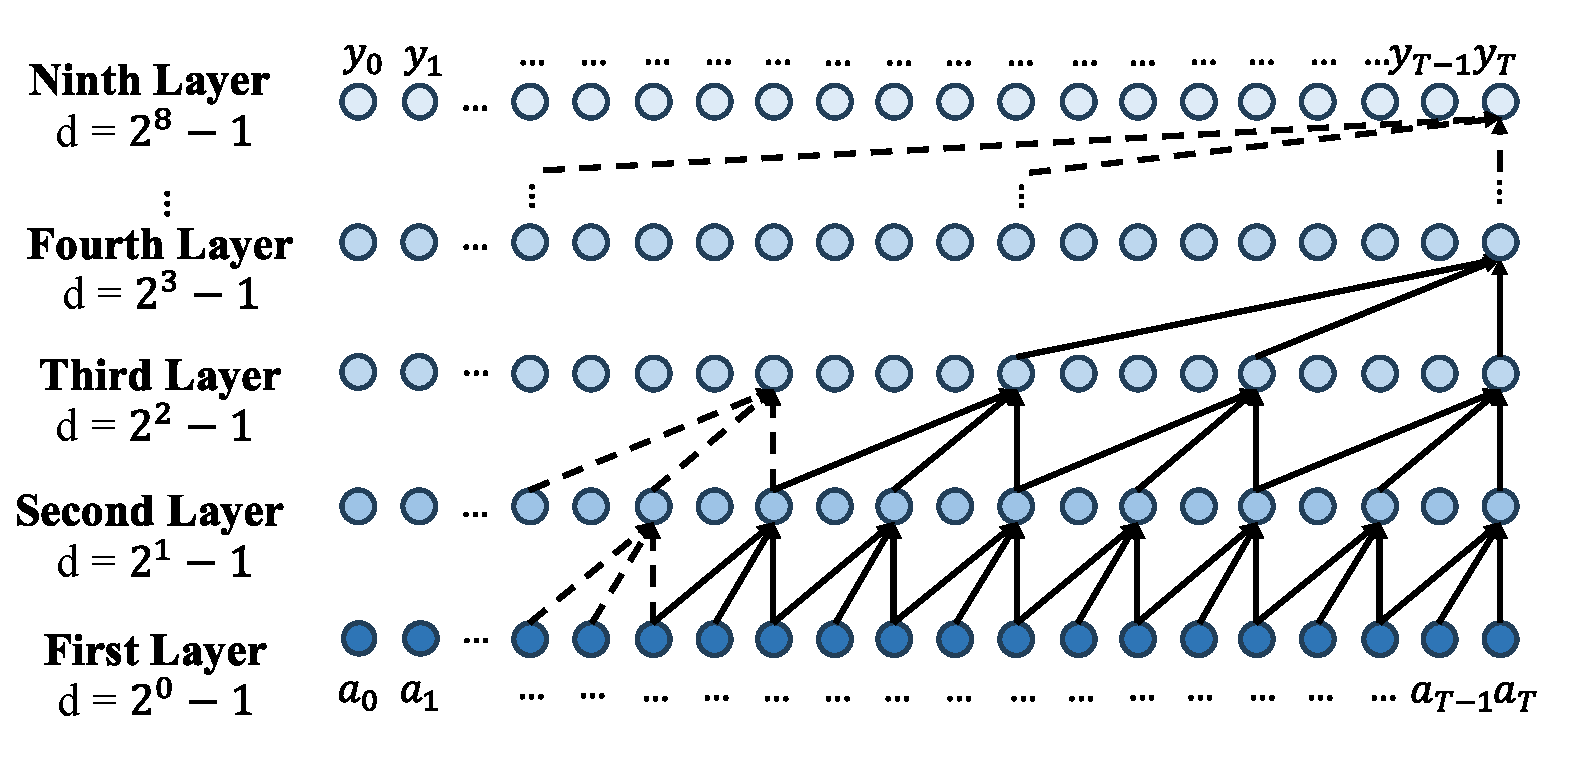
\includegraphics[width=0.9\columnwidth]{TCN.eps}
    \caption{The structure of the $9$-layer TCN with dilation factor $D=2$ and kernel size $K=3$.}
    \label{fig:tcn_net} 
\end{figure}
\subsubsection{Long-Term ECG Reconstruction}
The long-term ECG reconstruction network adopts a similar encoder-decoder-fusion structure with SCEG as shown in Figure~\ref{fig:radarODE}(c), with the detailed structure and parameters shown in Table~\ref{tab:long_structure} and Figure~\ref{fig:tcn_net}. The encoder takes $50$ series of 4-sec time-domain radar signals as input and is composed of three groups of residual and downsample blocks with the deformable 2D convolution in Figure~\ref{fig:backbone} replaced by 1D convolution. Then, the decoder is realized by three Transconv1d blocks to generate the temporal feature.

The temporal feature generated from decoder in Table~\ref{tab:long_structure} will be stacked with morphological feature as illustrated in Figure~\ref{fig:radarODE}(c), and these two features act as two channels for later feature fusion by the \gls{tcn}. In general, TCN adopts dilation 1D convolution (Dilated Conv1d) to process multi-channel data structure using expanded receptive field with gaps between elements as shown in Figure~\ref{fig:tcn_net}, and the feature fusion is achieved during channel reduction as a common technique in traditional convolution neural network~\cite{xue2023novel}. Specifically, the solid line in Figure~\ref{fig:tcn_net} shows the connection of a $4$-layer TCN with the gaps for each layer $l$ as $d=D^{l-1}-1$, and the output $y_T$ is predicted based on a receptive field of $15$ input feature points $\{a_{T-14},\dots,a_T\}$. In this chapter, $9$-layer Dilated Conv1d is adopted with dilation factor $D=2$ and kernel size $K=3$, and the receptive field is $511$ to make the most of contextual information contained in the temporal and morphological features.

\section{Dataset and Implementation Details}\label{sec:odedataset}
\subsection{Hardware and Environment Settings for Data Collection}
The public dataset can be requested from~\cite{chen2022contactless} and is collected by the TI AWR-1843 radar with $77$~GHz start frequency and $3.8$~GHz bandwidth, providing good SNR and resolution to detect subtle vibrations that fit the proposed signal model and framework. To realize the 3D beamforming to extract cardiac features from real 3D space, $3$ transmitters (Tx) and $4$ receivers (Rx) are enabled with \gls{tdmmimo} applied in chirp transmitting and receiving.

The data collection is performed for subjects lying on the bed with quasi-static status to ensure good SNR with the least RBM noise. In addition, radar is placed right above the human chest region in a range of $0.4-0.5$m with minor propagation attenuation as shown in Figure~\ref{fig:env_set}, and hence the large- or small-scale signal variations (e.g., path loss, multi-path fading) are not considered in~\cite{chen2022contactless}.

\begin{figure}[tb] 
    \centering 
    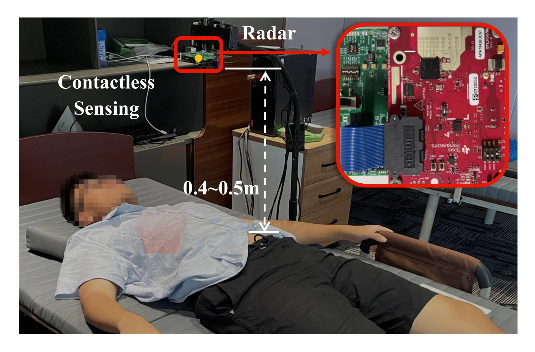
\includegraphics[width=0.6\columnwidth]{env_set.eps}
    \caption{Environment settings for data collection from quasi-static subject~\cite{chen2022contactless}.}
    \label{fig:env_set} 
\end{figure}

\subsection{Link Budget Analysis}
Link budget analysis is a common evaluation for the performance of a radar system by accounting for all gains and losses from the transmitter to the receiver~\cite{mercuri2019vital,lin2022broadband}, but such analysis is not provided in~\cite{chen2022contactless}. For a radar system, the received power $P_{\mathrm{R}}$ can be expressed with respect to the transmitted power $P_{\mathrm{T}}$ as:
\begin{equation}\label{equ:proga}
P_{\mathrm{R}}=\frac{G_{\mathrm{T}} G_{\mathrm{R}} \lambda^2 \sigma}{(4 \pi)^3 R^4} P_{\mathrm{T}}
\end{equation}
where $G_T$/$G_R$ is the gain of the transmitter/receiver, $\sigma$ is the effective radar cross section (RCS) for the human chest region, and $R$ is the distance between radar and chest~\cite{mercuri2019vital}.

In addition, the lowest detectable signal power of the receiver is defined in~\cite{lin2022broadband} as:
\begin{equation}\label{equ:p_desire}
P_{\mathrm{r}, \min}= -174\ \mathrm{dBm} + 10\log_{10}(B) + \mathrm{NF} + \mathrm{SNR}_{\min}
\end{equation}
where $-174$ represents the thermal-noise level, NF means the noise figure, $B$ is the bandwidth of the receiver and $\mathrm{SNR}_{\min}$ is the desired SNR considering the afterward signal processing.

By combining (\ref{equ:proga}) and (\ref{equ:p_desire}), the maximum detectable range can be calculated as:
\begin{equation}\label{equ:r_max}
R_{\text {max}}=\sqrt[4]{\frac{G_{\mathrm{T}} G_{\mathrm{R}} \lambda^2 \sigma P_{\mathrm{T}}}{(4 \pi)^3 \ P_{\mathrm{r}, \min}}}
\end{equation}

All the radar-related values in (\ref{equ:r_max}) are shown in Table~\ref{tab:link_param} according to the datasheet of TI AWR-1843 radar~\cite{AWR1843}. According to the previous work~\cite{lin2022broadband,chen2022contactless}, the RCS value can be estimated as $-20$ dBsm for the quasi-static subjects wearing electrically thin cloth (i.e., the thickness is much smaller than the wavelength), with respiration noise filtered during the pre-processing stage. After substituting the values, the lowest detectable signal power is $P_{\mathrm{r}, \min}=-53$ dBm, and the maximum detectable range is $R_{\text {max}}=4$ m, revealing that the parameter setting used in~\cite{chen2022contactless} could provide the received signal with good SNR.

\begin{table}[tb]
\centering
\caption{Parameters for link budget analysis}
    \begin{tabular}{lc?lc}
    \toprule
    \textbf{Parameter} & \textbf{Value} & \textbf{Parameter} & \textbf{Value} \\
    \toprule
    Tx Gain ($G_T$) & $10$ dBi  & Rx Gain ($G_R$) & $30$ dBi  \\
    Tx power ($P_{\mathrm{T}}$)& $12$ dBm & Noise Figure (NF)     & $15$ dB   \\ 
    Wavelength ($\lambda$)  & $3.9$ mm               & Bandwidth (B)         & $3.8$ GHz \\
    RCS ($\sigma$)     & $-20$ dBsm  &  Desired SNR ($\mathrm{SNR}_{\min}$) & $10$ dB  \\
    \bottomrule
    \end{tabular}%
\label{tab:link_param}
\end{table}%

\subsection{Dataset Description}
Half of the actual dataset is released with $91$ trials for $11$ subjects (with subject ID 1, 2, 5, 9, 10, 13, 14, 16, 17, 29, 30), and each trial contains $3$ minutes of data (radar measurements and ECG ground truth) with $200$~Hz sampling rate collected under $4$ physiological statuses (i.e., normal breath (NB, $43$ trials), irregular breath (IB, $18$ trials), sleep (SP, $18$ trials) and post exercise (PE, $12$ trials)). In addition, the work in~\cite{chen2022contactless} has pre-processed the radar signal using several techniques, such as 3D beamforming, dynamic time wrapping, to remove respiration noise and enhance cardiac activities. Lastly, no existing study is found for ECG reconstruction in literature based on the same dataset, and the proposed framework MMECG in~\cite{chen2022contactless} will be used as the only benchmark to make a comparison with our radarODE.

\subsection{Implementation Details and Compared Frameworks}
The proposed radarODE network is coded using PyTorch and trained for $200$ epochs with batch size $32$ on the NVIDIA RTX A4000 ($16$~GB) using stochastic gradient descent optimizer with early stop function~\cite{yao2007early} and learning rate $0.001$ based on a cosine annealing schedule~\cite{loshchilov2016sgdr}. The dataset is split into training and testing sets based on $11$-fold cross-validation with $1$ fixed subject for testing and the other $10$ subjects alternatively selected for training or validation, ensuring to make the most of all the trials while excluding the testing data from the training phase. In addition, all the ground truth characteristic peaks, PPI, and cardiac cycles are obtained by the NeuroKit2 from ECG signals~\cite{makowski2021neurokit2}. Furthermore, the $4$-seconds-long input SST segments only contain the frequency component within $[1,25]$~Hz and are down-sampled to $30$~Hz in the time-axis for saving memory usage in backbone design. 

In addition, three frameworks are selected for comparison with the following brief introduction of the architecture:
\begin{itemize}
  \item MMECG~\cite{chen2022contactless} receives multiple 1D radar signals as input and utilizes Conv1d and Transformer as decoder to simultaneously extract temporal and spatial features. The encoded features are further fused by multiplication and then decoded by Transconv1d and TCN to produce ECG recovery. 
  \item RSSRNet~\cite{wu2023contactless} takes spectrogram (STFT) as input with a Conv2d backbone and Transformer encoder. The adopted decoder is Transconv2d, and the output is still a spectrogram and needs to be converted to the ECG signal via inverse STFT.
  \item RadarNet~\cite{li2024radarnet} adopts 1D radar signal as input and directly generates coarse ECG signal using Conv1d. Then, several layers of ResNet are adopted to refine the ECG waveform.
\end{itemize}

\section{Experimental Results and Evaluations}\label{sec:odeexp}
This section provides the experimental results and evaluations in terms of three core modules as depicted in Figure~\ref{fig:radarODE}, with the first module providing PPI estimation for input/output slicing and reshaping, the second module robustly generating ECG pieces for the single cardiac cycle, and the third module yielding the final long-term ECG recovery.

\subsection{Evaluations of PPI Estimation} \label{sec:ppi}
The PPI estimation is the first module of radarODE, and the accuracy of the estimated PPI directly affects the fidelity of the concatenated morphological reference. Therefore, Figure~\subref*{fig:ppi_obj} shows the PPI estimation error obtained by Algorithm~\ref{alg:ppi} for all subjects based on KDE defined in (\ref{equ:kde}) or directly averaging the candidate PPI values. The large PPI error (e.g., for subject $13$, $17$) is normally caused by body movements or residual respiration noise due to IB or PE status, as also shown in Figure~\subref*{fig:ppi_phy} with large median error and variation for both methods. In contrast, the subjects in NB and SP statuses tend to be stable with less body movement, and the respiration noise can be well eliminated, achieving low median PPI errors as $0.03$s and $0.02$s using the KDE-based method for each status.

Overall, it is clear that the KDE-based PPI estimation is more accurate than the mean-based estimation for each subject, as shown in the \gls{cdf} in Figure~\subref*{fig:ppi_cdf}, because the KDE-based method is robust to the outliers caused by noises and could figure out the correct PPI estimation near the majority of candidate values.
\begin{figure}[tb]
        \centering
        \subfloat[]{\label{fig:ppi_obj}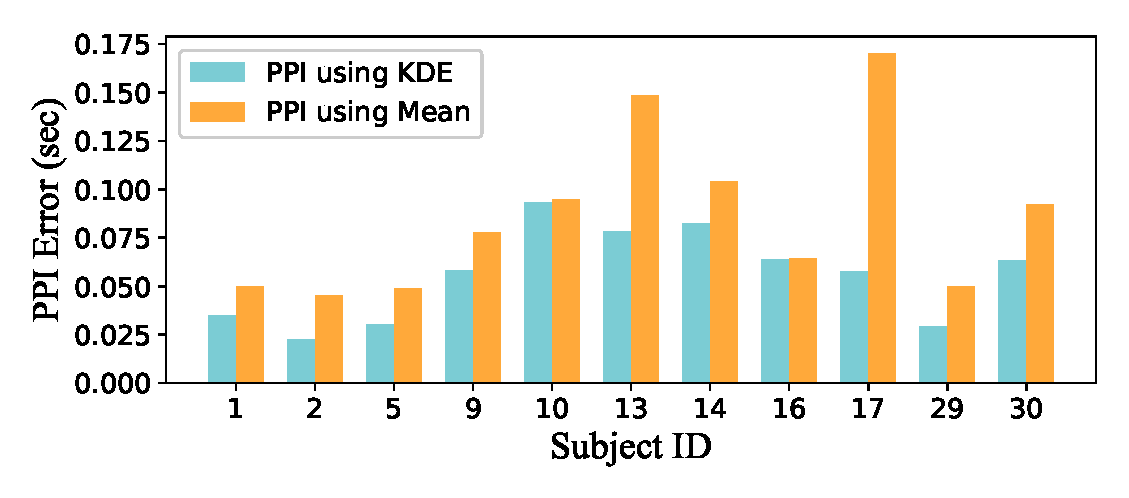
\includegraphics[width=0.7\columnwidth]{ppi_obj.eps}}\\ \vspace{-0\columnwidth}
        \subfloat[]{\label{fig:ppi_phy}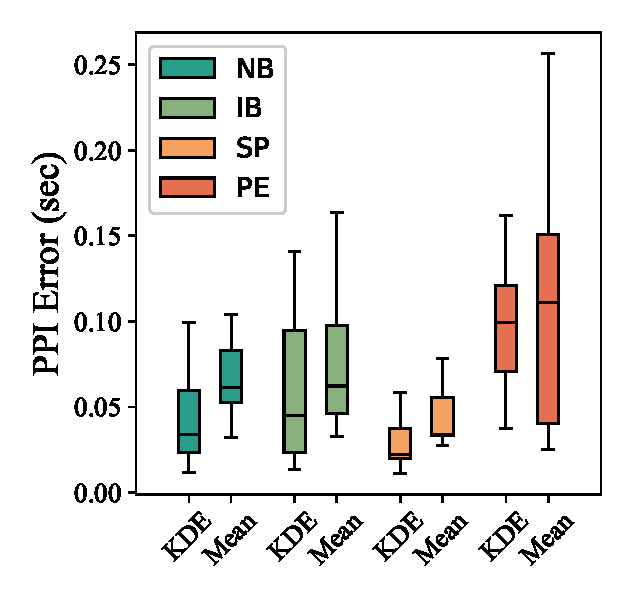
\includegraphics[width=0.35\columnwidth]{ppi_phy.eps}}
        \subfloat[]{\label{fig:ppi_cdf}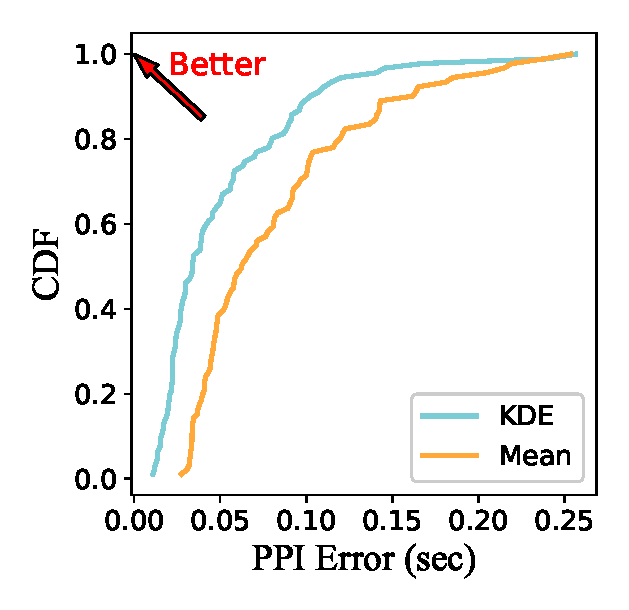
\includegraphics[width=0.34\columnwidth]{ppi_cdf.eps}}
        \caption{PPI estimation error of KDE-based and mean-based method: (a) View of different subjects; (b) View of different physiological statuses; (c) CDF for the overall PPI estimation error.}
        \label{fig:ppi_compare}
\end{figure}

\begin{figure}[tb]
  \centering
  \subfloat[]{\label{fig:rmse_cdf_compare}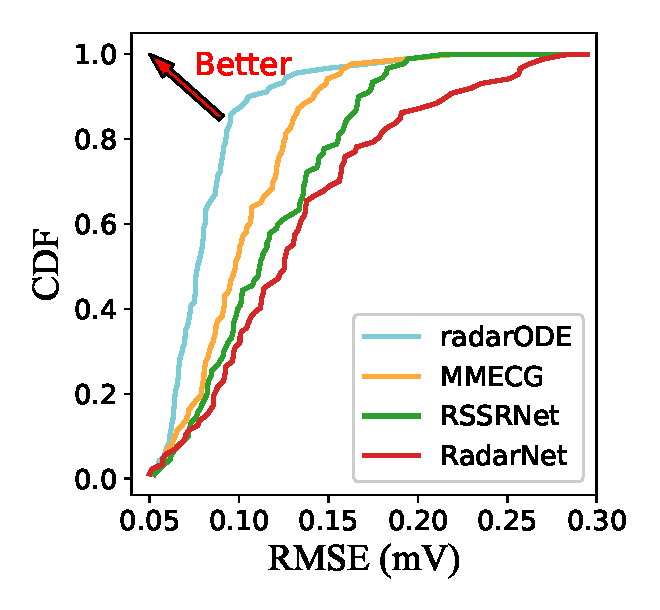
\includegraphics[width=0.35\columnwidth]{rmse_cdf_compare.eps}}
  \subfloat[]{\label{fig:sceg_cor_cdf}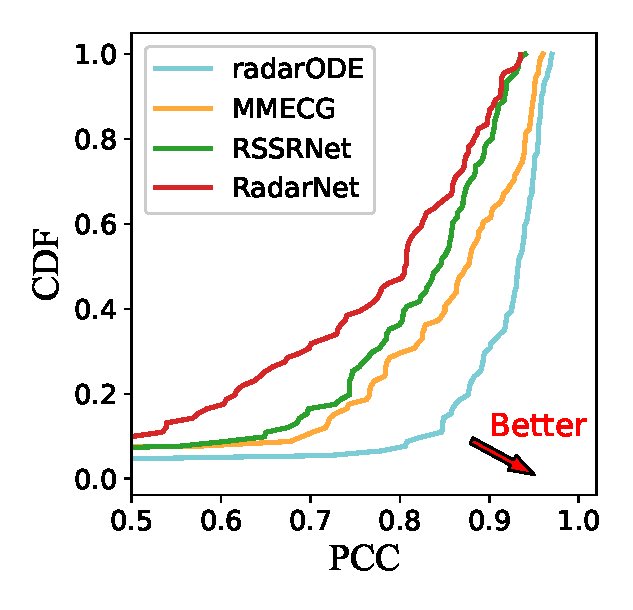
\includegraphics[width=0.33\columnwidth]{sceg_cor_cdf.eps}}\\
  \subfloat[]{\label{fig:MDR_cdf_overall}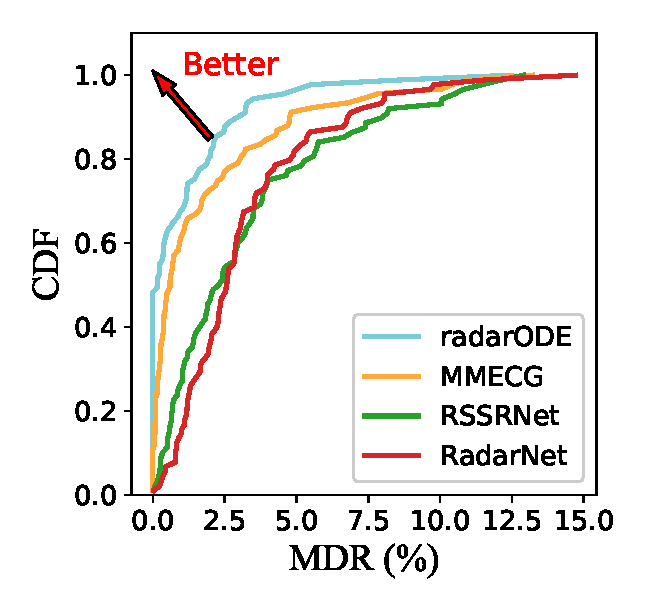
\includegraphics[width=0.34\columnwidth]{MDR_cdf_overall.eps}}
  \subfloat[]{\label{fig:sceg_r_cdf}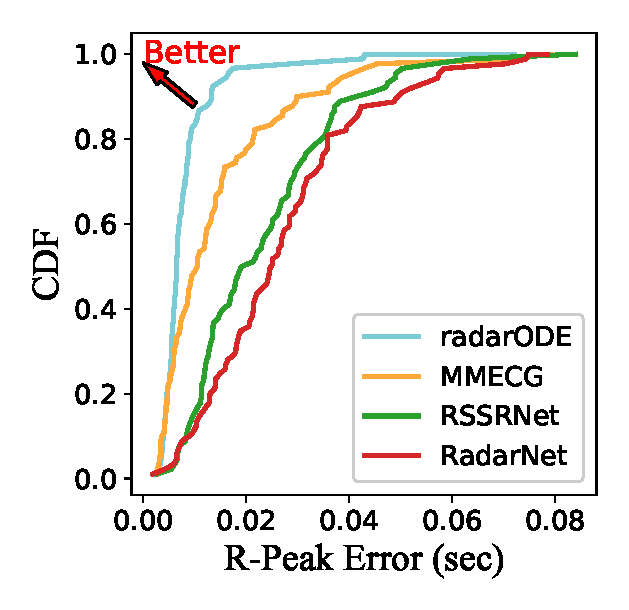
\includegraphics[width=0.33\columnwidth]{sceg_r_cdf.eps}}
  \caption{Performance comparison for single-cycle ECG recovery: (a) - (d) CDF of RMSE, PCC, MDR and R-peak error for all trials.}
  \label{fig:sceg_performance}
\end{figure}
\subsection{Evaluations of SCEG Module in radarODE}
SCEG is the core module that realizes the domain transformation and ensures the robust long-term ECG recovery in the next stage, and the performance is evaluated on the generated single-cycle ECG pieces in terms of morphological accuracy, corrupt ECG reconstruction and absolute R-peak error as shown in Figure~\ref{fig:sceg_performance} and Table~\ref{tab:ablation}.

\subsubsection{Comparison of Morphological Accuracy}
The morphological accuracy is shown in Table~\ref{tab:ablation} as the median value of \gls{rmse} and \gls{pcc}, with RMSE sensitive to the deviation of peaks and PCC focusing on the general shape. The overall performances for all trials are shown as CDF plots in Figure~\subref*{fig:rmse_cdf_compare} and~\subref*{fig:sceg_cor_cdf}. The results indicate that radarODE could generate high-fidelity ECG signals with good RMSE and PCC owing to the prior knowledge provided by the ODE decoder, while MMECG achieves the second-best result and shows a domain transformation ability for the majority of radar inputs with good SNR. In contrast, RSSRNet and RadarNet achieve a similar performance because they only accept single-channel inputs and cannot effectively leverage the features of $50$ channels provided in the dataset.

\subsubsection{Comparison of Corrupt ECG Recovery}
The ability to recover ECG pieces from corrupt radar signals reveals the noise robustness of each framework, and \gls{mdr} is adopted to count failed recoveries without showing characteristic ECG patterns (R peaks). Three rules are made to define the failed ECG recoveries:
\begin{itemize}
\item The deviation of the corrupt R peak from the ground truth exceeds the absolute tolerance of $0.15$s~\cite{chen2022contactless}.
\item The corrupt R peak has one or more neighboring R peaks closer than $0.3$s.
\item The amplitude of the corrupt R peak is $30\%$ lower than that of the ground truth R peak.
\end{itemize}

The results of MDR are shown in Table~\ref{tab:ablation} with CDF plots of all trials shown in Figure~\subref*{fig:MDR_cdf_overall}. It is evident that radarODE achieves better noise robustness compared with previous work, owing to the constraint brought by ODE decoder. MMECG still has a better performance compared with RSSRNet and RadarNet due to the powerful backbone to extract features from undistorted channels. The overall performance of MDR in Figure~\subref*{fig:MDR_cdf_overall} coincides with the morphological accuracy in Figure~\subref*{fig:rmse_cdf_compare} and~\subref*{fig:sceg_cor_cdf}, because the corrupt ECG recoveries also significantly affect the RMSE and PCC.

\subsubsection{Comparison of R-peak Timing Error}
After filtering the corrupt ECG pieces, the absolute timing error of R peaks is calculated to evaluate the quality of fine-grained ECG features, with the median value and CDF plots shown in Table~\ref{tab:ablation} and Figure~\subref*{fig:sceg_r_cdf} respectively. The results are still similar to previous evaluations, with radarODE recovering the most accurate R peaks and the other three frameworks showing larger R-peak deviation. In addition to the benefits brought by ODE decoder, the adopted SST inputs also provide necessary time-frequency features to help the deep learning model identify indistinctive vibrations under low-SNR scenarios.
\begin{table}[tb]
\centering
\caption{Performance comparison for single-cycle ECG recovery and ablation study}
\resizebox{\textwidth}{!}{%
    \begin{tabular}{c c c c | c c c c}
    \toprule
    Framework & Backbone & Encoder & Decoder  & RMSE (mV) & PCC & MDR & R Error (sec)\\
    \toprule
    MMECG~\cite{chen2022contactless} & - & Conv1d + Transformer & Transconv1d + TCN & $0.091$  & $87.9\%$ & $1.24\%$ & $0.012$ \\
    RSSRNet~\cite{wu2023contactless} & Conv2d & Transformer & Transconv2d  & $0.100$ & $86.0\%$ & $2.17\%$ & $0.019$\\
    RadarNet~\cite{li2024radarnet} & - & Conv1d & Conv1d (ResNet) & $0.113$ & $80.2\%$ & $2.58\%$ & $0.024$\\
    \hline
    \multirow{3}*{radarODE}  & \multirow{3}*{\makecell[c]{Deform\\Conv2d}} & \multirow{3}*{Conv1d}  & Initial + Temporal & $0.086$  & $89.4\%$  & $1.53\%$ & $0.012$\\
    & &  & Initial + ODE & $0.092$ & $85.5\%$ & $\mathbf{0.14\%}$ & $\mathbf{0.005}$ \\
    & &  & Initial + Temporal + ODE  & $\mathbf{0.077}$ & $\mathbf{92.6\%}$ & $0.18\%$ & $0.006$\\
    \bottomrule
    \end{tabular}%
}
\label{tab:ablation}
\end{table}

\begin{figure}[tb]
  \centering
  \subfloat[]{\label{fig:ode_sceg}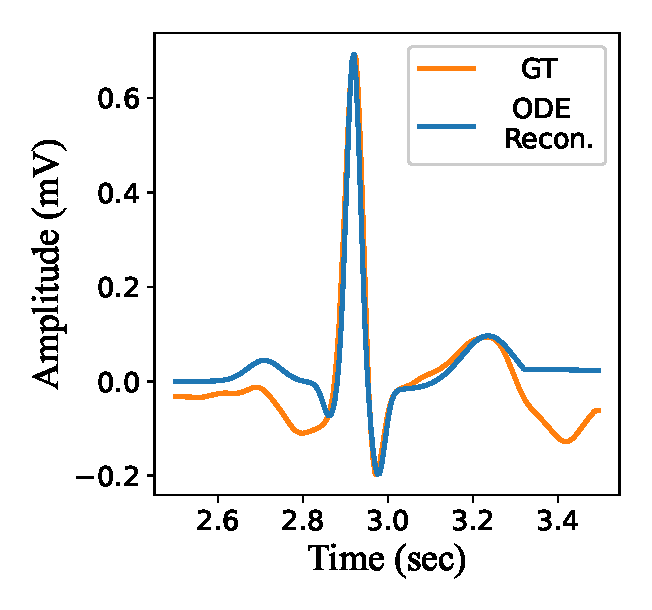
\includegraphics[width=0.4\columnwidth]{ode_sceg.eps}}
  \subfloat[]{\label{fig:loss_compare}\includegraphics[width=0.4\columnwidth]{loss_compare.eps}}
  \caption{Ablation study for training process: (a) Rigid reconstruction (ODE Recon.) from ODE decoder with ground truth (GT); (b) Training loss comparison.}
  \label{fig:sceg_ablation}
\end{figure}

\begin{figure}[tb]
  \centering
  \subfloat[]{\label{fig:sceg_good}\includegraphics[width=0.38\columnwidth]{sceg_good.eps}}
  \subfloat[]{\label{fig:sceg_bad}\includegraphics[width=0.4\columnwidth]{sceg_bad.eps}}
  \caption{Visualization of misalignment: (a) and (b) High- and Low-fidelity morphological references (Ref.) caused by PPI estimation error.}
  \label{fig:sceg_ablation2}
\end{figure}
\subsubsection{Ablation Study} 
The ablation study is performed to further evaluate the contributions of temporal and ODE decoders. The results in Table~\ref{tab:ablation} reveal that both decoders can work individually and achieve reasonable results, but the ODE decoder has lower accuracy because it neglects the subtle ECG feature while only focusing on the characteristic peaks with rigid connections elsewhere, as shown in Figure~\subref*{fig:ode_sceg}. On the contrary, the introduced ODE model could resist strong noise and achieve the lowest MDR as $0.14\%$, while the temporal decoder only gets a similar MDR ($1.53\%$) with MMECG ($1.24\%$). In radarODE, the outputs of temporal and ODE decoder are fused together to achieve noise robustness with MDR$=0.18\%$, while maintaining a faithful ECG shape (i.e., good RMSE and PCC).

\begin{figure}[tb]
    \centering
    \subfloat[]{\label{fig:overall_ode}\includegraphics[width=0.5\columnwidth]{overall_ode.eps}} 
    \subfloat[]{\label{fig:overall_mmecg}\includegraphics[width=0.5\columnwidth]{overall_mmecg.eps}}\\
    \subfloat[]{\label{fig:overall_noise}\includegraphics[width=0.5\columnwidth]{overall_noise.eps}}
    \subfloat[]{\label{fig:overall_rcg}\includegraphics[width=0.5\columnwidth]{overall_rcg.eps}}\\

    \caption{Corrupt ECG reconstruction: (a) and (b) Ideal reconstruction results for radarODE and MMECG; (c) Corrupt ECG reconstruction yield by MMECG and faithful reconstruction from radarODE; (d) Corresponding radar signal during body movements.}
    \label{fig:overall_compare}
\end{figure}

\begin{figure}[tb]
    \centering
    \subfloat[]{\label{fig:detection_cdf_overall}\includegraphics[width=0.3\columnwidth]{detection_cdf_overall.eps}}
    \subfloat[]{\label{fig:detection_cdf_phy}\includegraphics[width=0.3\columnwidth]{detection_cdf_phy.eps}}
    \caption{Statistical results for corrupt ECG reconstruction: (a) Overall missed detection rate (MDR); (b) MDR under different physical statuses.}
    \label{fig:overall_compare_2}
\end{figure}

\subsubsection{Visualization of Training Process} 
Figure~\subref*{fig:loss_compare} illustrates the training loss for benchmark and ablation study with the dotted line representing the early stop of the training process and the shaded area indicating the repetition of the training process for five times. From the ablation study, SCEG with only ODE decoder cannot provide a very accurate reconstruction due to the rigid shape as shown in Figure~\subref*{fig:ode_sceg}, while the temporal decode could achieve the second-best result. After combining ODE and temporal decoders, the outputs from ODE decoder act as the morphological-prior to accelerate the convergence, achieving the RMSE of $0.17$mV after the first epoch. In addition, the morphological reference will not be destroyed by noises and could stabilize the training process, contributing to the lowest training loss as shown in Figure~\subref*{fig:loss_compare}.

\subsubsection{Summary of SCEG Evaluation} 
The proposed SCEG module in radarODE achieves better accuracy in generating single-cycle ECG pieces with the improvements brought by the ODE decoder and SST inputs, enabling successful recoveries even under abrupt noises and achieving the best RMSE, PCC and R-peak accuracy compared with previous frameworks. 

The generated ECG pieces can be resized and concatenated based on PPI estimation, but the PPI estimation error may accumulate and degrade the accuracy as shown in Figure~\subref*{fig:sceg_good} and~\subref*{fig:sceg_bad}, because slight deviations of the peaks ruin the overall RMSE/PCC, hence requiring long-term reconstruction module to refine the concatenated ECG pieces in the next step. To provide a comprehensive evaluation for long-term ECG recovery from various dimensions (e.g., trials, subjects, and physical statuses), MMECG is selected as the only benchmark in the next section for a clear result visualization.

\subsection{Overall Evaluations of radarODE}\label{sec:overall_ode}
The long-term ECG reconstruction module finally generates 3-minute-long ECG signals for the evaluations of the entire radarODE framework in terms of corrupt ECG reconstruction, morphological accuracy, and fine-grained cardiac feature accuracy.

\subsubsection{Corrupt ECG Reconstruction} 
The ideal reconstructed ECG signals are shown in Figure~\subref*{fig:overall_ode} and~\subref*{fig:overall_mmecg} with corresponding RMSE/PCC labeled. However, the long-term ECG signal may contain corrupt parts due to the presence of body movements (especially in IB and PE). Figure~\subref*{fig:overall_noise} shows the corrupted ECG reconstruction yield by MMECG with the falsely detected R peaks noted as red dots, and Figure~\subref*{fig:overall_rcg} is the raw radar signal with extensive distortion induced by body movements. In contrast, the radarODE could still provide faithful ECG reconstructions under body movements due to the introduction of prior knowledge (ODE model) about ECG as the morphological reference, hence gaining certain robustness in resisting noises.
\begin{figure}[tb]
    \centering
    \subfloat[]{\label{fig:rmse_cdf}\includegraphics[width=0.35\columnwidth]{rmse_cdf.eps}}
    \subfloat[]{\label{fig:cor_cdf}\includegraphics[width=0.35\columnwidth]{cor_cdf.eps}}
    \caption{Morphological accuracy comparison for all trials: (a) and (b) Overall CDF of RMSE and PCC for all trials.}
    \label{fig:rmse_cor}
\end{figure}

\begin{figure}[tb]
    \centering
    \subfloat[]{\label{fig:rmse_obj}\includegraphics[width=0.65\columnwidth]{rmse_obj.eps}}\\
    \subfloat[]{\label{fig:cor_obj}\includegraphics[width=0.65\columnwidth]{cor_obj.eps}}
    \caption{Morphological accuracy comparison across all subjects: (a) and (b) RMSE and PCC across all subjects.}
    \label{fig:rmse_cor2}
\end{figure}

\begin{figure}[tb]
    \centering
    \subfloat[]{\label{fig:rmse_phy}\includegraphics[width=0.35\columnwidth]{rmse_phy.eps}}
    \subfloat[]{\label{fig:cor_phy}\includegraphics[width=0.35\columnwidth]{cor_phy.eps}}
    \caption{Morphological accuracy comparison for different physical statuses: (a) and (b) RMSE and PCC under different physical statuses.}
    \label{fig:rmse_cor3}
\end{figure}

The overall MDR can be calculated from the recovered ECG signal with the CDF plot shown in Figure~\subref*{fig:detection_cdf_overall}, and the overall improvement achieved by radarODE is $9\%$. In addition, the CDF plots for different physical statuses are plotted in Figure~\subref*{fig:detection_cdf_phy} with the $90$-percentile MDR of $0.12\%$, $0.85\%$, $0.32\%$, $3.71\%$ during NB, IB, SP, PE for radarODE and $3.36\%$, $6.22\%$, $0.83\%$, $9.64\%$ for MMECG. The result shows that different physical statuses have noticeable impacts on the quality of the reconstructed long-term ECG, and radarODE could provide a lower MDR than MMECG in all statuses owing to the prior knowledge in the ODE decoder.

\subsubsection{Morphological Accuracy}
The morphological accuracy measures the similarity between reconstructed and ground truth ECG signals by calculating RMSE and PCC. Figure~\subref*{fig:rmse_cdf} and~\subref*{fig:cor_cdf} show the overall performance of radarODE and MMECG in CDF with the median RMSE and PCC of $0.097$mV$/89.6\%$ and $0.120$mV$/81.2\%$. It is worth noticing that the overall improvement of radarODE compared to MMECG is $16\%$ and $19\%$ for RMSE and PCC across $91$ trials respectively, indicating that the morphological-prior is more helpful in generalizing the typical ECG pattern than calibrating the peaks.

In addition, Figure~\subref*{fig:rmse_obj} and~\subref*{fig:cor_obj} illustrate the RMSE/PCC across all subjects, with radarODE always achieving better results than MMECG. It is worth noting that the results of the long-term reconstruction show certain consistency with the previous PPI estimation error, because the fidelity of the morphological reference is directly affected by the PPI error. For example, subjects $10$, $13$, $14$, and $30$ get worse results than others in either RMSE or PCC evaluation due to the large PPI estimation error as shown in Figure~\subref*{fig:ppi_obj}.

Lastly, Figure~\subref*{fig:rmse_phy} and~\subref*{fig:cor_phy} illustrate the RMSE/PCC for all trials in terms of different physical statuses, and the box plots show that the stable statuses (i.e., NB, SP) guarantee the reconstruction with small variance. In contrast, unstable statues (i.e., IB, PE) can severely ruin the radar signal due to body movements, causing an inconsistent quality of the reconstructed ECG. However, radarODE could still provide the reconstructions with a smaller variance than MMECG, especially for unstable statues because of the morphological-prior embedded in the ODE decoder.

\begin{figure}[tb]
  \centering
  \includegraphics[width=0.75\columnwidth]{peak_cdf.eps}
  \caption{CDF of the overall timing error.}\label{fig:peak_cdf}
  \label{fig:peak_compare}
\end{figure}

\begin{figure}[tb]
  \centering
  \subfloat[]{\label{fig:peak_phy_ode}\includegraphics[width=0.4\columnwidth]{peak_phy_ode.eps}}
  \subfloat[]{\label{fig:peak_phy_mmecg}\includegraphics[width=0.4\columnwidth]{peak_phy_mmecg.eps}} 
  \caption{Evaluations of fine-grained cardiac events: (a) and (b) The timing error for different peaks under various physical statuses for radarODE and MMECG.}
  \label{fig:peak_compare2}
\end{figure}

\subsubsection{Fine-Grained Cardiac Events Reconstruction}
The evaluation of fine-grained cardiac features aims to analyze the timing accuracy of the QRST peaks and the P peak is not considered in this evaluation as also suggested in~\cite{chen2022contactless}, because the P peak is inconspicuous and even unable to be detected for some ground truth ECG signal. The overall result is shown in Figure~\ref{fig:peak_cdf} as CDF with the median/$90$-percentile absolute timing error for QRST peaks shown in Table~\ref{tab:peak_acc}. The improvement owes to the use of SST spectrogram with more evident patterns for the prominent heart vibrations, and the ODE decoder contributes to calibrating the peak positions according to $\eta$ and $\tau$, hence improving the overall peak accuracy.

\begin{table}[tb]
\centering
\caption{Absolute timing error for reconstructed ECG peaks}
    \begin{tabular}{c c cccc}
    \toprule
    Framework & Percentile & Q & R & S & T \\
    \toprule
    \multirow{2}*{MMECG~\cite{chen2022contactless}} & Median & $0.021$ & $0.012$ & $0.019$ & $0.018$ \\
                                           & $90$-percentile & $0.048$ & $0.023$ & $0.029$ & $0.035$ \\
    \toprule 
    \multirow{2}*{radarODE}                         & Median & $0.015$ & $0.007$ & $0.009$ & $0.014$ \\
                                           & $90$-percentile & $0.027$ & $0.015$ & $0.020$ & $0.023$ \\
    \bottomrule
    \multicolumn{6}{r}{unit: second} \\
    \end{tabular}%
\label{tab:peak_acc}
\end{table}%

Figure~\subref*{fig:peak_phy_ode} and~\subref*{fig:peak_phy_mmecg} demonstrate the improvement of radarODE in terms of different physical statuses, and the results coincide with many previous evaluations. Firstly, the radarODE outperforms MMECG for all statuses with the R peak always achieving the best accuracy. Secondly, stable physical statuses tend to yield accurate reconstruction with small variance, but the difference between statues is smaller than that of the morphological accuracy analysis, because the corrupt reconstructions have been filtered for peak accuracy evaluation. 

\subsubsection{Summary of Long-term ECG Recovery Evaluation} 
The experimental results illustrated that the proposed radarODE could yield high-quality long-term ECG recovery even under extensive body movement noise, with better RMSE and PCC compared with the benchmark. In addition, the introduction of the SST spectrogram and the ODE decoder further improves the accuracy of the fine-grained cardiac features that are crucial to the potential applications in clinical diagnosis.

\section{Conclusions}\label{sec:odeconclusions}
Radar-based ECG reconstruction is highly reliant on purely data-driven approaches and lacks theoretical support regarding the transformation between mechanical activities measured by radar and electrical activities described as ECG. This research aims to bridge the gap to realize the transformation from the mechanical domain to the electrical domain by proposing the signal model with fine-grained features considered and further designing a deep learning framework radarODE with morphological prior embedding as ODEs. The radarODE framework is validated on the public dataset containing $4.5$ hours of radar measurements with corresponding ablation study and comparisons with the benchmark. The experimental result shows that radarODE could achieve a better MDR, morphological accuracy and peak accuracy than the benchmark, proving the rationality of the proposed signal model and the effectiveness of the radarODE under various physical statuses and random body movement.
\chapter{Robust Long-Term ECG Generation}\label{ch:radarMTL}
This chapter further extends the robust single-cycle ECG recovery to the robust long-term ECG recovery by leveraging \gls{mtl} as a popular paradigm to help the concatenation of the well-recovery ECG pieces. According to the experiments in Chapter~\ref{ch:radarODE}, the misalignment cause by inaccurate \gls{ppi} estimation heavily ruin the final results, and it is necessary to design the long-term ECG recovery based on single-cycle ECG pieces, instead of realizing the recovery process in terms of arbitrary divided radar/ECG pairs. Therefore, a novel MTL structure designed for long-term ECG recovery is designed with three sub-tasks responsible for recovering different ECG features. In addition, a optimization strategy is also designed to balance the training process for the sub-tasks with great disparity in terms of intrinsic difficulties. Sufficient experiments show that the proposed radarODE-MTL with EGA optimization strategy outperforms other frameworks and optimization strategies under various noise conditions and datasets, and the deconstructed tasks in radarODE-MTL could further improve the interpretability in radar-based ECG recovery.


\section{Introduction}
In the literature, radar-based ECG waveform recovery has been achieved based on various deep-learning architectures, such as convolutional neural network (CNN)~\cite{chen2022contactless,zhang2024radarODE}, long short-term memory (LSTM) network~\cite{ji2022rbhhm}, and Transformer~\cite{chen2022contactless,wu2023contactless}. However, the noise robustness of the deep-learning framework is rarely investigated in the literature, especially for the random body movement (RBM) noise that is inevitable in contactless monitoring and has orders of magnitude larger than cardiac activities. The existing work either discarded the data during the RBM~\cite{wang2023ecg} or reported the heavy distortion as the future work~\cite{chen2022contactless}. Additionally, the existing deep-learning methods are also blamed for being purely data-drove as a black box and the transformation between cardiac mechanical and electrical activities lacks the theoretical explanation~\cite{zhang2024radarODE}. The main problem in the existing domain transformation methods can be summarized as follows:
\begin{itemize}
  \item The transformation between arbitrary radar/ECG pairs is hard to model, and hence the ECG recovery process is vulnerable to the noises with bad root mean square error (RMSE) and Pearson correlation coefficient (PCC) as shown in Figure~\subref*{fig:distorted_ecg}. 
  \item  Although the model for the domain transformation between single-cycle radar/ECG pair has been proposed in~\cite{zhang2024radarODE}, the long-term ECG recovery might be misaligned with ground truth due to inaccurate PPI estimation~\cite{zhang2024radarODE}, deteriorating the RMSE/PCC even if the morphological features are well-recovered as shown in Figure~\subref*{fig:mis_ecg}.
\end{itemize}

\begin{figure}[tb]
        \centering
        \subfloat[]{\label{fig:distorted_ecg}\includegraphics[width=0.45\columnwidth]{distorted_ecg.eps}}
        \subfloat[]{\label{fig:mis_ecg}\includegraphics[width=0.45\columnwidth]{mis_ecg.eps}}
        \caption{The impact of strong noise and misalignment: (a) ECG recovery distorted by RBM noise~\cite{chen2022contactless}; (b) Misaligned ECG recovery due to the inaccurate PPI estimation~\cite{zhang2024radarODE}.}
        \label{fig:impact}
\end{figure}

Based on the limitations of the existing methods, it is necessary to provide a feasible model that explains the transformation inside radar-based long-term ECG recovery and is also robust to real-life noises. Therefore, this work proposes to deconstruct the radar-based ECG reconstruction into three individual tasks as a multi-task learning (MTL) problem to extract cardiac features with different levels of granularity, i.e., coarse features: heartbeat detection and cardiac cycle timing; fine-grained feature: ECG waveform. However, another consequent problem is to simultaneously optimize three individual tasks under the MTL paradigm, because the optimization of one task may degrade the performance of the others~\cite{lin2023libmtl,guan2024talk2radar}. 

In the literature, MTL is a widely-used deep learning paradigm in various fields such as scene understanding~\cite{silberman2012indoor,yeshwanth2023scannet++}, autonomous driving~\cite{yao2023waterscenes} and speech/text processing~\cite{liu2024primary}. However, the MTL paradigm has never been applied in radar-based ECG recovery, and the existing MTL optimization strategies cannot fairly optimize all the tasks due to the imbalanced task difficulties~\cite{guo2018dynamic}. In this work, the difficulty of extracting the ECG waveform is much higher than the other two, and simply applying the existing optimization strategies cannot achieve an ideal result with fair improvements on all tasks according to our initial experiments. 

Inspired by the above discussion, the contributions of this work can be concluded as:
\begin{itemize}
\item A novel optimization strategy called eccentric gradient alignment (EGA) is proposed for updating shared parameters in the MTL neural network, aiming to balance the intrinsic difficulty across tasks during network training and also prevent the negative transfer phenomenon. 
\item To the best of our knowledge, this is the first work that investigates the noise robustness in radar-based ECG recovery against constant or abrupt noise by modeling the cardiac domain transformation as three tasks. An end-to-end MTL framework named radarODE-MTL is accordingly proposed to realize these tasks and leverage adjacent cardiac cycles to compensate for the distorted one.
\item Sufficient experiments show that the proposed radarODE-MTL with EGA optimization strategy outperforms other frameworks and optimization strategies under various noise conditions and datasets, and the deconstructed tasks in radarODE-MTL could further improve the interpretability in radar-based ECG recovery.
\end{itemize}

The rest of the chapter is organized as follows. Section~\ref{sec:mtlbg} provides the background for radar-based ECG recovery and MTL optimization. The proposed radarODE-MTL framework with EGA strategy is elaborated in Section~\ref{sec:mtlmethod}, and the experimental settings and results are shown in Section~\ref{sec:mtlresults}. At last, Section~\ref{sec:mtlconclusions} concludes this paper with future work.

\section{Background and Problem Statement}\label{sec:mtlbg}
This section will provide compact explanations of the domain transformation in ECG recovery and the optimization problem in MTL network, with the corresponding problem statements.

\subsection{Model for Domain Transformation and Problem Statement}
\subsubsection{Signal Model for Cardiac Mechanical Activities}
In radar-based ECG recovery, the baseband signal is normally pre-processed using bandpass filter, differentiator and digital beamforming to remove the background and respiration noise to enhance cardiac-related features~\cite{dong2024robust,chen2022contactless,shen2018respiration}. According to our previous work~\cite{zhang2024radarODE}, the fine-grained cardiac mechanical activities include aortic valve opening/closure (AO/AC) and mitral valve opening/closure (MO/MC), revealed by the corresponding prominent vibrations $v_1$ and $v_2$ as measured in radar signal $x(t)$ as depicted in Figure~\ref{fig:scg_ecg}. Therefore, the resultant radar signal $x(t)$ can be expressed for $K$ cardiac cycles as:

\begin{equation}\label{equ:vib_long}
x(t) = \sum_{k=1}^{K} v^k_1(t) + \sum_{k=1}^{K} v^k_2(t) + n_{abr}(t) + n_{con}(t)
\end{equation}
with
\begin{equation}\label{equ:t1}
\begin{aligned}
 v^k_1 (t) &= \mathrm{a}^k_1 \mathrm{cos}(2\pi f^k_1 t)\exp \left(-\frac{(t-T^k_1)^2}{{b^k_1}^2}\right)\\
v^k_2 (t) &= \mathrm{a}^k_2 \mathrm{cos}(2\pi f^k_2 t) \exp \left(-\frac{(t-T^k_2)^2}{{b^k_1}^2}\right)
 \end{aligned}
\end{equation}
where $a_1^k$, $b_1^k$ and $a_2^k$, $b_2^k$ jointly determine the amplitudes and lengths of the first and second prominent vibrations for $k^{th}$ cardiac cycle, $f_1^k$, $f_2^k$ are the corresponding central frequencies and $T_1^k$, $T_2^k$ represent when the vibrations happen. In addition, $n_{abr}(t)$ represents the abrupt noises (e.g., RBM) and $n_{con}(t)$ describes many other constant noises that affect the signal-to-noise ratio (SNR), such as thermal noise~\cite{dong2024robust,lin2024data}, monitoring from random directions~\cite{liu2024diversity} and long-range monitoring~\cite{shen2018respiration}.

\subsubsection{Model of Domain Transformation}
The radar signal modeled in (\ref{equ:vib_long}) shares a strong temporal consistency with the ECG signal as shown in Figure~\ref{fig:scg_ecg}, because the excitation-contraction coupling indicates that the electrical signal (ECG) triggers the heart muscle contraction (SCG)~\cite{swift2021stop}. Therefore, this work proposed to deconstruct the radar-based ECG recovery into three tasks to realize the robust transformation from the measured radar signal $x(t)$ to the ECG signal, and the three tasks can be modeled as:
\begin{itemize}
\item Task $1$: The reconstruction of the morphological features aims to map the single-cycle cardiac activities $x(t)$ to ECG with the deep neural network acting as a mapping function as $x_{ecg}(t) = \mathcal{T}(x(t))$.
\item Task $2$: The detection of R peaks (anchors) is equivalent to finding $\mathbf{R} = \{T^1_1,T^2_1,\cdots,T^K_1\}$ in (\ref{equ:t1}) according to the central frequency $f^k_1$ of $v^k_1$, as shown in Figure~\ref{fig:scg_ecg}.
\item Task $3$: The prediction of the cardiac cycle length is equivalent to finding the peak-to-peak interval (PPI) used for resizing $x_{ecg}$ obtained in Task $1$, as shown in Figure~\ref{fig:scg_ecg}. 
\end{itemize}
Theoretically, PPI can be directly obtained from $\mathbf{R}$ as $T_1^{k+1} - T_1^{k}$, but it is necessary to reckon the PPI estimation to be an individual task in practice, because if one R peak fails to be detected in $\mathbf{R}$, the resultant PPI will be extremely large, destroying the long-term ECG recovery.

\subsubsection{Problem Statement for Domain Transformation}
The fine-grained ECG recovery could only realized by deep-learning methods, and the noise robustness of the deep-learning model has never been evaluated in the literature~\cite{chen2022contactless,wang2023ecg,wu2023contactless,zhang2024radarODE}. Therefore, radarODE-MTL dissects the long-term ECG recovery into three tasks, and hence each decoder only focuses on extracting the cardiac feature with different granularity, aiming to improve the accuracy and noise robustness of the radar-based ECG recovery.

\subsection{Optimization Strategies for MTL}\label{sec:rel_mtl}
\subsubsection{Optimization of MTL Network}
A standard definition for an MTL optimization problem with $n$ tasks under hard parameter sharing (HPS~\cite{caruana1993multitask}) architecture is given by:
\begin{equation}\label{equ:mtl_obj}
\boldsymbol{\theta}^*=\underset{\boldsymbol{\theta} \in \mathbb{R}^m}{\arg \min }\left\{\mathcal{F}(\boldsymbol{\theta}) \triangleq \frac{1}{n} \sum_{i=1}^n \mathcal{L}_i(\boldsymbol{\theta})\right\}
\end{equation}
where $\boldsymbol{\theta}\in \mathbb{R}^m$ denotes the shared parameter space, $\mathcal{L}_i(\boldsymbol{\theta})$ is the task-specific non-negative objective function for $\mathbb{R}^m \rightarrow \mathbb{R}_+$, and $\mathcal{F}(\boldsymbol{\theta})$ represents a mapping from the parameter space to the objective space as $\mathbb{R}^m \rightarrow \mathbb{R}^n$. The MTL optimization strategy aims to find the optimal parameter set $\boldsymbol{\theta}^*$ that minimizes the average loss.

The dilemma in the design of MTL optimization strategies is mainly on avoiding negative transfer when the optimization of individual tasks conflicts with each other~\cite{senushkin2023independent,fernando2023mitigating,liu2021towards,liu2021conflict,linsmooth,liu2019end,chennupati2019multinet++,kendall2018multi}, spawning two main categories of methods, loss balancing method and gradient balancing methods, to impartially search for the optimal solution(s) subjecting to Pareto optimality~\cite{liu2021conflict}.

The loss balancing methods add the weight to each task loss $\mathcal{L}_i(\boldsymbol{\theta})$ based on various criteria, such as learning rate~\cite{liu2019end}, inherent task uncertainty~\cite{kendall2018multi} or the loss magnitude~\cite{liu2021towards}. In contrast, gradient balancing methods address the negative transfer by balancing both magnitudes and the directions of the task-specific gradient $\boldsymbol{g}_i = \nabla_{\boldsymbol{\theta}} \mathcal{L}_i(\boldsymbol{\theta})$, according to certain criteria such as the cosine similarity between gradients~\cite{liu2021conflict}, descending rate~\cite{liu2021conflict} or the orthogonality of the gradient system~\cite{senushkin2023independent}.

\subsubsection{Problem Statement for Designing MTL Optimization Strategies}
The existing methods perform not well on the proposed radarODE-MTL framework because most methods aim to treat all the tasks equally and pay too much attention to the easy tasks with the least achievement after convergence (e.g., slow learning rate in GradNorm~\cite{chen2018gradnorm}, small singular value in Aligned-MTL~\cite{senushkin2023independent}), while the hard task tolerates a slow convergence rate due to the limited gradient magnitudes or update frequencies~\cite{guo2018dynamic}. Several studies in the literature proposed to increase the weight for the hard task metered the learning rate~\cite{guo2018dynamic}. However, the forcible change of the weight may aggravate the gradient conflict and hence degrade other tasks, because the loss-balancing method can not alleviate the gradient conflict issue~\cite{liu2021conflict}. 

In addition, the slow learning rate can be interpreted in two ways: (a) The optimization stalls due to the compromise in gradients normalization, and the constraint on the hard task should be released as adopted in GradNorm~\cite{chen2018gradnorm} and DWA~\cite{liu2019end}; (b) The optimization has already achieved convergence and should be terminated as in the early stop technique~\cite{yao2007early}. Unfortunately, it is hardly investigated whether the optimization actually converges or stalls, or say, should more computational resources be skewed towards the task with limited learning progress. Therefore, EGA is proposed in this paper to estimate the intrinsic task difficulty based on the current learning progress and dynamically alter the gradients in orthogonal space to fairly benefit all the tasks without knowing the actual optimization status (i.e., stall or convergence).

\begin{figure}[H]  
    \centering 
    \includegraphics[width=0.9\columnwidth]{mtl_struct.pdf}
    \caption{Overview of the radarODE-MTL framework with EGA strategy: (a) Shared backbone extracts time-frequency features; (b) Morphological decoder only reconstructs the shape of the current ECG piece; (c) ECG anchor decoder estimates the time-index of anchors ; (d) Cycle length decoder estimates the cardiac cycle length; (e) The proposed EGA strategy for optimizing shared parameter space.}
    \label{fig:radarODE_mtl} 
\end{figure}

\section{Methodology}\label{sec:mtlmethod}
\subsection{Overview of radarODE-MTL with EGA Strategy}
The aforementioned three deconstructed tasks for radar-based ECG recovery can be realized by the proposed radarODE-MTL framework as shown in Figure~\ref{fig:radarODE_mtl}, and the dataset used for training and validation is provided in~\cite{chen2022contactless}. Firstly, the $50$ synchronous radar signals will be pre-processed into spectrograms by synchrosqueezed transform (SST) to highlight the central frequencies for locating the prominent vibrations $v_1$ and $v_2$. Then, radarODE-MTL is designed to generate the long-term ECG recovery in an end-to-end manner with certain shared layers to capture the common representations for all tasks and three task-specific decoders to recover the ECG morphological features, detect ECG anchors (R peaks) and estimate single-cardiac-cycle length respectively, as shown in Figure~\ref{fig:radarODE_mtl}(a)-(d).

During the training stage, the network optimization of three decoders follows the standard single-task optimization method, and the share parameter space (Backbone and Encoder) is updated using the proposed EGA strategy based on the task-specific loss $\mathcal{L}_1,\mathcal{L}_2,\mathcal{L}_3$, as shown in Figure~\ref{fig:radarODE_mtl}(e). In general, the EGA strategy first tries to eliminate the conflict and dominance among the original task-specific gradients, e.g., $\boldsymbol{g_1}$, $\boldsymbol{g_2}$ have opposite directions and $\boldsymbol{g_3}$ has large magnitude. Secondly, the eccentric vector ($v_{ecc}$) is introduced for balancing the task difficulties to fairly optimize all the tasks.


\subsection{Backbone and Encoder}
The backbone of radarODE-MTL is used to extract the latent features from the input SST spectrograms as shown in Figure~\ref{fig:radarODE_mtl}(a) and is expected to figure out the remarkable patterns for vibrations $v_1$ and $v_2$ with certain central frequencies and periodicity. Specifically, four residual blocks are adopted in this work as the backbone because the ResNet has been proven to be an efficient structure in computer vision or signal processing~\cite{chen2024tfpred,wang2023fss,chu2024vessel}. Then, the encoder contains only one 2D convolutional layer to further compress the feature in the time-frequency domain into the 1D time domain for later processing. The performance of the backbone and encoder has been verified in our previous work with the detailed structure shown in~\cite{zhang2024radarODE}.

\subsection{Morphological Decoder}
The morphological decoder has been designed in our previous work radarODE~\cite{zhang2024radarODE} as the single cycle ECG generate (SCEG) module to realize the robust domain transformation in a single cardiac cycle with a fast rate of convergence, because an ODE model is introduced in the ODE decoder to provide morphological feature as the prior knowledge to guide/constrain the ECG recovery. Similarly, in radarODE-MTL, a morphological decoder will be used to realize the mapping function $\mathcal{T}(\cdot)$ in Task $1$ and generate morphological reference by fusing both temporal and morphological features, as shown in Figure~\ref{fig:radarODE_mtl}(b).

\subsection{ECG Anchor Decoder and Cycle Length Decoder}
The ECG anchor decoder and cycle length decoder are designed to identify the time-domain anchors $T_1^k$ and single-cardiac-cycle length $PPI^k$ in Task $2$ and $3$ simultaneously for the accurate alignment of ECG pieces as shown in Figure~\ref{fig:radarODE_mtl}(c) and (d), avoiding the impact of error accumulation in long-term ECG recovery~\cite{zhang2024radarODE}. In addition, the prediction of the ECG anchors and cycle lengths can leverage the context information even if the current cardiac cycle is ruined by noises, because the vital signs are nearly unchanged for healthy people in successive cardiac cycles~\cite{xia2021radar}.

The structures of the ECG anchor decoder and cycle length decoder are the same as shown in Figure~\ref{fig:radarODE_mtl}(c) and (d), with several layers of 1D CNN-based encoder/decoder followed by a linear projection block. Specifically, the encoder is assembled by four 1D CNN blocks with each block containing 1D convolution, batch normalization (BN) and rectified linear unit (ReLU) activation function; the decoder is composed of two 1D transposed CNN blocks with each block containing 1D transposed convolution, BN and ReLu; and the linear projection block is assembled by linear layer, BN and ReLU with one linear layer appended at last as the output layer.

\subsection{Input, Output and Loss Function}
The inputs of radarODE-MTL are the $4$-sec segments divided from long-term radar signal with a step length of $1$ sec, and the middle cardiac cycle is selected as the ground truth ECG piece. Then, to calculate the loss value, the ground truth ECG piece should be resampled as a fixed length $200$ to match the output dimension, and the RMSE is used to calculate $\mathcal{L}_1$. The output of the ECG anchor decoder should contain multiple predicted anchors within $4$-sec segment, and the cross-entropy loss is used for $\mathcal{L}_2$ calculation as a multi-class classification problem (i.e., each time index acts as a possible class). Differently, the output of the cycle length decoder only represents the length of the current evaluated cardiac cycle with only one true label (value = $1$), and the cross-entropy loss is used for $\mathcal{L}_3$ calculation as a one-class classification problem.

Eventually, the calculated $\mathcal{L}_1,\mathcal{L}_2,\mathcal{L}_3$ will be used for optimization using the later proposed EGA strategy during training, otherwise the three outputs can directly form the long-term ECG recovery by aligning the recovered ECG pieces (Task $1$) with the predicted anchors (Task $2$) after resampling the ECG pieces as the cycle lengths (Task $3$).

\subsection{Eccentric Gradient Alignment (EGA) Strategy}
According to the discussion in Section~\ref{sec:rel_mtl}, the imbalanced difficulties among three tasks will raise a new challenge to not only simultaneously optimize all the tasks without negative transfer~\cite{linsmooth}, but also keep improving the hard tasks even if the easy tasks have already achieved convergence. 

In this case, EGA first needs to solve the gradient conflict and magnitude dominance within the original task-specific gradients $\boldsymbol{g}_1$, $\boldsymbol{g}_2$, $\boldsymbol{g}_3$ as shown in Figure~\subref*{fig:grad_conflict}, e.g., $\boldsymbol{g}_1$ and $\boldsymbol{g}_2$ may have opposite directions hence canceling with each other, and $\boldsymbol{g}_3$ may have a large magnitude hence dominating the linear combination of all the gradients, with the resultant $\boldsymbol{g}_{joint}$ leaning on $\boldsymbol{g}_3$. A common solution is to project all the gradients into an orthogonal space to eliminate gradient conflict~\cite{senushkin2023independent,dong2022gdod}, and hence the optimization based on $\boldsymbol{g}_{joint}$ will not degrade any of the tasks. Then, the magnitude of the gradients will be unified as the same value (e.g., $\tilde{\sigma}$) to obtain new task-specific gradients $\tilde{\boldsymbol{g}}_{1}$, $\tilde{\boldsymbol{g}}_{2}$, $\tilde{\boldsymbol{g}}_{3}$, as shown in Figure~\subref*{fig:grad_orth}.


Furthermore, instead of categorically selecting the hard task based on the learning rate and only increasing the corresponding weight, EGA creatively provides an adjustable estimation of the intrinsic task difficulty by mapping the learning rate through a softmax with hyperparameter $T$. In other words, suitable intrinsic task difficulty can be obtained by adjusting $T$ without knowing the actual optimization status (i.e., stall or convergence), and the discrepancy among task difficulties can be adjusted to avoid overlooking or overrating any task. In practice, to integrate the estimated intrinsic task difficulty with MTL optimization, EGA proposed to add an eccentric vector $\boldsymbol{v}_{ecc}$ to eccentrically align the joint gradient $\tilde{\boldsymbol{g}}_{joint}$ to the hard task, as shown in Figure~\subref*{fig:grad_ecc}. 

The detailed EGA strategy will be explained in this section in terms of the preparation stage, gradient projection and normalization, and eccentric gradient alignment.
\begin{figure}[H]
        \centering
        \subfloat[]{\label{fig:grad_conflict}\includegraphics[width=0.33\columnwidth]{grad_conflict.eps}}
        \subfloat[]{\label{fig:grad_orth}\includegraphics[width=0.33\columnwidth]{grad_orth.eps}}
        \subfloat[]{\label{fig:grad_ecc}\includegraphics[width=0.33\columnwidth]{grad_ecc.eps}}
        \caption{Illustration of EGA: (a) Original gradient space with gradient conflict and magnitude dominance; (b) The projection of the original gradient space into the orthogonal space with equal “learning rate”; (c) The implementation of eccentric gradient alignment to skew the joint gradient $\tilde{g}_{joint}$ towards the hard task by introducing the eccentric vector $v_{ecc}$.}
        \label{fig:ega}
\end{figure}
\subsubsection{Preparations for EGA Optimization}
As a gradient-based MTL optimization method with objective function in (\ref{equ:mtl_obj}), EGA requires to access task-specific gradient in terms of the shared parameters $\boldsymbol{\theta}$, and the gradients can be obtained as $\boldsymbol{g}_i = \nabla_{\boldsymbol{\theta}} \mathcal{L}_i(\boldsymbol{\theta}), i\in [n]$, forming the original gradient matrix as $\boldsymbol{G}=\{\boldsymbol{g}_1,\cdots,\boldsymbol{g}_i\}\in \mathbb{R}^{n\times m}$. Then, the joint gradient for optimizing the shared parameter space can be linearly combined as $\boldsymbol{g}_{joint}=\boldsymbol{G^{\intercal}w}$, with $\boldsymbol{w}=[1,\cdots,1]^{\intercal}$ representing the weights for each $\boldsymbol{g}_i$. The original gradient matrix $\boldsymbol{G}$ normally has gradient conflict and magnitude dominance issues, as shown in Figure~\subref*{fig:grad_conflict}.

\subsubsection{Gradients Projection and Normalization} 
In order to solve the conflict inside the gradient matrix $\boldsymbol{G}$, the orthogonal projection problem can be formulated as finding a gradient matrix $\boldsymbol{\tilde{G}}$ with the new joint gradient $\boldsymbol{\tilde{g}}_{joint}=\boldsymbol{\tilde{G}^{\intercal}w}$ close to the original $\boldsymbol{g}_{joint}$:
\begin{equation}
\min\|\boldsymbol{g}_{joint}-\boldsymbol{\tilde{g}}_{joint}\|_2^2 \quad \text { s.t. } \ \tilde{\boldsymbol{G}} \tilde{\boldsymbol{G}}^{\intercal}=\boldsymbol{I}
\end{equation}
Then, according to the derivation based on triangle inequality:
\begin{equation}
\left\|\boldsymbol{g}_{joint}-\tilde{\boldsymbol{g}}_{joint}\right\|_2^2 = \left\|\boldsymbol{G^{\intercal}w}-{\boldsymbol{\tilde{G}^{\intercal}w}}\right\|_2^2 \leq\|\boldsymbol{G^{\intercal}}-{\boldsymbol{\tilde{G}^{\intercal}}}\|_F^2\|\boldsymbol{w}\|_2^2
\end{equation}
At last, the projection problem can be finally formulated as:
\begin{equation}\label{equ:GG}
\min _{\tilde{\boldsymbol{G}}}\|\boldsymbol{G}-\tilde{\boldsymbol{G}}\|_F^2 \quad \text { s.t. } \ \tilde{\boldsymbol{G}} \tilde{\boldsymbol{G}}^{\intercal}=\boldsymbol{I}
\end{equation}

The solution to the problem in (\ref{equ:GG}) has been given in the orthogonal Procrustes problem~\cite{schonemann1966generalized} by simply applying singular value decomposition (SVD) to $\boldsymbol{G}$ as:
\begin{equation}\label{equ:svd}
\boldsymbol{G} = \boldsymbol{U} \boldsymbol{\Sigma} \boldsymbol{V}^{\intercal}
\end{equation}
Then, the orthogonal gradient matrix $\boldsymbol{\tilde{G}}$ with unit singular values can be obtained as:
\begin{equation}\label{equ:sol}
\tilde{\boldsymbol{G}} = \boldsymbol{UV^{\intercal}}
\end{equation}
In addition, the calculation can be simplified by applying the eigenvalue decomposition to the Gram matrices $\boldsymbol{GG^{\intercal}}$ as:
\begin{equation}\label{equ:eign}
\boldsymbol{GG^{\intercal}} = \boldsymbol{U\left(\Sigma \Sigma^{\intercal}\right) U^{\intercal}}
\end{equation}
Then, the final solution in (\ref{equ:sol}) can be rewritten by combining (\ref{equ:svd}) and (\ref{equ:eign}) as:
\begin{equation}\label{equ:orth_unit}
\tilde{\boldsymbol{G}} = \boldsymbol{U\Sigma^{-1} U^{\intercal}G}
\end{equation}

The current $\tilde{\boldsymbol{G}}$ in (\ref{equ:orth_unit}) is orthogonal but with unit singular values, and the next step is to re-scale the task-specific gradients to avoid magnitude dominance. According to the literature~\cite{senushkin2023independent}, the original magnitude of task-specific gradients is proportional to the singular values of $\tilde{\boldsymbol{G}}$. Therefore, to ensure the convergence to the optima of all the tasks, the minimal singular value is selected to calculate the scaling factor instead of using the original singular values, and the re-scaled $\tilde{\boldsymbol{G}}$ can be obtained as:
\begin{equation}\label{equ:G_tilde}
\tilde{\boldsymbol{G}} = \tilde{\sigma}\boldsymbol{U\Sigma^{-1} U^{\intercal}G},\quad \text{with} \ \tilde{\sigma} = \min(\sqrt{\text{eigenvalue}(\boldsymbol{GG^{\intercal}})})
\end{equation}

At last, the orthogonal gradient matrix with equal magnitude is shown in Figure~\subref*{fig:grad_orth}, but all the tasks are currently compromised on the same learning rate, causing the stall of the optimization for certain hard tasks.


\begin{algorithm}[tb]
\caption{EGA Optimization Strategy for MTL}\label{alg:ega}
\begin{algorithmic}[1]
    \State \textbf{Input:} \multiline{0.9}{Loss values for $n$ tasks $[\mathcal{L}_1, \cdots,\mathcal{L}_i], i\in [n]$, Shared parameters $\boldsymbol{\theta}$ \\ and Step length $\eta$, $T$ for softmax and $t_{warm}$ for warmup epoch}
    \State \textbf{Output:} Optimal parameters $\boldsymbol{\theta}^*$ for updating $\boldsymbol{\theta}$
    \Statex \textsc{Objective}:
    \State $\boldsymbol{\theta}^*$ such that $\boldsymbol{\theta}^*=\underset{\boldsymbol{\theta} \in \mathbb{R}^m}{\arg \min }\left\{\mathcal{F}(\boldsymbol{\theta}) \triangleq \frac{1}{n} \sum_{i=1}^n \mathcal{L}_i(\boldsymbol{\theta})\right\}$
    \Statex \textsc{For the input batch in certain epoch}:
    \State - Initialize eccentric vector $\boldsymbol{v}_{ecc}=[1,\cdots,1]^{\intercal}\in \mathbb{R}^{n}$
    \State - Get the current epoch as $t$
    \State - Calculate task-specific gradient $\boldsymbol{g}_i = \nabla_{\boldsymbol{\theta}} \mathcal{L}_i(\boldsymbol{\theta}), i\in [n]$
    \State - Form gradient matrix $\boldsymbol{G}=\{\boldsymbol{g}_1,\cdots,\boldsymbol{g}_i\}\in \mathbb{R}^{n\times m}$
    \State - \multiline{0.9}{Calculate eigenvalues/eigenvectors of Gram matrix as in (\ref{equ:eign}):
                  \\$\boldsymbol{GG^{\intercal}} = \boldsymbol{U\left(\Sigma \Sigma^{\intercal}\right) U^{\intercal}}$ with eigenvalues $\boldsymbol{\lambda}$}
    \State - \multiline{0.9}{Get scaling factor: $\tilde{\sigma} = \min(\boldsymbol{\sqrt{\lambda}})$}
    \State - \multiline{0.9}{Calculate the orthogonal and normalized gradient matrix as in (\ref{equ:G_tilde}): \\ $\tilde{\boldsymbol{G}} = \tilde{\sigma}\boldsymbol{U\Sigma^{-1} U^{\intercal}G}$} 
    \If{$t=t_{warm}$}
    \State - Record the loss values for all the tasks $\mathcal{L}_i(t_{warm})$
    % \EndIf
    \ElsIf{$t>t_{warm}$}
    \State - \multiline{0.9}{Calculate the intrinsic task difficulty as in (\ref{equ:diffw}):\\
    $k_i(t) = \text{softmax}(lr_i(t-1))$}
    \State - Form eccentric vector $\boldsymbol{v}_{ecc} = [k_1,\cdots,k_i]^{\intercal}$
    \EndIf
    \State - Calculate final joint gradient $\boldsymbol{\tilde{g}}_{ecc} = \tilde{\boldsymbol{G}}^{\intercal}\boldsymbol{\boldsymbol{v}}_{ecc}$
    \State - Calculate optimal parameters $\boldsymbol{\theta}^*=\boldsymbol{\theta}-\eta \boldsymbol{\tilde{g}}_{ecc}$
\end{algorithmic} 
\end{algorithm} 

\subsubsection{Eccentric Gradient Alignment}
To estimate the intrinsic task difficulty, the first step is to assess the current learning rate $lr_i$ based on the loss value $\mathcal{L}_i$ of each task:
\begin{equation}
lr_i(t-1)=\frac{\mathcal{L}_i(t-1)}{\mathcal{L}_i(t_{warm})}
\end{equation}
with $\mathcal{L}_i(t-1)$ and $\mathcal{L}_i(t_{warm})$ representing the loss value for Task $i$ at the previous epoch and the warmup epoch (e.g., $t_{warm}=4$ in this paper), and the $lr_i$ is inversely proportional to the learning rate (i.e., small $lr_i$ for fast learning rate). Then, a softmax function is applied to mapping the $lr_i$ to the intrinsic task difficulty $k_i$ as:
\begin{equation}\label{equ:diffw}
k_i(t) = \text{softmax}(lr_i(t-1))=\frac{n \exp \left(lr_i(t-1) / T\right)}{\sum_{j=1}^n \exp \left(lr_j(t-1) / T\right)}
\end{equation}
with $T$ controlling the discrepancy of the mapped task difficulties (i.e., small $T$ enlarges the discrepancy between $k_i$), and the summation of the weights should be $\sum_{i=1}^n k_i=n$. In addition, the intrinsic task difficult $k_i$ is positive without the negative transfer issue and can be formed as eccentric vector $\boldsymbol{v}_{ecc} = [k_1,\cdots,k_i]^{\intercal}$ as in Figure~\subref*{fig:grad_ecc} to guide the final joint gradient $\boldsymbol{\tilde{g}}_{ecc}$ for optimization as $\boldsymbol{\tilde{g}}_{ecc} = \tilde{\boldsymbol{G}}^{\intercal}\boldsymbol{\boldsymbol{v}}_{ecc}$. At last, the optimal parameter set $\boldsymbol{\theta}^*$ for updating the shared parameter space can be obtained after providing a step length $\eta$ based on the current parameter set $\boldsymbol{\theta}$ as $\boldsymbol{\theta}^*=\boldsymbol{\theta}-\eta \boldsymbol{\tilde{g}}_{ecc}$.

The entire EGA optimization strategy is summarized in Algorithm~\ref{alg:ega} to repeatedly update the shared parameter space (i.e., Backbone$\&$Encoder in this work) based on all the batches in each epoch, and the optimization will be terminated until achieving a pre-defined epoch number. 


\section{Experimental Setting and Result Evaluation}\label{sec:mtlresults}
\subsection{Dataset and Implementation}
\subsubsection{Dataset for ECG Recovery}
MMECG~\cite{chen2022contactless} is a dataset used for radar-based ECG recovery and is collected by TI AWR-1843 radar with $77$GHz start frequency and $3.8$GHz bandwidth with the scenario of data collection shown in Figure~\ref{fig:env_set}. A total of $91$ trials for $11$ subjects ($8$ males and $3$ females) are included in the dataset, and each trial lasts for $3$ minutes with synchronous ECG/radar signals sampled at $200$Hz. Following the link budget analysis in~\cite{mercuri2019vital,lin2022broadband}, the collected raw radar signals have a good SNR level of 37dB and are enough for later signal processing or model training.

All the subjects are healthy people without knowing diseases (e.g., premature ventricular contractions~\cite{wang2023ecg}) that may change the common ECG patterns and are asked to keep a quasi-static status to ensure good SNR with the least RBM noise. In addition, the ground ECG signal is collected by TI ADS1292 board with AC coupling and integrated right-leg drive (RLD) amplifier to remove potential baseline drift or power-line noise.

\subsubsection{Dataset for Evaluating EGA}
NYUv2~\cite{silberman2012indoor} is a dataset for indoor scene understanding recorded using the RGB and Depth cameras and has been widely used as a unified task for validating MTL optimization strategies based on the performance of semantic segmentation, depth estimation, and surface normal prediction~\cite{senushkin2023independent,fernando2023mitigating,liu2021towards,liu2021conflict,linsmooth,liu2019end,chennupati2019multinet++,kendall2018multi}.

\subsubsection{Implementation Details}
The proposed radarODE-MTL along with the radarODE~\cite{zhang2024radarODE} and MMECG~\cite{chen2022contactless} are coded using PyTorch and trained on the NVIDIA RTX A4000 ($16$GB) for $200$ epochs with SGD optimizer~\cite{loshchilov2016sgdr}. The hyperparameters used for training are empirically obtained as batch size $32$,  learning rate $5\times 10^{-3}$, weight decay $5\times 10^{-4}$ and momentum $0.937$. The dataset is split based on different subjects, with the trials from $1$ fixed subject for testing and the other $10$ subjects alternatively selected for training or validation (i.e., $11$-fold cross-validation), ensuring to make use of all the possible trials while not involving the testing data in the training phase. At last, the Python package NeuriKit2~\cite{makowski2021neurokit2} is applied to all the evaluations regarding ECG signals, such as the identification of single cardiac cycles, PQRST peaks detection and heart rate estimation.

The deep learning framework used for scene understanding is implemented in~\cite{lin2023libmtl} with many popular MTL optimization strategies embedded for comparison and optimal hyperparameters provided for training. The training is on the same GPU as before with $200$ epochs, batch size $18$, Adam optimizer~\cite{kingma2014adam}, learning rate $10^{-4}$ and weight decay $10^{-5}$.


\subsection{Performance of EGA}
\subsubsection{Radar-based ECG Recovery}
The performance of EGA is evaluated on three tasks in terms of different metrics: RMSE, PCC and coefficient of determination $R^2$ for the recovered single-cycle ECG pieces; absolute PPI Error for the cycle lengths estimation; and absolute Timing Error and missed detected rate (MDR) for the anchors prediction, with the corresponding comparison across other MTL optimization strategies as shown in Table~\ref{tab:mtl_radar}. In addition, all the experiments are repeated five times, and the last column $\Delta m\%$ in Table~\ref{tab:mtl_radar} shows a comprehensive assessment across $n$ tasks with $95\%$ confidence interval (CI) and is calculated as:
\begin{equation}\label{equ:mdr}
\Delta m\%=\frac{1}{n} \sum_{i=1}^{n} \frac{1}{n_i} \sum_{j=1}^{n_i} S_{i, j} \frac{M_{m,i,j}-M_{b, i, j}}{M_{b, i, j}} \times 100\%
\end{equation}
where $n_{i}$ is the number of metrics for task $i$, $M_{m,i,j}$ means the performance of a method $m$ on the task $i$ measured with the metric $j$, $M_{b,i,j}$ represents the performance for the single-task baseline, and $S_{i, j}=1/0$ if lower/higher values are better for the current metric (indicated by $\downarrow / \uparrow$). Lastly, the T-test is adopted with the $P$-value calculated for all the experiments as shown in Table~\ref{tab:mtl_radar}, and the statistical analysis will be given at the end of each subsection.

\begin{table*}[tb]
  \caption{Comparison of different optimization strategies on radar-based ECG recovery}
  \centering
  \resizebox{\textwidth}{!}{
  \begin{tabular}{lcccccc|rc}
  \toprule
  \diagbox{\textbf{Methods}}{\textbf{Tasks}} & \multicolumn{3}{c}{\textbf{\makecell[c]{ECG Shape Recovery}}} & \multicolumn{1}{c}{\textbf{\makecell[c]{Cycle Length \\ Estimation}}} & \multicolumn{2}{c|}{\textbf{\makecell[c]{ECG Anchor Estimation}}} & \multirow{3}*{$\Delta m\% \uparrow$} & \multirow{3}*{\makecell[c]{$P$ Value \\ ($\times 10^{-2}$)}} \\
   & RMSE (mV) $\downarrow$ & PCC $\uparrow$ & $R^2$ $\uparrow$ & \makecell[c]{PPI Error \\ (ms)} $\downarrow$  & \makecell[c]{Timing Error\\ (ms)} $\downarrow$ & MDR $\downarrow$ &  \\
  \midrule
  \textbf{Single-task baseline} & 0.106 & 86.6\% & 0.81 & 9.6 & 7.5 & 6.67\% & 0.00$\pm$1.43 & -\\
  \midrule
  \multicolumn{8}{c}{Loss Balancing Methods} \\
  Equal Weight & 0.125 & 79.7\% & 0.63 & \textbf{8.0} & 9.7 & 5.51\% & -1.78$\pm$2.16 & 9.26 \\
  UW~\cite{kendall2018multi} & \textbf{0.066} & 88.5\% & 0.85 & 11.2 & \textbf{5.5} & 6.44\% & 4.04$\pm$3.79 & 2.43 \\
  GLS~\cite{chennupati2019multinet++} & 0.087 & 87.3\% & 0.81 & 14.1 & 6.7 & 4.32\% & -5.89$\pm$2.02 & 0.02 \\
  DWA~\cite{liu2019end} & 0.133 & 80.7\% & 0.79 & {8.3} & {6.4} & 5.33\% & 6.45$\pm$3.71 & 0.20 \\
  STCH~\cite{linsmooth} & 0.070 & 88.0\% & \underline{0.86} & 13.9 & \textbf{5.5} & \textbf{3.28}\% & 2.90$\pm$3.21 & 5.12 \\
  \midrule
  \multicolumn{8}{c}{Gradient Balancing Methods} \\
  CAGrad~\cite{liu2021conflict} & 0.107 & 84.2\% & 0.79 &10.2 & 6.2 & 3.98\% & 6.84$\pm$2.12 & 0.01 \\
  IMTL~\cite{liu2021towards} & 0.088 & \underline{89.4\%} & \underline{0.86} & 9.3 & \underline{6.0} & 6.22\% & 8.43$\pm$1.39 & 0.00 \\
  MoCo~\cite{fernando2023mitigating} & 0.179 & 61.0\% & 0.66 & 8.7 & 6.8 & 4.27\% & -2.32$\pm$1.37 & 1.16 \\
  Aligned-MTL~\cite{senushkin2023independent} & 0.092 & 87.9\% & 0.84 & 10.0 & 6.9 & {3.52\%} & 10.14$\pm$1.11 & 0.00 \\
  \midrule
  \textbf{EGA ($T=0.1$)} & 0.119 & 79.0\% & 0.72& 10.6 & 6.8 & \underline{3.34\%} & 2.83$\pm$0.98 & 0.19 \\
  \textbf{EGA ($T=0.5$)} & \underline{0.082} & \textbf{89.6\%} & \textbf{0.87}& 9.9 & 6.3 & {4.19\%} & \underline{11.55$\pm$1.44} & 0.00 \\
  \textbf{EGA ($T=1.0$)} & 0.085 & 87.4\% & 0.85 & 8.5 & 7.2 & 4.31\% & \textbf{13.37$\pm$1.36} & 0.00 \\
  \textbf{EGA ($T=1.5$)} & 0.105 & 82.9\% & 0.78 & \underline{8.1} & 6.3 & 5.13\% & 10.94$\pm$1.30 & 0.00 \\
  \textbf{EGA ($T=2.0$)} & 0.091 & 86.3\% & 0.84 & 9.2 & 7.3 & 4.01\% & 10.43$\pm$0.95 & 0.00 \\
  \bottomrule
  \multicolumn{9}{r}{\textbf{Bold} and \underline{underline} represent the best and the second best results, respectively.} \\
  \end{tabular}
  }
  \label{tab:mtl_radar}
\end{table*}

In general, the effect of unbalanced task-specific gradients is revealed by using equal weight as shown in Table~\ref{tab:mtl_radar}, and the performance of the hard task (ECG shape recovery) is much worse than baseline while the PPI error even achieves the best accuracy. After balancing the magnitudes and directions of task-specific gradients, the proposed EGA strategy meets the expectation by adjusting the value of $T$ with the following evaluations:
\begin{itemize}
  \item EGA with $T=1.0$ achieves the largest improvement with $\Delta m\% = 13.37$ but none of the individual metrics gets the best or second-best result, and $T=1.0$ can be viewed as a suitable estimation of intrinsic task difficulty to achieve unbiased improvements across all tasks.
  \item EGA with $T=0.5$ obtains the second-best overall performance with $\Delta m\% = 11.55$ and becomes the best in learning ECG morphological features according to RMSE/PCC/$R^2$, indicating $T=0.5$ slightly overrates the difficulty of Task $1$.
  \item EGA with $T=0.1$ cannot balance the task difficulties, hence getting a low score.
  \item EGA with large $T$ values ($1.5$ and $2.0$) tend to evenly distribute the task difficulty weights, and the performance should be similar to other orthogonality-based methods (e.g., Aligned-MTL).
\end{itemize}

In addition, it is also worth noticing that some methods achieve a significant improvement on a particular task, e.g., UW obtains $\text{RMSE}=0.066$mV and $\text{PPI Error}=5.5$ms, implying a potential improvement probably by enlarging the parameter space (scaling the model size) or designing a more efficient MTL architecture instead of using simple HPS~\cite{jeong2024quantifying}. However, the method with remarkable performance on the single task cannot achieve unified improvement on other tasks, e.g., UW and STCH both get good results in ECG anchor estimation ($\text{Timing Error}=5.5$ms), but a huge degradation happens on the cycle length estimation ($\text{PPI Error}>10$ms), revealing the effectiveness of EGA to avoid overvaluing one certain task.

Lastly, when comparing EGA to the method also based on orthogonality, Aligned-MTL stalls after Task $3$ achieves convergence (low $MDR=3.52\%$), while EGA ($T=1.0$) keeps improving Task $1$ and $2$ and gets a better result on $\text{RMSE}=0.085$mV and $\text{PPI Error}=8.5$ms with only a slight degradation on Task $3$ ($\text{Timing Error}=7.2$ms, $\text{MDR}=4.31\%$), showing the ability of EGA to focus on the hard task without distracted by the well-trained easy tasks.



\begin{table}[tbp]
  \centering
  \caption{Comparison of different optimization strategies on indoor scene understanding}
  \label{tab:results}
  \resizebox{\textwidth}{!}{
  \begin{tabular}{lccccccccc|rc}
  \toprule
  \diagbox{\textbf{Methods}}{\textbf{Tasks}} & \multicolumn{2}{c}{\multirow{2}*{\textbf{Segmentation $\uparrow$}}} & \multicolumn{2}{c}{\multirow{2}*{\textbf{Depth Estimation $\downarrow$}}} & \multicolumn{5}{c|}{\textbf{Surface Normal Prediction}} & \multirow{3}*{$\Delta m\% \uparrow$} & \multirow{3}*{\makecell[c]{$P$ Value \\ ($\times 10^{-2}$)}} \\
  \multicolumn{5}{c}{} & \multicolumn{2}{c}{Angle Distance $\downarrow$} & \multicolumn{3}{c|}{Within t$^\circ \uparrow$}  \\
   & mIoU & Pixel Acc. & Abs. Err. & Rel. Err. & Mean & Median & 11.25 & 22.5 & 30 \\
  \midrule
  \textbf{Single-task baseline} & 52.08 & 74.11 & 0.4147 & 0.1751 & 23.83 & 17.36 & 34.34 & 60.22 & 71.47 & 0.00$\pm$0.19 & - \\
  \midrule
  \multicolumn{11}{c}{Loss Balancing Methods} \\
  Equal Weight & \textbf{53.36} & 74.94 & 0.3953 & 0.1672 & 24.35 & 17.55 & 34.22 & 59.64 & 70.71 & 1.75$\pm$1.60 & 1.67 \\
  UW~\cite{kendall2018multi} & \underline{53.33} & \textbf{75.43} & \underline{0.3878} & 0.1639 & 24.03 & 17.24 & 34.80 & 60.33 & 71.31 & 2.92$\pm$2.05 & 0.44 \\
  GLS~\cite{chennupati2019multinet++} & 53.04 & 74.68 & 0.3951 & 0.1600 & 24.03 & 17.30 & 34.78 & 60.17 & 71.28 & 2.69$\pm$1.52 & 0.12 \\
  DWA~\cite{liu2019end} & 53.12 & \underline{75.23} & {0.3883} & 0.1615 & 24.26 & 17.60 & 34.25 & 59.51 & 70.62 & 2.55$\pm$1.91 & 0.62 \\
  STCH~\cite{linsmooth} & 52.87 & 74.78 & 0.3915 & 0.1615 & 23.27 & \underline{16.34} & \textbf{36.61} & \underline{62.33} & 72.98 & \textbf{3.99$\pm$0.61} & 0.00 \\
  \midrule
  \multicolumn{11}{c}{Gradient Balancing Methods} \\
  CAGrad~\cite{liu2021conflict} & 52.19 & 74.07 & 0.3976 & 0.1634 & 23.83 & 17.16 & 34.89 & 60.65 & 71.77 & 2.09$\pm$1.11 & 0.09 \\
  IMTL~\cite{liu2021towards} & 52.34 & 74.35 & 0.3897 & \underline{0.1579} & 23.76 & 17.00 & 35.28 & 60.92 & 71.89 & 3.24$\pm$0.78 & 0.00 \\
  MoCo~\cite{fernando2023mitigating} & 52.78 & 74.59 & \textbf{0.3858} & 0.1612 & 23.34 & 16.51 & 36.21 & 61.90 & 72.65 & 3.94$\pm$0.72 & 0.00 \\
  Aligned-MTL~\cite{senushkin2023independent} & 52.19 & 74.17 & 0.3911 & 0.1605 & 23.44 & 16.73 & 35.45 & 61.74 & 72.70 & 3.24$\pm$1.08 & 0.00 \\
  \midrule
  % EGA 
  \textbf{EGA} ($T=0.1$) & 52.16 & 74.23 & 0.3944 & 0.1651 & 23.32 & 16.62 & 35.87 & 61.81 & 72.72 & 2.84$\pm$0.88 & 0.00 \\
  \textbf{EGA} ($T=0.5$) & 51.82 & 73.98 & 0.3904 & 0.1614 & 23.41 & 16.66 & 35.87 & 61.65 & 72.51 & 3.11$\pm$0.51 & 0.00 \\
  \textbf{EGA} ($T=1.0$) & 51.75 & 74.38 & 0.3913 & 0.1609 & \textbf{23.09} & \textbf{16.29} & \underline{36.54}& \textbf{62.51} & \textbf{73.22} & 3.71$\pm$1.08 & 0.00 \\
  \textbf{EGA} ($T=1.5$) & 52.37 & 74.65 & 0.3950 & \textbf{0.1571} & \underline{23.15} & 16.46 & 36.07 & 62.22 & \underline{73.07} & \underline{3.96$\pm$0.98} & 0.00 \\
  \textbf{EGA} ($T=2.0$) & 52.18 & 74.23 & 0.3922 & 0.1605 & 23.28 & 16.61 & 35.77 & 61.95 & 72.86 & 3.39$\pm$1.18 & 0.00 \\
  \bottomrule
  \multicolumn{12}{r}{\textbf{Bold} and \underline{underline} represent the best and the second best results, respectively.} \\
  \end{tabular}
  }
  \label{tab:mtl_nyu}
\end{table}


\subsubsection{Indoor Scene Understanding}
The indoor scene understanding based on NYUv2 is a commonly adopted task by all the studies about MTL optimization strategies~\cite{silberman2012indoor}. The metrics for each task are: mean intersection over union (mIoU) and pixel accuracy (Pixel Acc.) for segmentation, absolute/related error (Abs./Rel. Err.) for depth estimation and mean/median angle distance, and the percentage of surface normal within $t^{\circ}$ for surface normal prediction, as shown in the heads of Table~\ref{tab:mtl_nyu}.

According to the improvements $\Delta m\%$ in Table~\ref{tab:mtl_nyu}, EGA ($T=1.5$ and $1.0$) achieves a competitive result compared with other powerful methods, indicating that EGA can be applied to other MTL tasks with an appropriate selection of $T$. An interesting observation is that some methods with average or even poor performance in Table~\ref{tab:mtl_radar} (i.e., STCH and MoCo) achieve remarkable results in scene understanding. A possible explanation is that the indoor scene understanding task may have a small discrepancy in task difficulties and fewer conflicts in gradient directions. This guess can also be verified by the fact that loss balancing methods achieve competitive performance compared with gradient balancing methods, and different $T$ values have limited impacts on the final performance of EGA.


\textbf{Statistical Analysis for EGA: }To verify the significance of the EGA performance, the well-known T-test is performed with the null hypothesis as the performances of the compared methods are identical. The yielded $P$ values for all the methods are shown in Table~\ref{tab:mtl_radar} and~\ref{tab:mtl_nyu}, and all the methods achieve $P<0.05$ except for using the equal weights, indicating that the obtained mean values are reliable with significance. In addition, it is worth noticing that the CIs of the loss balancing methods are larger than that of the gradient balancing methods for both tasks as shown in Table~\ref{tab:mtl_radar} and~\ref{tab:mtl_nyu}, coinciding with the previous conclusion that the access of the gradients is beneficial to the stability of model training. Lastly, the proposed EGA not only achieves the best performance in ECG recovery, but the obtained results are also stable with small CIs, owing to the orthogonal projection that decreases the condition number of the gradient system~\cite{senushkin2023independent}.

To conclude the above evaluations in terms of different tasks, the proposed EGA could successfully alleviate the gradient conflicts and magnitude dominance in MTL optimization, while the intrinsic task difficulty can be successfully estimated to guide the optimization direction by introducing eccentric vector $\boldsymbol{v}_{ecc}$. Compared with other methods, EGA achieves an outstanding result for the tasks with disparate difficulties and is also competitive in the common tasks, but the hyperparameter $T$ should be carefully selected. During practice, the $T$ value can be adjusted until achieving optimum based on the fact that large $T$ evenly treats all the tasks and small $T$ enhances the hard task.

\subsection{Evaluations on the Long-term Recovered ECG}
\subsubsection{General Visualization for ECG Reconstruction}
The outputs from Task $1-3$ can form the long-term ECG signal as depicted in Figure~\ref{fig:compare_noise}. All three frameworks successfully reconstruct the ECG signals from  high-quality radar signals as shown in Figure~\subref*{fig:mmecg_good_2},~\subref*{fig:ode_good} and~\subref*{fig:mtl_good}, only with certain fluctuations in MMECG result and causing low RMSE/PCC/$R^2$. 

\begin{figure}[t]
    \centering
    \subfloat[]{\label{fig:radar_good2}\includegraphics[width=0.42\columnwidth]{radar_good_2.eps}}  
    \subfloat[]{\label{fig:mmecg_good_2}\includegraphics[width=0.42\columnwidth]{mmecg_good_2.eps}}\\
    \subfloat[]{\label{fig:ode_good}\includegraphics[width=0.42\columnwidth]{ode_good.eps}}
    \subfloat[]{\label{fig:mtl_good}\includegraphics[width=0.42\columnwidth]{mtl_good.eps}}
    \caption{Illustration of the recovered ECG with ground truth (GT) for different frameworks under no noise:(a) - (d) Radar signal with good quality and the recovered ECG signals.}
    \label{fig:compare_noise}
\end{figure}

In the presence of constant or abrupt noise, the signal SNR will decrease with the subtle features (e.g., $v_2$) ruined as shown in Figure~\subref*{fig:radar_moderate} and~\subref*{fig:radar_abrupt}. MMECG shows the least noise robustness and cannot resist abrupt noise as also reported in the benchmark paper~\cite{chen2022contactless} as shown in Figure~\subref*{fig:mmecg_moderate} and~\subref*{fig:mmecg_abrupt}, while radarODE achieves robust ECG recovery within each single cardiac cycle but shows obvious misalignment due to the PPI estimation error as shown in Figure~\subref*{fig:ode_moderate} and~\subref*{fig:ode_abrupt}. Lastly, the proposed radarODE-MTL realizes the ECG reconstruction in an end-to-end manner without reintroducing the noises, and the recovered ECG is less corrupted by the noises as shown in Figure~\subref*{fig:mtl_moderate} and~\subref*{fig:mtl_abrupt}.

\begin{figure}[tbp]
    \centering
    \subfloat[]{\label{fig:radar_moderate}\includegraphics[width=0.42\columnwidth]{radar_moderate.eps}}
    \subfloat[]{\label{fig:mmecg_moderate}\includegraphics[width=0.42\columnwidth]{mmecg_moderate.eps}}\\
    \subfloat[]{\label{fig:ode_moderate}\includegraphics[width=0.42\columnwidth]{ode_moderate.eps}}
    \subfloat[]{\label{fig:mtl_moderate}\includegraphics[width=0.42\columnwidth]{mtl_moderate.eps}}
    \caption{Illustration of the recovered ECG with ground truth (GT) for different frameworks under constant noise:(a) - (d) Radar signal with constant noise and the recovered ECG signals.}
    \label{fig:compare_noise1}
\end{figure}

\subsubsection{Corrupt ECG Reconstruction}
The successful reconstruction in Figure~\subref*{fig:mtl_abrupt} owes to the design of radarODE-MTL with deconstructed tasks for ECG recovery. Different from other frameworks with equal length of input and output, radarODE-MTL adopts a 4-sec segment to reconstruct the ECG piece for one cardiac cycle, and the radar signal from adjacent cardiac cycles (e.g., the zoomed part in Figure~\subref*{fig:radar_abrupt}) also contributes to the recovery of the current ECG piece. In addition, if the input radar signal is fully destroyed by noise, radarODE-MTL may fail to extract any information, and the failures can be revealed by the MDR to statistically evaluate the corruptions in recovered ECG signals due to noise distortion.

The result of MDR is shown as the cumulative distribution function (CDF) in Figure~\subref*{fig:mdr_cdf} with the median MDR as $1.7\%$, $0.13\%$ and $0.13\%$ for MMECG, radarODE and radarODE-MTL respectively, and $\Delta m\%$ across $91$ trials are both $14\%$. The reason for the similar performance of two ODE-based methods is that the misaligned ECG pieces with small deviations ($<150$ms) in radarODE will not be identified as `missed detected', and hence the CDFs of MDR share a similar pattern and trend in Figure~\subref*{fig:mdr_cdf}.

\begin{figure}[tbp]
    \centering
    \subfloat[]{\label{fig:radar_abrupt}\includegraphics[width=0.42\columnwidth]{radar_abrupt.eps}}
    \subfloat[]{\label{fig:mmecg_abrupt}\includegraphics[width=0.42\columnwidth]{mmecg_abrupt.eps}}\\
    \subfloat[]{\label{fig:ode_abrupt}\includegraphics[width=0.42\columnwidth]{ode_abrupt.eps}}
    \subfloat[]{\label{fig:mtl_abrupt}\includegraphics[width=0.42\columnwidth]{mtl_abrupt.eps}}\\
    \caption{Illustration of the recovered ECG with ground truth (GT) for different frameworks under abrupt noise: (a) - (d) Radar signal with abrupt noise and the recovered ECG signals. }
    \label{fig:compare_noise2}
\end{figure}

\subsubsection{Coarse Cardiac Feature Reconstruction}
All three frameworks evaluated in this chapter are designed for fine-grained cardiac features reconstruction and should perform well on the coarse cardiac feature (i.e., heart rate (HR) monitoring). The result in Figure~\subref*{fig:hr_cdf} coincides with the expectation with median HR error as $0.6$, $0.3$ and $0.3$ beats/min respectively, and $\Delta m\%$ for the ODE-based methods are $54\%$ and $59\%$. It is notable in Figure~\subref*{fig:hr_cdf} that the performances of ODE-based methods are very similar at the beginning, while the radarODE tends to get more errors when the noise in the raw radar signal affects the R peaks recovery, because the calculation of HR is based on the R peak positions.

\subsubsection{Fine-Grained Morphological Feature Reconstruction}
The morphological feature is an essential fine-grained feature to describe the general similarity between the recovered and ground truth ECG signals, and the morphological accuracy can be evaluated by RMSE, PCC and $R^2$, with RMSE sensitive to the peak deviation, PCC focusing on the similarity of the general shape and $R^2$ shows the interpretability of the well-trained neural network. The results are shown in Figure~\subref*{fig:rmse_cdf1},~\subref*{fig:ocor_cdf2} and~\subref*{fig:r2_cdf} as the CDF of RMSE/PCC/$R^2$ across $91$ trials in the dataset, and three frameworks get the median RMSE/PCC as $0.125$mV/$82.1\%$/$0.74$, $0.098$mV/$90.1\%$/$0.81$ and $0.083$mV/$92.7\%$/$0.85$ respectively.

As indicated by $\Delta m\%$, the improvements of RMSE ($28\%,33\%$) are larger than PCC ($18\%,21\%$) for radarODE and radarODE-MTL respectively, because the ODE model embedded in the decoder preserves the main features of ECG even under noises and contributes more on the peaks than on the shapes. In addition, radarODE-MTL further improves the results by aligning the ECG pieces with the predicted anchors, avoiding the misalignment issue in radarODE. Lastly, the resultant improvements in $R^2$ ($17\%$ and $19\%$ in Figure~\subref*{fig:r2_cdf}) indicate that radarODE-MTL could capture more dependency in the domain transformation of cardiac activities due to the induction of ODE model as prior knowledge, but the improvements are less than the other two metrics for morphological assessment, because $R^2$ is not sensitive to the outliers and could objectively evaluate the model ability.


\begin{figure}[tb]
        \centering
        \subfloat[]{\label{fig:mdr_cdf}\includegraphics[width=0.33\columnwidth]{mdr_cdf.eps}}
        \subfloat[]{\label{fig:hr_cdf}\includegraphics[width=0.32\columnwidth]{hr_cdf.eps}}
        \subfloat[]{\label{fig:rmse_cdf1}\includegraphics[width=0.33\columnwidth]{rmse_cdf_2.eps}}\\
        \subfloat[]{\label{fig:ocor_cdf2}\includegraphics[width=0.33\columnwidth]{cor_cdf_2.eps}}
        \subfloat[]{\label{fig:r2_cdf}\includegraphics[width=0.33\columnwidth]{r2_cdf.eps}}
        \caption{Evaluations for long-term ECG recovery: (a) - (e) CDF plots of MDR, HR Error, RMSE, PCC and $R^2$, with corresponding improvements.}
        \label{fig:morph_cdfs}
\end{figure} 
\subsubsection{Fine-Grained ECG Peaks Reconstruction}
In the evaluations of timing errors of the ECG peaks it is common only to analyze QRST peaks because the inconspicuous P peaks can be miss-detected even in some ground truth signals~\cite{chen2022contactless,zhang2024radarODE}. The CDF plots for the absolute timing errors of QRST peaks are shown in Figure~\ref{fig:peak_cdfs} with the following observations:
\begin{itemize}
  \item Both ODE-based methods reveal better performance than the benchmark, but the radarODE-MTL only achieves equivalent performance as radarODE with similar $\Delta m\%$ around $31\%$, $35\%$ and $24\%$ as shown in Figure~\subref*{fig:Q_cdf},~\subref*{fig:S_cdf} and~\subref*{fig:T_cdf}. The possible reason is that radarODE-MTL only aligns the ECG pieces with R peaks, but the impacts on the QST peaks are random. In other words, the alignment of the R peak may degrade the accuracy of other peaks, and hence the overall performance of radarODE and radarODE-MTL on the QST peaks are similar.
  \item It is worth noticing that $\Delta m\%$ of the radarODE-MTL ($33\%$) on the R peak is obviously larger than that of the radarODE ($25\%$), with the median timing error as $14$, $10$ and $6$ms for three frameworks as shown in Figure~\subref*{fig:R_cdf}. Therefore, radarODE-MTL is a better way to generate long-term ECG signals by aligning the ECG pieces with predicted R peaks, instead of reintroducing the noisy time-domain radar signal as in radarODE.
\end{itemize}
\begin{figure}[tb]
        \centering
        \subfloat[]{\label{fig:Q_cdf}\includegraphics[width=0.33\columnwidth]{Q_cdf.eps}}
        \subfloat[]{\label{fig:R_cdf}\includegraphics[width=0.33\columnwidth]{R_cdf.eps}}\\
        \subfloat[]{\label{fig:S_cdf}\includegraphics[width=0.33\columnwidth]{S_cdf.eps}}
        \subfloat[]{\label{fig:T_cdf}\includegraphics[width=0.33\columnwidth]{T_cdf.eps}}
        \caption{{Evaluations for fine-grained ECG peaks recovery: (a) - (d) CDF plots of the timing error for QRST peaks, with corresponding improvements.}}
        \label{fig:peak_cdfs}
\end{figure} 
\subsection{Noise Robustness Test}\label{sec:nr_test}
In this work, $10$ trials (No. $75-84$) are selected for the noise robustness test by adding different types of synthesized noises with certain decibel (dB) only in the test stage, while the training and validation stage will use the original data because adding noises into the training dataset is a data augmentation technique to improve the model performance, causing an unfair comparison in the noise robustness test~\cite{chen2024tfpred}. In addition, adding noises into the validation stage is equivalent to selecting appropriate models for the scenarios with different SNR levels and cannot prove the noise robustness of the proposed radarODE-MTL.

\subsubsection{Constant Noise}
The constant noise normally affects the SNR of the signal and could be caused by thermal noise from electronic components or long-range detection~\cite{shen2018respiration,dong2024robust}, e.g., the SNR for the current data collection scenario will decrease to $0$dB by increasing the monitoring distance to $5$m. In the literature, low SNR scenarios can be simulated by adding Gaussian noise with different intensities as implemented in~\cite{dong2024robust,liu2024diversity,qian2023mobile,zhao2024airecg}. The baseline results for three frameworks are firstly obtained in terms of the RMSE, PCC, $R^2$, R-peak error and MDR as shown in Table~\ref{tab:mtl_compare_snr}, and $\Delta m\%$ is calculated as $0\%$, $7.47\%$ and $10.64\%$ as indicated by the initial points in Figure~\ref{fig:noise_robu}. Then, the Gaussian noises with $6$ to $ -3$dB are added into the raw radar signal without retraining the deep-learning framework, and the results are shown in Table~\ref{tab:mtl_compare_snr} with the trends of performance degradation shown in Figure~\ref{fig:noise_robu}.

\begin{table*}[t]
  \caption{Comparison of the frameworks under different SNR}
  \centering
  \resizebox{\textwidth}{!}{
  \begin{tabular}{lccccc|rc}
  \toprule
  \multicolumn{1}{c}{SNR} & \makecell[c]{RMSE (mV)} $\downarrow$ & PCC $\uparrow$ & $R^2$ $\uparrow$ & \makecell[c]{Peak Error (ms) } $\downarrow$ & MDR $\downarrow$ &  $\Delta m\%^1 \uparrow$ & {\makecell[c]{$P$ Value ($\times 10^{-2}$)}} \\
  \midrule
  \multicolumn{7}{c}{MMECG~\cite{chen2022contactless}} \\
  \hline
  {Baseline} & 0.107 & 83.75\% & 0.77 & 9.45 & 4.52\% & 0.00$\pm$0.55 & - \\
  $\textcolor{white}{-}6$ dB & 0.107 & 82.60\% & 0.76 & 9.76 & 4.37\% & -0.28$\pm$1.68 & 73.85 \\
  $\textcolor{white}{-}3$ dB & 0.108 & 82.64\% & 0.76 & 9.85 & 4.84\% & -4.17$\pm$1.91 & 0.04 \\
  $\textcolor{white}{-}0$ dB & 0.109 & 80.00\% & 0.74 & 11.80 & 4.92\% & -12.38$\pm$3.18 & 0.00 \\
  $-1$ dB & 0.114 & 78.55\% & 0.69 & 12.20 & 5.32\% & -18.17$\pm$4.10 & 0.00 \\
  $-2$ dB & 0.120 & 74.32\% & 0.65 & 14.64 & 5.59\% & -30.53$\pm$3.78 & 0.00 \\
  $-3$ dB & 0.127 & 62.45\% & 0.54 & 21.28 & 6.40\% & -63.81$\pm$2.15 & 0.00 \\
  \midrule
  \multicolumn{7}{c}{radarODE~\cite{zhang2024radarODE}} \\
  \hline
  {Baseline} & 0.091 & 83.53\% & 0.79& 9.08 & 4.03\% & 0.00$\pm$0.39&- \\
  $\textcolor{white}{-}6$ dB & 0.093 & 83.30\% & 0.78 & 9.12 & 4.36\% & -3.29$\pm$1.71 & 0.11 \\
  $\textcolor{white}{-}3$ dB & 0.095 & 83.01\% & 0.76 & 9.01 & 4.70\% & -6.26$\pm$1.43 & 0.00 \\
  $\textcolor{white}{-}0$ dB & 0.101 & 82.21\% & 0.69 & 9.89 & 5.86\% & -20.91$\pm$2.09 & 0.00 \\
  $-1$ dB & 0.116 & 79.66\% & 0.63& 11.90 & 5.36\% & -27.17$\pm$2.92 & 0.00 \\
  $-2$ dB & 0.157 & 70.87\% & 0.58& 13.95 & 6.19\% & -48.44$\pm$3.53 & 0.00 \\
  $-3$ dB & - & - & - & - & - & \multicolumn{1}{r}{Failed$^2$} & - \\
  \midrule
  \multicolumn{7}{c}{radarODE-MTL} \\
  \hline
  {Baseline} & 0.089 & 85.03\% & 0.81 & 8.22 & 4.08\% & 0.00$\pm$1.24 &- \\
  $\textcolor{white}{-}6$ dB & 0.088 & 85.31\% & 0.82 & 8.18 & 4.20\% & -0.52$\pm$0.72 & 19.81 \\
  $\textcolor{white}{-}3$ dB & 0.089 & 84.29\% & 0.80 & 8.31 & 4.27\% & -2.15$\pm$1.55 & 0.78 \\
  $\textcolor{white}{-}0$ dB & 0.091 & 83.77\% & 0.79 & 8.03 & 4.76\% & -5.47$\pm$2.59 & 0.05 \\
  $-1$ dB & 0.093 & 84.01\% & 0.78& 8.10 & 5.10\% & -8.89$\pm$1.21 & 0.00 \\
  $-2$ dB & 0.093 & 84.51\% & 0.79 & 8.02 & 5.45\% & -11.22$\pm$1.43 & 0.00 \\
  $-3$ dB & 0.094 & 84.96\% & 0.78& 8.19 & 6.02\% & -16.77$\pm$1.60 & 0.00 \\
  \bottomrule
  \multicolumn{8}{l}{1. $\Delta m\%$ is calculated for each framework based on each baseline.} \\
  \multicolumn{8}{l}{2. The ECG recovery fails if PCC$<60\%$, according to the empirical observation of the morphological ECG features.} \\
  \end{tabular}
  }
  \label{tab:mtl_compare_snr}
\end{table*}

A general observation of Table~\ref{tab:mtl_compare_snr} is that all the frameworks perform well before $0$dB with a similar degradation rate as in Figure~\subref*{fig:constant}. Then, radarODE-MTL could still provide reasonable results with mild degradation after $0$dB because the MTL paradigm split the ECG reconstruction task into several sub-tasks, and each task can either be constrained by prior knowledge or leverage the information from context data with less pollution. In contrast, radarODE could generate high-fidelity ECG pieces as claimed in~\cite{zhang2024radarODE} and gets the second best baseline result in Table~\ref{tab:mtl_compare_snr}, but the design of PPI estimation stage does not consider the noise robustness. Therefore, the performance is heavily dropped to the worst in Figure~\subref*{fig:constant} because of the bad results of Peak Error as shown in Table~\ref{tab:mtl_compare_snr}. Lastly, the MMECG considers the ECG recovery as an arbitrary domain transformation problem without any constraints in the network design, and the performance also heavily degrades in Figure~\subref*{fig:constant} because only meaningless results will be generated as shown previously in Figure~\subref*{fig:mmecg_abrupt}.

\begin{figure*}[tb]
        \centering
        \subfloat[]{\label{fig:constant}\includegraphics[width=0.65\columnwidth]{noise_constant.eps}}\\
        \subfloat[]{\label{fig:abrupt}\includegraphics[width=0.65\columnwidth]{noise_abr.eps}}
        \caption{Noise robustness test: (a) Impact of constant noises with different intensities, (b) Impact of abrupt noises with different intensities and durations.}
        \label{fig:noise_robu}
\end{figure*} 

\begin{table*}[t]
\centering
  \caption{Comparison of the frameworks under abrupt noises}
  \resizebox{\textwidth}{!}{
  \begin{tabular}{lccccc|r?ccccc|r}
  \toprule
  Duration & \makecell[c]{RMSE \\ (mV) } $\downarrow$ & PCC $\uparrow$ & $R^2$ $\uparrow$ & \makecell[c]{Peak \\ Error \\ (ms) } $\downarrow$ & MDR $\downarrow$ &  $\Delta m\%^1 \uparrow$ & \makecell[c]{RMSE \\ (mV) } $\downarrow$ & PCC $\uparrow$ & $R^2$ $\uparrow$ & \makecell[c]{Peak \\ Error \\ (ms) } $\downarrow$ & MDR $\downarrow$ &  $\Delta m\% \uparrow$\\
  \midrule
  \multicolumn{3}{l}{MMECG~\cite{chen2022contactless}:} & \multicolumn{3}{r}{Mild Body Movement ($0$ dB)} && \multicolumn{6}{c}{Extensive Body Movement ($-9$ dB)} \\
  \midrule
  {Baseline} & 0.107 & 83.75\% & 0.77 & 9.45 & 4.52\% & 0.00$\pm$0.55 & 0.107 & 83.75\% &0.77 & 9.45 & 4.52\% & 0.00$\pm$0.55 \\
  $1$ sec & 0.107 & 85.53\% & 0.78 & 10.84 & 4.82\% & -6.88$\pm$2.16 & 0.107 & 84.05\% & 0.76 & 10.93 & 4.82\% & -7.54$\pm$1.42 \\
  $2$ sec & 0.110 & 82.64\% & 0.75 & 11.31 & 5.02\% & -11.00$\pm$1.68  & 0.108 & 79.01\% & 0.68& 12.31 & 5.23\% & -17.36$\pm$2.06 \\
  $3$ sec & 0.114 & 76.87\% & 0.66 & 15.56 & 5.92\% & -35.10$\pm$2.91 & 0.116 & 75.09\% & 0.59 & 12.50 & 9.56\% & -52.61$\pm$2.15 \\
  \midrule
  \multicolumn{3}{l}{radarODE~\cite{zhang2024radarODE}:} & \multicolumn{3}{r}{Mild Body Movement ($0$ dB)} & & \multicolumn{6}{c}{Extensive Body Movement ($-9$ dB)} \\
  \midrule
  {Baseline} & 0.091 & 83.53\% & 0.79& 9.08 & 4.03\% & 0.00$\pm$0.39 & 0.091 & 83.53\% & 0.79& 9.08 & 4.03\% & 0.00$\pm$0.39 \\
  $1$ sec & 0.091 & 83.49\% & 0.79 & 9.12 & 4.36\% & -2.88$\pm$1.81 & 0.095 & 82.96\% & 0.73 & 9.15 & 4.33\% & -4.15$\pm$0.99  \\
  $2$ sec & 0.092 & 83.39\% & 0.78 & 9.82 & 4.64\% & -8.04$\pm$1.50  & 0.098 & 82.16\% & 0.70& 9.31 & 4.97\% & -10.92$\pm$1.09  \\
  $3$ sec & 0.095 & 83.01\% & 0.75& 10.01 & 5.70\% & -18.35$\pm$2.19 & 0.102 & 81.87\% & 0.68& 9.66 & 7.39\% & -33.03$\pm$2.05  \\
  \midrule
  \multicolumn{3}{l}{radarODE-MTL:} & \multicolumn{3}{r}{Mild Body Movement ($0$ dB)} && \multicolumn{6}{c}{Extensive Body Movement ($-9$ dB)} \\
  \midrule
  {Baseline} & 0.089 & 85.03\% & 0.81 & 8.22 & 4.08\% & 0.00$\pm$1.24  & 0.089 & 85.03\% & 0.81 & 8.22 & 4.08\% & 0.00$\pm$1.24  \\
  $1$ sec & 0.090 & 84.62\% & 0.80 & 7.87 & 4.42\% & -1.67$\pm$1.36 & 0.090 & 84.31\% & 0.80& 8.28 & 4.18\% &  -1.42$\pm$0.94   \\
  $2$ sec & 0.090 & 84.78\% & 0.82 & 8.29 & 4.44\% & -3.25$\pm$1.10 & 0.091 & 84.21\% & 0.79 & 8.32 & 4.41\% & -3.73$\pm$1.21  \\
  $3$ sec & 0.091 & 84.44\% & 0.78& 8.34 & 5.12\% & -9.72$\pm$1.02 & 0.095 & 84.17\% & 0.77& 8.43 & 5.10\% & -10.60$\pm$1.85  \\ 
  \bottomrule
  \multicolumn{11}{l}{1. $\Delta m\%$ is calculated for each framework based on the corresponding baseline.} \\
  \end{tabular}
  }
  \label{tab:mtl_compare_abrupt}
\end{table*}
\subsubsection{Abrupt Noise}
In this part, the Gaussian noises with different intensities ($0$ and $-9$dB) are used to simulate mild body movement (e.g., during talking or writing) and extensive body movement (e.g., during torso movement) as suggested in the literature~\cite{chen2021movi}. In practice, the body movements have orders of magnitude larger than cardiac activities to ruin the cardiac activities, and the ability of radarODE-MTL to recover ECG signal during RBM comes from the contextual information provided by previous cardiac cycles without RBM noise. Only $20\%$ of the segments randomly selected from one trial are doped, and the duration of noise varies from $1$ to $3$ sec.

For mild body movement, the experimental results are shown in Table~\ref{tab:mtl_compare_abrupt} with the changes of $\Delta m\%$ shown in Figure~\subref*{fig:abrupt}. Firstly, it is evident that the impact of $1$-sec abrupt noise is limited for all the frameworks, and the results for ODE-based methods are almost equivalent to the baselines. Secondly, $2$-sec noise starts to have a noticeable impact on MMECG, while the ODE-based methods could preserve the performance on the morphological features (RMSE/PCC/$R^2$) with small degradation on the Peak Error and MDR. Lastly, $3$-sec noise has distorted $3/4$ of the input radar segment, and the performances of MMECG and radarODE drop obviously as shown in Figure~\subref*{fig:abrupt}, while radarODE-MTL only loses some points on $\text{MDR}=5.12\%$ as shown in Table~\ref{tab:mtl_compare_abrupt}.

In comparison, the extensive body movements with $1$ and $2$ sec have similar impacts with mild ones on ODE-based methods, because the ODE decoder could preserve the ECG shape even under strong noises, whereas the segments affected by noise cannot contribute to the recovery for MMECG as evident by the significant drop of PCC (from $84.05\%$ to $79.01\%$) as shown in Table~\ref{tab:mtl_compare_abrupt}. In addition, the $3$-sec noise destroys the ECG recovery for MMECG and radarODE with a significant degradation as shown in Figure~\subref*{fig:abrupt}, whereas the radarODE-MTL only sacrifices certain RMSE and peak accuracy with the overall degradation dropping slightly from $-9.72\%$ to $-10.60\%$ as shown in Table~\ref{tab:mtl_compare_abrupt}.

\textbf{Statistical Analysis for Noise Robustness Test: }The same T-test is also implemented for the noise robustness test as shown in Table~\ref{tab:mtl_compare_snr} and~\ref{tab:mtl_compare_abrupt}. For constant noise, $6$dB noise does not have a significant impact on the performance of MMECG and radarODE-MTL with $P>0.05$, while the performance of radarODE degrades because of the PPI error accumulation~\cite{zhang2024radarODE}. In addition, all the $P$ values for the experiments of abrupt noise are less than $0.05$ and are not listed in Table~\ref{tab:mtl_compare_abrupt}. Lastly, the impact of the noise level or duration is statistically significant, and the proposed radarODE-MTL could significantly improve the noise robustness as shown in Table~\ref{tab:mtl_compare_snr} and~\ref{tab:mtl_compare_abrupt}, because the CIs of all $\Delta m\%$ have no overlapping with MMECG or radarODE under the same noise.

In summary, the noise-robustness tests indicate that it is necessary to consider the noise robustness when designing the deep-learning model, because both MMECG and radarODE reveal a severe degradation in the performance, especially for the low SNR scenarios. In addition, the deconstruction of the ECG recovery task in radarODE-MTL could effectively resist the noises, because the ODE decoder protects the morphological feature, and the peak accuracy can be compensated from the adjacent cardiac cycles with less noise distortion.


\section{Conclusions}\label{sec:mtlconclusions}
This chapter investigates the radar-based ECG monitoring technique and proposes a deep-learning framework radarODE-MTL to provide accurate ECG monitoring under noises. The radarODE-MTL adopts the MTL paradigm to realize the ECG reconstruction through $3$ sub-tasks, and a novel optimization strategy called EGA is also proposed to simultaneously optimize all the tasks without stall or negative transfer issues. The performance of EGA has been evaluated on various MTL tasks, and the experimental results evidence that EGA is competitive with other state-of-the-art optimization strategies on the unified task and achieves outstanding results on radar-based EGA recovery with unbalanced task difficulties. In addition, the well-trained radarODE-MTL could provide long-term ECG reconstructions with high fidelity in terms of MDR, morphological similarity and peak accuracy. Lastly, this is the first study that conducts noise-robustness tests for deep-learning frameworks, and the proposed radarODE-MTL could also achieve reasonable ECG recovery with mild degradation under constant and abrupt noises. In the future, the recovery of P peaks in ECG should be considered for the potential diagnosis of cardiovascular diseases with abnormal ECG waveforms (e.g., atrial fibrillation and heart block), and transfer learning or data augmentation might be adopted for alleviating data scarcity for patients.

\chapter{Chapter} % Write in your own chapter title
\label{ch:radarMTL} % Add a label in case you want to refer to the chapter.

Another chapter.
\chapter{Chapter} % Write in your own chapter title
\label{ch:RFcardi} % Add a label in case you want to refer to the chapter.

Another chapter.
\chapter{Conclusion and Future Work} \label{ch:con} % Add a label in case you want to refer to the chapter.

\section{Future Work}
\subsection{Discussions and Future work}
The proposed radarODE framework has shown outstanding performance compared with the previous work to generate faithful ECG signals under noisy scenarios, while the potential limitation will be discussed in this part to encourage future improvements in radar-based ECG recovery for real-life situations and applications.

\subsubsection{Long-range ECG Monitoring}
The direct impact brought by long-range monitoring is to reduce the SNR of the received radar signal according to the link budget analysis~\cite{liu2024diversity}. In addition, the cardiac location requires to be pre-identified to perform the accurate beamforming, because the current dataset assumes the majority of range-bins contain cardiac-related signals~\cite{chen2022contactless}.

\subsubsection{Complex Monitoring Scenarios}
Various new noises might be introduced and need to be eliminated, such as radar self-vibration introduced from car vibrations or hand-held radar~\cite{da2019theoretical}, mutual-radar interference for the future smart home with multiple electromagnetic devices~\cite{yang2024isense} and signal attenuation caused by human tissues for the monitoring of people with random body orientations~\cite{liu2024diversity}.

\subsubsection{Evaluation on the Dataset for Patients}
An important future application of radar-based ECG recovery is for clinical monitoring and diagnosis, while the ECG waveform for patients (e.g., arrhythmia) might be quite different, requiring massive new data for training. Some recent research has shown the feasibility of recovering abnormal ECG from radar signal~\cite{zhao2024airecg}, but more studies are required to investigate transfer learning or data augmentation techniques due to the scarcity of patient data. In addition, it is hard to preserve the noise-robustness for the ECG monitoring of patients, because the ODE model in this work is not designed for abnormal ECG patterns.


% \subsection{Discussions and Future work}
% The proposed radarODE-MTL framework has demonstrated superior performance compared to previous approaches in generating reliable ECG signals under noisy conditions. However, potential limitations will be discussed in this subsection to motivate future enhancements in radar-based ECG recovery for practical, real-world scenarios and applications.

% \subsubsection{Clock Synchronization During Data Collection}
% In Figure~\ref{fig:compare_noise}, it is obvious that all the ECG R-peaks lag the radar signal peaks in the dataset~\cite{chen2022contactless}, while the actual ECG signal should lead radar signal for several milliseconds due to the electromyographic activation time (EMAT)~\cite{gao2023portable,inan2014ballistocardiography}. The misalignment is blamed for poor synchronization between the devices for collecting radar and ECG signal, while such clock synchronization is commonly neglected because the essential features of ECG (e.g., shape, peak-to-peak interval) will not be affected by EMAT~\cite{chen2022contactless,li2024radarnet,zhao2024airecg}. In future work, strict clock synchronization should be ensured during data collection to provide faithful radar-ECG pairs for the diagnosis of more diseases with irregular EMAT (e.g., heart failure syndromes and paroxysmal atrial fibrillation)~\cite{gao2023portable,inan2014ballistocardiography}.

% \subsubsection{Robustness During Continuous Large-scale Body Movement}
% The noise robustness test in Section~\ref{sec:nr_test} shows the better performance of radarODE-MTL compared with other frameworks, because radarODE-MTL could leverage the information from adjacent clean cardiac cycles without noise distortion. However, the recovery may still have poor quality (i.e., bad MDR in Figure~\ref{fig:abrupt}) due to the continuous large-scale body movement. For example, if the majority of the input radar signal is contaminated by strong noise without containing any clean cardiac cycle, the deep learning model may not extract any useful information for ECG recovery. In future work, advanced signal processing algorithms are necessary to be developed to ensure a high SNR signal even under continuous large-scale body movement to enable radar-based cardiac monitoring in a general scenario (e.g., walking subjects).

\bibliographystyle{IEEEtran}
\addcontentsline{toc}{chapter}{References} % Add the references to the table of contents.
\bibliography{reference}



\end{document}